%%% Copyright (C) 2018 Vincent Goulet
%%%
%%% Ce fichier et tous les fichiers .tex ou .Rnw dont la racine est
%%% mentionnée dans les commandes \include ci-dessous font partie du
%%% projet «Programmer avec R».
%%% https://gitlab.com/vigou3/programmer-avec-r
%%%
%%% Cette création est mise à disposition selon le contrat
%%% Attribution-Partage dans les mêmes conditions 4.0
%%% International de Creative Commons.
%%% https://creativecommons.org/licenses/by-sa/4.0/

\documentclass[letterpaper,11pt,x11names,english,french]{memoir}
  \usepackage{natbib,url}
  \usepackage{babel}
  \usepackage[autolanguage]{numprint}
  \usepackage{amsmath,amsthm}
  \usepackage[noae]{Sweave}
  \usepackage{graphicx}
  \usepackage{currfile}                % pour noms fichiers de script
  \usepackage{actuarialangle}          % \angl et al.
  \usepackage{framed}                  % env. snugshade*, oframed
  \usepackage[absolute]{textpos}       % éléments des pages de titre
  \usepackage[shortlabels]{enumitem}   % configuration listes
  \usepackage{multicol}                % environnement multicols
  \usepackage{float}                   % positionnement [H] annexe C
  \usepackage{relsize}                 % \smaller et al.
  \usepackage{manfnt}                  % \mantriangleright (puce)
  \usepackage{metalogo}                % \XeLaTeX logo
  \usepackage{applekeys}               % touches Mac
  \usepackage{dirtree}                 % arbre pour exercice sur \include
  \usepackage{fontawesome}             % icônes \fa*
  \usepackage{awesomebox}              % boites info, important, etc.
  \usepackage{answers}                 % exercices et solutions
  \usepackage{listings}                % code informatique
  \usepackage{refcount}                % numéros de ligne en surbrillance
  \usepackage{pgf}                     % transparence pour couverture avant

  %%% =============================
  %%%  Informations de publication
  %%% =============================
  \title{Programmer avec R}
  \author{Vincent Goulet}
  \renewcommand{\year}{2018}
  \renewcommand{\month}{11-2}
  \newcommand{\reposurl}{https://gitlab.com/vigou3/programmer-avec-r/}

  %%% ===================
  %%%  Style du document
  %%% ===================

  %% Polices de caractères
  \usepackage{fontspec}
  \usepackage{unicode-math}
  \defaultfontfeatures{Scale=0.92}
  \setmainfont[Ligatures=TeX,Numbers=OldStyle]{Lucida Bright OT}
  \setmathfont{Lucida Bright Math OT}
  \setmonofont{Lucida Grande Mono DK}
  \setsansfont[Scale=1.0,Numbers=OldStyle,
               BoldFont=Myriad Pro Semibold,
               BoldItalicFont=Myriad Pro Semibold Italic]{Myriad Pro}
  \newfontfamily\fullcaps[Scale=1.0,Numbers=Uppercase]{Myriad Pro}
  \usepackage[babel=true]{microtype}
  \usepackage{icomma}

  %% Couleurs
  \usepackage{xcolor}
  \definecolor{comments}{rgb}{0.7,0,0}      % commentaires
  \definecolor{link}{rgb}{0,0.4,0.6}        % liens internes
  \definecolor{url}{rgb}{0.6,0,0}           % liens externes
  \definecolor{citation}{rgb}{0,0.5,0}      % citations
  \definecolor{codebg}{named}{LightYellow1} % fond code R
  \definecolor{prob}{named}{orange}         % encadrés «problème»
  \definecolor{lineno}{named}{gray}         % numéros de lignes
  \definecolor{rouge}{rgb}{0.85,0,0.07} % rouge bandeau identitaire
  \definecolor{or}{rgb}{1,0.8,0}        % or bandeau identitaire

  %% Hyperliens
  \usepackage{hyperref}
  \hypersetup{%
    pdfauthor = \theauthor,
    pdftitle = \thetitle,
    colorlinks = true,
    linktocpage = true,
    urlcolor = {url},
    linkcolor = {link},
    citecolor = {citation},
    pdfpagemode = {UseOutlines},
    pdfstartview = {Fit}}
  \setlength{\XeTeXLinkMargin}{1pt}

  %% Affichage de la table des matières du PDF
  \usepackage{bookmark}
  \bookmarksetup{%
    open = true,
    depth = 3,
    numbered = true}

  %% Étiquettes de \autoref (redéfinitions compatibles avec babel).
  %% Attention! Les % à la fin des lignes sont importants sinon des
  %% blancs apparaissent dès que la commande \selectlanguage est
  %% utilisée... comme dans la bibliographie, par exemple.
  \addto\extrasfrench{%
    \def\appendixautorefname{annexe}%
    \def\figureautorefname{figure}%
    \def\exempleautorefname{exemple}%
    \def\exerciceautorefname{exercice}%
    \def\subfigureautorefname{figure}%
    \def\subsectionautorefname{section}%
    \def\subtableautorefname{tableau}%
    \def\tableautorefname{tableau}%
  }

  %% Table des matières et al. (inspiré de classicthesis.sty)
  \renewcommand{\cftchapterleader}{\hspace{1.5em}}
  \renewcommand{\cftchapterafterpnum}{\cftparfillskip}
  \renewcommand{\cftsectionleader}{\hspace{1.5em}}
  \renewcommand{\cftsectionafterpnum}{\cftparfillskip}
  \renewcommand{\cfttableleader}{\hspace{1.5em}}
  \renewcommand{\cfttableafterpnum}{\cftparfillskip}
  \renewcommand{\cftfigureleader}{\hspace{1.5em}}
  \renewcommand{\cftfigureafterpnum}{\cftparfillskip}
  \setlength{\cftfigurenumwidth}{3.2em}

  %% Titres des chapitres
  \chapterstyle{hangnum}
  \renewcommand{\chaptitlefont}{\normalfont\Huge\sffamily\bfseries\raggedright}

  %% Marges, entêtes et pieds de page
  \setlength{\marginparsep}{7mm}
  \setlength{\marginparwidth}{13mm}
  \setlength{\headwidth}{\textwidth}
  \addtolength{\headwidth}{\marginparsep}
  \addtolength{\headwidth}{\marginparwidth}

  %% Titres des sections et sous-sections
  \setsecheadstyle{\normalfont\Large\sffamily\bfseries\raggedright}
  \setsubsecheadstyle{\normalfont\large\sffamily\bfseries\raggedright}
  \maxsecnumdepth{subsection}
  \setsecnumdepth{subsection}

  %% Listes. Paramétrage avec enumitem.
  \setlist[enumerate]{leftmargin=*,align=left}
  \setlist[enumerate,2]{label=\alph*),labelsep=*,leftmargin=1.5em}
  \setlist[enumerate,3]{label=\roman*),labelsep=*,leftmargin=1.5em,align=right}
  \setlist[itemize]{leftmargin=*,align=left}

  %% Options de babel
  \frenchbsetup{CompactItemize=false,%
    ThinSpaceInFrenchNumbers=true,
    ItemLabeli=\mantriangleright,
    ItemLabelii=\textendash,
    og=«, fg=»}
  \addto\captionsfrench{\def\figurename{{\scshape Fig.}}}
  \addto\captionsfrench{\def\tablename{{\scshape Tab.}}}
  \addto\captionsfrench{\def\listfigurename{Liste des figures}}

  %%% =========================
  %%%  Sections de code source
  %%%  =========================

  %% Syntaxe de R avec ajouts de quelques mots clés.
  \lstloadlanguages{R}
  \lstdefinelanguage{Renhanced}[]{R}{%
    morekeywords={colMeans,colSums,head,is.na,is.null,mapply,ms,na.rm,%
      nlmin,replicate,row.names,rowMeans,rowSums,sys.time,system.time,%
      tail,which.max,which.min,letters,LETTERS,Trig},
    deletekeywords={c,start},
    alsoletter={.\%},%
    alsoother={:_\$}}

  %% Mise en forme du code source.
  %%
  %% Les numéros de lignes sont des hyperliens vers le point dans le
  %% document où l'on y fait référence dans une boite \gotorbox (voir
  %% plus loin).
  %%
  %% Pour y parvenir, j'utilise deux étiquettes pour une ligne: une
  %% basée sur un "nom" utilisé dans la rédaction, et une autre
  %% générée automatiquement à partir du numéro de chapitre et du
  %% numéro de ligne.
  %%
  %% Solution basée sur https://tex.stackexchange.com/q/191771.
  \lstset{%
    language=Renhanced,
    extendedchars=true,
    basicstyle=\small\ttfamily\NoAutoSpacing,
    commentstyle=\color{comments}\slshape,
    keywordstyle=\mdseries,
    showstringspaces=false,
    numbers=left,
    numberstyle={%
      \color{lineno}\tiny\ttfamily%
      \ifnum\value{lstnumber}=\getrefnumber{code:\thechapter:\thelstnumber}%
        \renewcommand*\thelstnumber{\hyperlink{goto:\thechapter:\the\value{lstnumber}}{\bfseries\arabic{lstnumber}}}%
      \fi},
    firstnumber=\scriptfirstline,
    escapechar=`,
    moredelim=[il]{\#-*-},
    index=[1][keywords],
    indexstyle=\indexcode}

  %% Commandes pour créer les références et liens vers des numéros de
  %% lignes.
  \makeatletter
  \newcommand\labelline[1]{%
    \def\@currentlabel{\thelstnumber}%
    \label{lst:#1}\label{code:\thechapter:\the\value{lstnumber}}}
  \makeatother
  \newcommand{\reflines}[1]{%
    \hypertarget{goto:\thechapter:\getrefnumber{lst:#1}}{\ref{lst:#1}}--%
    \hypertarget{goto:\thechapter:\getrefnumber{lst:#1:fin}}{\ref{lst:#1:fin}}}

  %% L'entête des fichiers de script n'est pas affiché dans le
  %% document.
  \def\scriptfirstline{14}      % nombre magique!

  %%% =========================
  %%%  Nouveaux environnements
  %%% =========================

  %% Environnements d'exemples et al.
  \theoremstyle{remark}
  \newtheorem*{rem}{Remarque}
  \newtheorem*{rems}{Remarques}

  %% Redéfinition de l'environnement titled-frame de framed.sty avec
  %% deux modifications: épaisseur des filets réduite de 2pt à 1pt;
  %% "(suite)" plutôt que "(cont)" dans la barre de titre
  %% lorsque l'encadré se poursuit après un saut de page.
  \renewenvironment{titled-frame}[1]{%
    \def\FrameCommand{\fboxsep8pt\fboxrule1pt
      \TitleBarFrame{\textbf{#1}}}%
    \def\FirstFrameCommand{\fboxsep8pt\fboxrule1pt
      \TitleBarFrame[$\blacktriangleright$]{\textbf{#1}}}%
    \def\MidFrameCommand{\fboxsep8pt\fboxrule1pt
      \TitleBarFrame[$\blacktriangleright$]{\textbf{#1\ (suite)}}}%
    \def\LastFrameCommand{\fboxsep8pt\fboxrule1pt
      \TitleBarFrame{\textbf{#1\ (suite)}}}%
    \MakeFramed{\advance\hsize-16pt \FrameRestore}}%
  {\endMakeFramed}

  %% Encadré générique avec titre basé sur titled-frame, ci-dessus.
  %% Sert pour les listes d'objectifs et les encadrés reliés aux
  %% problèmes (mises en situation) dans les chapitres. Arguments:
  %% couleur du cadre (optionnel; noir par défaut) et titre de la
  %% boite (obligatoire).
  \newenvironment{emphbox}[2][black]{%
    \colorlet{TFFrameColor}{#1}%
    \colorlet{TFTitleColor}{white}%
    \begin{titled-frame}{\sffamily #2}%
      \setlength{\parindent}{0pt}}%
    {\end{titled-frame}}

  %% Liste d'objectifs au début des chapitres
  \newenvironment{objectifs}{%
    \begin{emphbox}{\rule[-7pt]{0pt}{20pt} Objectifs du chapitre}
      \begin{itemize}[nosep]
        \small\sffamily}%
      {\end{itemize}\end{emphbox}}

  %% Problèmes (mises en situation) des chapitres: énoncé au début du
  %% chapitre; astuces en cours de chapitre; solution à la fin
  %% du chapitre.
  \newenvironment{prob-enonce}{%
    \begin{emphbox}[prob]{{\normalfont\faCogs}\; Énoncé du problème}}%
    {\end{emphbox}}
  \newenvironment{prob-astuce}{%
    \begin{emphbox}[prob]{{\normalfont\faBolt}\; Astuce}}%
    {\end{emphbox}}
  \newenvironment{prob-solution}{%
    \begin{emphbox}[prob]{{\normalfont\faLightbulbO}\; Solution du problème}}%
    {\end{emphbox}}

  %% Environnements de Sweave. Les environnements Sinput et Soutput
  %% utilisent Verbatim (de fancyvrb). On les réinitialise pour
  %% enlever la configuration par défaut de Sweave, puis on réduit
  %% l'écart entre les blocs Sinput et Soutput.
  \DefineVerbatimEnvironment{Sinput}{Verbatim}{}
  \DefineVerbatimEnvironment{Soutput}{Verbatim}{}
  \fvset{listparameters={\setlength{\topsep}{0pt}}}

  %% L'environnement Schunk est complètement redéfini en un hybride
  %% des environnements snugshade* et leftbar de framed.sty.
  \makeatletter
  \renewenvironment{Schunk}{%
    \setlength{\topsep}{1pt}
    \def\FrameCommand##1{\hskip\@totalleftmargin
       \vrule width 2pt\colorbox{codebg}{\hspace{3pt}##1}%
      % There is no \@totalrightmargin, so:
      \hskip-\linewidth \hskip-\@totalleftmargin \hskip\columnwidth}%
    \MakeFramed {\advance\hsize-\width
      \@totalleftmargin\z@ \linewidth\hsize
      \advance\labelsep\fboxsep
      \@setminipage}%
  }{\par\unskip\@minipagefalse\endMakeFramed}
  \makeatother

  %% Exercices et réponses
  \Newassociation{sol}{solution}{solutions}
  \newcounter{exercice}[chapter]
  \renewcommand{\theexercice}{\thechapter.\arabic{exercice}}
  \newenvironment{exercice}[1][]{%
    \begin{list}{}{%
        \refstepcounter{exercice}
        \ifthenelse{\equal{#1}{nosol}}{%
          \renewcommand{\makelabel}{\bfseries\theexercice}}{%
          \hypertarget{ex:\theexercice}{}
          \Writetofile{solutions}{\protect\hypertarget{sol:\theexercice}{}}
          \renewcommand{\makelabel}{%
            \bfseries\protect\hyperlink{sol:\theexercice}{\theexercice}}}
        \settowidth{\labelwidth}{\bfseries\theexercice}
        \setlength{\leftmargin}{\labelwidth}
        \addtolength{\leftmargin}{\labelsep}
        \setlist[enumerate,1]{label=\alph*),labelsep=*,leftmargin=1.5em}
        \setlist[enumerate,2]{label=\roman*),labelsep=0.5em,align=right}}
      \item}%
      {\end{list}}
  \renewenvironment{solution}[1]{%
    \begin{list}{}{%
        \renewcommand{\makelabel}{%
          \bfseries\protect\hyperlink{ex:#1}{#1}}
        \settowidth{\labelwidth}{\bfseries #1}
        \setlength{\leftmargin}{\labelwidth}
        \addtolength{\leftmargin}{\labelsep}
        \setlist[enumerate,1]{label=\alph*),labelsep=*,leftmargin=1.5em}
        \setlist[enumerate,2]{label=\roman*),labelsep=0.5em,align=right}}
      \item}
    {\end{list}}

  %% Listes de commandes
  \newenvironment{ttscript}[1]{%
    \begin{list}{}{%
        \setlength{\labelsep}{1.5ex}
        \settowidth{\labelwidth}{\texttt{#1}}
        \setlength{\leftmargin}{\labelwidth}
        \addtolength{\leftmargin}{\labelsep}
        \setlength{\parsep}{0.5ex plus0.2ex minus0.2ex}
        \setlength{\itemsep}{0.3ex}
        \renewcommand{\makelabel}[1]{\vphantom{|}##1\hfill}}}
    {\end{list}}

  %%% =====================
  %%%  Nouvelles commandes
  %%% =====================

  %% Noms de fonctions, code, etc.
  \newcommand{\code}[1]{\texttt{#1}}
  \newcommand{\pkg}[1]{\textbf{#1}}

  %% Hyperlien avec symbole de lien externe juste après; second
  %% argument peut être vide pour afficher l'url comme lien
  %% [https://tex.stackexchange.com/q/53068/24355 pour procédure de
  %% test du second paramètre vide]
  \newcommand{\link}[2]{%
    \def\param{#2}%
    \ifx\param\empty
      \href{#1}{\nolinkurl{#1}~\raisebox{-0.1ex}{\smaller\faExternalLink}}%
    \else
      \href{#1}{#2~\raisebox{-0.1ex}{\smaller\faExternalLink}}%
    \fi
  }

  %% Indications de capsule vidéo
  \newcommand{\capsule}[2]{\href{#1}{#2}\marginpar{%
      \href{#1}{\raisebox{-0.5em}[0em][0em]{\Huge\faYoutubePlay}}}}

  %% Boites additionnelles (basées sur awesomebox.sty) pour remarques
  %% spécifiques à macOS et Windows
  \newcommand{\osxbox}[1]{%
    \awesomebox{\faApple}{\aweboxrulewidth}{black}{#1}}
  \newcommand{\windowsbox}[1]{%
    \awesomebox{\faWindows}{\aweboxrulewidth}{black}{#1}}

  %% Boite additionnelle (basée sur awesomebox.sty) pour changements
  %% au fil de la lecture.
  \def\gotorsign{\faMapSigns}   % symbole utilisé
  \newcommand{\gotorbox}[1]{%
    \awesomebox{\gotorsign}{\aweboxrulewidth}{black}{#1}}

  %% Boite pour le nom du fichier de script correspondant au début des
  %% sections d'exemples.
  \newcommand{\scriptfile}[1]{%
    \begingroup
    \noindent
    \mbox{%
      \makebox[3mm][l]{\raisebox{-0.5pt}{\small\faChevronCircleDown}}\;%
      \smaller[1] {\sffamily Fichier d'accompagnement} {\ttfamily #1}}
    \endgroup}

  %% Lien vers GitLab dans la page de notices
  \newcommand{\viewsource}[1]{%
    \href{#1}{\faGitlab\ Voir sur GitLab}}

  %% «Logo» C++
  \newcommand{\Rplus}{\protect\hspace{-.05em}\protect\raisebox{.2ex}{\smaller\textbf{+}}}
  \newcommand{\Cpp}{\mbox{C\Rplus\Rplus}\xspace}

  %% Raccourcis usuels vg
  \newcommand{\pt}{{\scriptscriptstyle \Sigma}}
  \newcommand{\mat}[1]{\mathbf{#1}}
  \newcommand{\var}[1]{\operatorname{Var} [ #1 ]}

  %%% =======
  %%%  Index
  %%% =======
  \newcommand{\bfhyperpage}[1]{\textbf{\hyperpage{#1}}}
  \renewcommand{\preindexhook}{%
    \label{chap:index}
    Les numéros de page en caractères gras indiquent les pages où les
    concepts sont introduits, définis ou expliqués.\vskip\onelineskip}
  \newcommand{\Index}[1]{\index{#1|bfhyperpage}}
  \newcommand{\indexcode}[1]{\index{#1@\code{#1}}}
  \newcommand{\Indexcode}[1]{\Index{#1@\code{#1}}}
  \newcommand{\icode}[1]{\indexcode{#1}\code{#1}}
  \newcommand{\Icode}[1]{\Indexcode{#1}\code{#1}}
  \makeindex

  %%% =======
  %%%  Varia
  %%% =======

  %%% Sous-figures
  \newsubfloat{figure}

  %%% Style de la bibliographie
  \bibliographystyle{francais}

  %% Compteur bidon pour hyperlien vers des flottants non numérotés
  %% https://stackoverflow.com/q/2745731
  \newcounter{dummy}

  %% Longueurs pour la composition des pages couvertures avant et
  %% arrière.
  \newlength{\banderougewidth} \newlength{\banderougeheight}
  \newlength{\bandeorwidth}    \newlength{\bandeorheight}
  \newlength{\imageheight}
  \newlength{\logoheight}

  %% Aide pour la césure
  \hyphenation{%
    con-nai-tre
    con-sole
    cons-tante
    con-tenu
    con-trôle
    nom-bre
    puis-que
  }

%  \includeonly{}

\begin{document}

\frontmatter

\pagestyle{empty}

%%% Copyright (C) 2018 Vincent Goulet
%%%
%%% Ce fichier fait partie du projet
%%% «Programmer avec R»
%%% https://gitlab.com/vigou3/programmer-avec-r
%%%
%%% Cette création est mise à disposition sous licence
%%% Attribution-Partage dans les mêmes conditions 4.0
%%% International de Creative Commons.
%%% https://creativecommons.org/licenses/by-sa/4.0/

%%%
%%% Page de titre
%%%

%% Normes de présentation visuelle 2018
%%
%% - grille de 8 unités de haut
%% - 1 mesure = 1/8 d'unité
%% - bande identitaire de 1 mesure placée au bas de la 7e unité
%% - logo haut de 4 mesures avec blancs de deux mesures en haut et
%%   en bas
%% - blanc équivalent à la largeur du blason à droite du logo
%% - bande or de la largeur du logo + blanc à droite
%%
%% Dimensions du logo UL
%%
%% hauteur: 128
%% largeur totale: 310
%% largeur blason: 100
%% valeur clé: (310 + 100)/128 = 3.2031125
%%
%% Dimensions de l'image
%%
%% hauteur: 55 mesures - 1pt (filet) = 54.9191919 mesures
%% largeur: 8.5in
%% ratio largeur/hauteur: 8.5/9.4392

\begingroup
\TPGrid{8}{64}
\textblockorigin{0mm}{0mm}
\setlength{\parindent}{0mm}
\setlength{\imageheight}{54.9191919\TPVertModule}
\setlength{\logoheight}{4\TPVertModule}
\setlength{\bandeorwidth}{3.203125\logoheight}
\setlength{\banderougewidth}{\paperwidth}
\addtolength{\banderougewidth}{-\bandeorwidth}
\setlength{\bandeorheight}{\TPVertModule}
\setlength{\banderougeheight}{\TPVertModule}
\setlength{\textwidth}{\paperwidth}
\addtolength{\textwidth}{-2\TPHorizModule}

\def\titlefmt{%
  \sffamily\bfseries\fontsize{52}{52}\selectfont\thetitle}
\def\authorfmt{%
  \sffamily\mdseries\fontsize{28}{38}\selectfont\theauthor}
\def\affiliation{%
  \sffamily\mdseries\fontsize{16}{20}\selectfont
  Professeur titulaire \\
  École d'actuariat, Université Laval}
\def\edition{%
  \sffamily\mdseries\fontsize{16}{16}\selectfont
  Édition {\fullcaps\year}.\month}

%% bandeau identitaire
\begin{textblock*}{\paperwidth}[0,1](0mm,56\TPVertModule)
  \textcolor{rouge}{\rule{\banderougewidth}{\banderougeheight}}% % bande rouge
  \textcolor{or}{\rule{\bandeorwidth}{\bandeorheight}}           % bande or
\end{textblock*}

%% logo UL
\begin{textblock*}{\bandeorwidth}(\banderougewidth,58\TPVertModule)
  
\includegraphics[height=\logoheight,%
                   keepaspectratio=true]{images/ul_p}
\end{textblock*}

%% image de fond
\begin{textblock*}{\paperwidth}(0mm,0mm)
  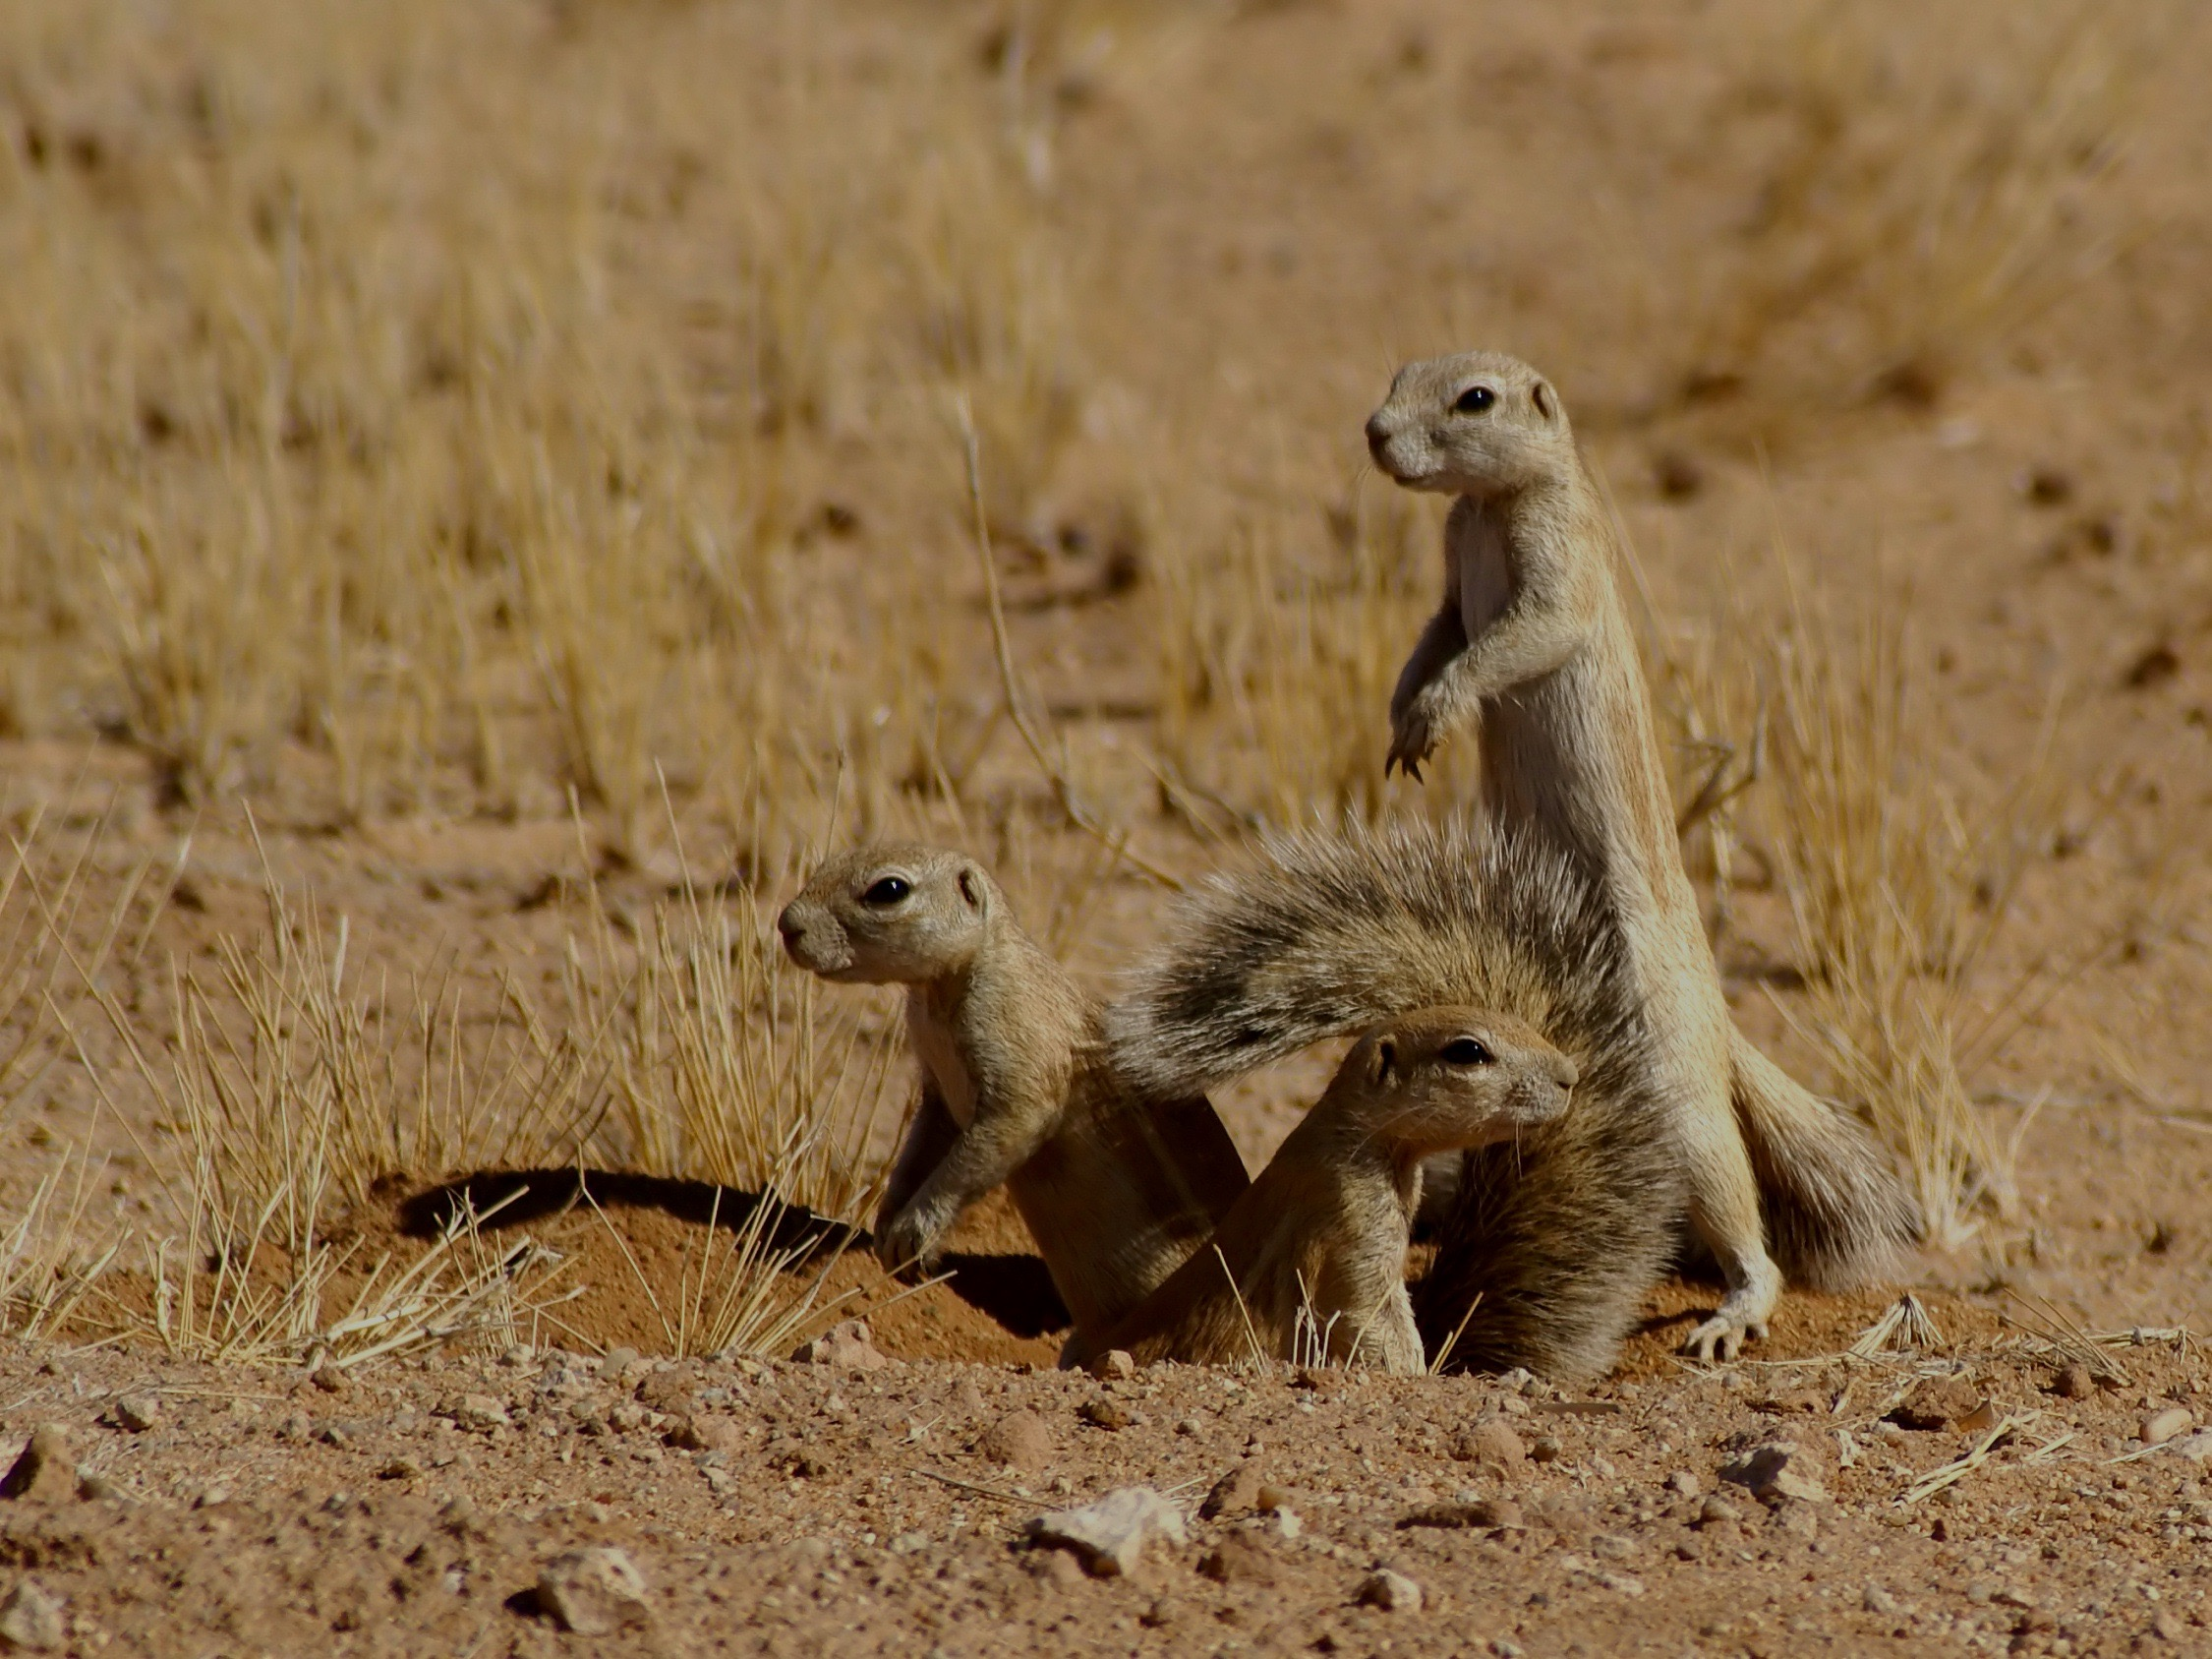
\includegraphics[width=\paperwidth,%
                   keepaspectratio=true]{images/Xerus_inauris_1}
\end{textblock*}

%% titre
\begin{textblock*}{\textwidth}(\TPHorizModule,6\TPVertModule)
  \textcolor{black!5}{\titlefmt}
\end{textblock*}

%% auteur
\begin{textblock*}{\textwidth}(\TPHorizModule,11.5\TPVertModule)
  \textcolor{black!5}{\authorfmt}
\end{textblock*}

\null\cleardoublepage

%%%
%%% Page frontispice
%%%

%% titre
\begin{textblock*}{\textwidth}(\TPHorizModule,6\TPVertModule)
  \titlefmt
\end{textblock*}

%% auteur
\begin{textblock*}{\textwidth}(\TPHorizModule,11.5\TPVertModule)
  \authorfmt
\end{textblock*}

%% affiliation
\begin{textblock*}{\textwidth}(\TPHorizModule,15.5\TPVertModule)
  \affiliation
\end{textblock*}

%% édition
\begin{textblock*}{\textwidth}(\TPHorizModule,58\TPVertModule)
  \edition
\end{textblock*}
\endgroup

%%% Local Variables:
%%% mode: latex
%%% TeX-master: "programmer-avec-r"
%%% TeX-engine: xetex
%%% End:

\null\cleardoublepage           % cf. section 2.2 textpos.pdf

%%% Copyright (C) 2018 Vincent Goulet
%%%
%%% Ce fichier fait partie du projet
%%% «Programmer avec R»
%%% https://gitlab.com/vigou3/programmer-avec-r
%%%
%%% Cette création est mise à disposition selon le contrat
%%% Attribution-Partage dans les mêmes conditions 4.0
%%% International de Creative Commons.
%%% https://creativecommons.org/licenses/by-sa/4.0/

\begingroup
\calccentering{\unitlength}
\begin{adjustwidth*}{\unitlength}{-\unitlength}
  \setlength{\parindent}{0pt}
  \setlength{\parskip}{\baselineskip}
  \small

  \raisebox{-2.5mm}{%
    
\includegraphics[height=7mm,keepaspectratio=true]{images/by-sa}} %
  \raisebox{-2.5mm}{%
    
\includegraphics[height=7mm,keepaspectratio=true]{images/by-nc-sa}} %
  {\theauthor}, {\year}

  {\textcopyright} {\year} par {\theauthor}. «\thetitle», à
  l'exception les sections
  \ref*{sec:git:getting_started}--\ref*{sec:git:branching}, est mis à
  disposition selon le contrat
  \href{https://creativecommons.org/licenses/by-sa/4.0/deed.fr}{%
    Attribution-Partage dans les mêmes conditions 4.0 International}
  de Creative Commons. En vertu de ce contrat, vous êtes libre de:
  \begin{itemize}
  \item \textbf{partager} --- reproduire, distribuer et communiquer
    l'œuvre;
  \item \textbf{remixer} --- adapter l'œuvre;
  \item utiliser cette œuvre à des fins commerciales.
  \end{itemize}
  Selon les conditions suivantes:

  \begin{tabularx}{\linewidth}{@{}lX@{}}
    \raisebox{-9mm}[0mm][13mm]{%
      
\includegraphics[height=11mm,keepaspectratio=true]{images/by}}
    & \textbf{Attribution} --- Vous devez créditer l'œuvre, intégrer
    un lien vers le contrat et indiquer si des modifications ont été
    effectuées à l'œuvre. Vous devez indiquer ces informations par
    tous les moyens possibles, mais vous ne pouvez suggérer que
    l'Offrant vous soutient ou soutient la façon dont vous avez utilisé
    son œuvre. \\
    \raisebox{-9mm}{
\includegraphics[height=11mm,keepaspectratio=true]{images/sa}}
    & \textbf{Partage dans les mêmes conditions} --- Dans le cas où vous
    modifiez, transformez ou créez à partir du matériel composant
    l'œuvre originale, vous devez diffuser l'œuvre modifiée dans
    les même conditions, c'est à dire avec le même contrat avec lequel
    l'œuvre originale a été diffusée.
  \end{tabularx}

  Les sections
  \ref*{sec:git:getting_started}--\ref*{sec:git:branching} sont
  dérivées de «Pro Git» de Scott Chacon et Ben Straub sous contrat
  \href{https://creativecommons.org/licenses/by-nc-sa/3.0/deed.fr}{%
    Attribution-Pas d’utilisation commerciale-Partage dans les mêmes
    conditions 3.0 non transposé} de Creative Commons. Ce contrat
  ajoute aux conditions ci-dessus:

  \begin{tabularx}{\linewidth}{@{}lX@{}}
    \raisebox{-9mm}[0mm][13mm]{%
      
\includegraphics[height=11mm,keepaspectratio=true]{images/nc}}
    & \textbf{Pas d’utilisation commerciale} --- Vous n'êtes pas
    autorisé à faire un usage commercial de cette œuvre, tout ou
    partie du matériel la composant.
  \end{tabularx}

  \textbf{Code source} \\
  \viewsource{\reposurl}

  \textbf{Couverture} \\
  Groupe d'écureuils de terre du Cap (\emph{Xerus inauris}) sortant de
  leur terrier près de Solitaire, dans le désert du Namib, en Namibie.

  Crédit photo: {\textcopyright} Hans Hillewaert,
  \href{https://creativecommons.org/licenses/by-sa/3.0/deed.fr}{CC BY-SA 3.0}, via
  \href{https://commons.wikimedia.org/w/index.php?curid=2429056}{Wikimedia Commons}.
\end{adjustwidth*}
\endgroup

%%% Local Variables:
%%% mode: latex
%%% TeX-engine: xetex
%%% TeX-master: "programmer-avec-r"
%%% coding: utf-8
%%% End:

\clearpage

\pagestyle{companion}

%%% Copyright (C) 2020 Vincent Goulet
%%%
%%% Ce fichier fait partie du projet
%%% «Programmer avec R»
%%% https://gitlab.com/vigou3/programmer-avec-r
%%%
%%% Cette création est mise à disposition sous licence
%%% Attribution-Partage dans les mêmes conditions 4.0
%%% International de Creative Commons.
%%% https://creativecommons.org/licenses/by-sa/4.0/

\chapter{Introduction}
\markboth{Introduction}{Introduction}

Cet ouvrage traite de programmation informatique --- ou de codage,
pour utiliser le terme de plus en plus courant. À l'aube d'une
révolution numérique et de l'industrie 4.0, la programmation devient
une compétence essentielle chez les étudiants comme chez les
travailleurs du vingt-et-unième siècle. De même, la place sans cesse
grandissante accordée à la science des données --- analyse prédictive,
apprentissage profond, intelligence artificielle --- dans la plupart
des disciplines scientifiques ne fait qu'accentuer l'importance de
disposer d'une solide formation en programmation.

Les principaux buts du présent ouvrage sont donc: d'abord de
développer une culture de l'informatique; ensuite d'acquérir la
capacité à résoudre des problèmes concrets à l'aide de l'algorithmique
et de la programmation; enfin de se familiariser avec les bonnes
pratiques reconnues en contexte de travail collaboratif, puisque la
programmation se pratique beaucoup plus souvent en groupe que seul.

Vous apprendrez à programmer en R, le langage au coeur de
l'environnement statistique du même nom et l'un des outils les plus
utilisés dans le monde pour l'analyse de données. Le système R connait
depuis plus d'une décennie une progression remarquable dans ses
fonctionnalités, dans la variété de ses domaines d'application ou,
plus simplement, dans le nombre de ses utilisateurs. La documentation
sur l'utilisation de R en sciences naturelles, en sciences sociales,
en finance, etc, ne manque pas. Cependant, peu d'ouvrages se
concentrent sur l'apprentissage de R en tant que langage de
programmation sous-jacent aux fonctionnalités statistiques. C'est la
niche que je tâche d'occuper avec «Programmer avec R».

L'analyse de données requiert souvent de manipuler ou de traiter du
texte. Par conséquent, l'ouvrage aborde également les expressions
régulières et divers utilitaires d'analyse et de contrôle de texte.

Enfin, vous trouverez en annexe de brèves introductions à
l'environnement de développement intégré RStudio et à l'éditeur de
texte pour programmeurs GNU~Emacs, de même que les solutions complètes
des exercices.

\section*{Formation concomitante}

Certaines parties de l'ouvrage tablent sur des connaissances de base
dans l'utilisation d'une ligne de commande Unix et d'un système de
gestion de versions. Ma formation concomitante «Ligne de commande et
gestion de versions avec Git» \citep{Goulet:laboratoire-cli-git:2020}
permet d'acquérir ces connaissances.

La ligne de commande est la plus ancienne des interfaces avec les
ordinateurs. Si les interfaces graphiques ont à plusieurs égards
grandement facilité l'interaction homme-machine, elles n'ont pas pour
autant fait disparaitre ou rendu obsolète la ligne de commande, tout
particulièrement dans la pratique de la programmation.

Outil essentiel en contexte de travail collaboratif, le système de
gestion de versions permet de régler les problèmes de suivi de la plus
récente version d'un fichier, de partage de fichiers entre les membres
d'une équipe et de mise en commun des contributions. Développé par
Linus Torvalds pour administrer le code source du noyau du système
d'exploitation Linux, \link{https://git-scm.com}{Git} est aujourd'hui
le système de gestion de versions le plus utilisé dans le monde.


\section*{Utilisation de l'ouvrage}

L'ouvrage vise d'abord à vous exposer à un maximum de code, puis à
vous faire pratiquer. C'est pourquoi plusieurs chapitres sont rédigés
de manière synthétique et qu'ils comportent peu d'exemples au fil du
texte.

En revanche, vous devrez lire et évaluer le code informatique se
trouvant dans les sections d'exemples à la fin de la plupart des
chapitres. Ce code et les commentaires qui l'accompagnent reviennent
sur l'essentiel des concepts du chapitre et les complémentent souvent.
Je considère l'exercice d'«étude active» consistant à évaluer du code
et à voir ses effets comme essentiel à l'apprentissage de la
programmation. Vous pouvez aussi inverser la proposition et étudier le
code informatique avant le texte du chapitre correspondant si ce mode
d'apprentissage vous convient mieux.

Le code des sections d'exemples est distribué avec le document sous
forme de fichiers de script. De plus, à chaque fichier \code{.R}
correspond un fichier \code{.Rout} contenant les résultats de son
évaluation non interactive.


\section*{Fonctionnalités interactives}

En consultation électronique, ce document se trouve enrichi de
plusieurs fonctionnalités interactives.
\begin{itemize}
\item Intraliens du texte vers une ligne précise d'une section de code
  informatique et, en sens inverse, du numéro de la ligne vers le
  point de la référence dans le texte. Ces intraliens sont marqués par
  la couleur \textcolor{link}{\rule{1.5em}{1.2ex}}.
\item Intraliens entre le numéro d'un exercice et sa solution, et vice
  versa. Ces intraliens sont aussi marqués par la couleur
  \textcolor{link}{\rule{1.5em}{1.2ex}}.
\item Intraliens entre les citations dans le texte et leur entrée dans
  la bibliographie. Ces intraliens sont marqués par la couleur
  \textcolor{citation}{\rule{1.5em}{1.2ex}}.
\item Hyperliens vers des ressources externes marqués par le symbole
  {\smaller\faExternalLink*} et la couleur
  \textcolor{url}{\rule{1.5em}{1.2ex}}.
\item Table des matières, liste des tableaux, liste des figures et
  liste des vidéos permettant d'accéder rapidement à des ressources du
  document.
\item Index comprenant, entre autres, les principaux mots clés du
  langage R et toutes leurs occurrences dans le texte ainsi que
  dans le code informatique.
\end{itemize}

\section*{Blocs signalétiques}

Le document est parsemé de divers types de blocs signalétiques
inspirés de
\link{https://asciidoctor.org/docs/user-manual/\#admonition}{AsciiDoc}
qui visent à attirer votre attention sur une notion.

\tipbox{Astuce! Ces blocs contiennent un truc, une astuce, ou tout
  autre type d'information utile.}
\vspace{-\baselineskip}

\warningbox{Avertissement! Ces blocs mettent l'accent sur une notion
  ou fournissent une information importante pour la suite.}
\vspace{-\baselineskip}

\cautionbox{Attention! Vous risquez de vous bruler ---
  métaphoriquement, s'entend --- si vous ne suivez pas les
  recommandations de ces blocs.}
\vspace{-\baselineskip}

\importantbox{Important! Ces blocs contiennent les remarques les plus
  importantes. Veillez à en tenir compte.}
\vspace{-\baselineskip}

\notebox{Ces blocs contiennent des remarques additionnelles sur
  la matière ou des informations amusantes, mais non essentielles.}
\vspace{-\baselineskip}

%% Utilisation de la commande \awesomebox pour illustrer les blocs de
%% vidéos pour éviter de créer une entrée dans la liste des vidéos.
\awesomebox{\aweboxrulewidth}{\faYoutube}{url}{Ces blocs
  contiennent des liens vers des vidéos dans ma %
  \link{https://www.youtube.com/user/VincentGouletIntroR/videos}{chaine
    YouTube}. Les vidéos sont répertoriées dans la liste des vidéos.}
\vspace{-\baselineskip}

\gotorbox{Ces blocs vous invitent à interrompre la lecture du texte
  pour passer à l'étude du code R des sections d'exemples.}
\vspace{-\baselineskip}

\osxbox{Remarques spécifiques à macOS.}
\vspace{-\baselineskip}

\windowsbox{Remarques spécifiques à Windows.}

\section*{Document libre}

Tout comme R et l'ensemble des outils présentés dans ce document, le
projet «Programmer avec R» s'inscrit dans le mouvement de
l'\link{https://www.gnu.org/philosophy/free-sw.html}{informatique
  libre}. Vous pouvez accéder à l'ensemble du code source en format
{\LaTeX} en suivant le lien dans la page de copyright. Vous trouverez
dans le fichier \code{README.md} toutes les informations utiles pour
composer le document.

Votre contribution à l'amélioration du document est également la
bienvenue; consultez le fichier \code{CONTRIBUTING.md} fourni avec ce
document et voyez votre nom ajouté au fichier \code{COLLABORATEURS}.

Bonne lecture!

%%% Local Variables:
%%% mode: latex
%%% TeX-engine: xetex
%%% TeX-master: "programmer-avec-r"
%%% coding: utf-8
%%% End:


\tableofcontents*
\cleartorecto
\listoftables*
\cleartorecto
\listoffigures*

%% Vignette tirée de xkcd.com
\cleartoverso
\thispagestyle{empty}
\begin{vplace}[0.45]
  \centering
  \begin{minipage}{0.9\linewidth}
    \setkeys{Gin}{width=\textwidth}
    \includegraphics{images/compiling.png} \\
    \footnotesize\sffamily%
    Tiré de \href{http://xkcd.com/303/}{XKCD.com}
  \end{minipage}
\end{vplace}

\mainmatter

%%% Copyright (C) 2018 Vincent Goulet
%%%
%%% Ce fichier fait partie du projet
%%% «Programmer avec R»
%%% https://gitlab.com/vigou3/programmer-avec-r
%%%
%%% Cette création est mise à disposition selon le contrat
%%% Attribution-Partage dans les mêmes conditions 4.0
%%% International de Creative Commons.
%%% https://creativecommons.org/licenses/by-sa/4.0/

\chapter{Éléments d'informatique pour programmeurs}
\label{chap:informatique}

\begin{objectifs}
\item Nommer et ordonner les grands jalons de l'histoire des langages
  de programmation.
\item Identifier les principaux paradigmes de programmation.
\item Distinguer les concepts de syntaxe et de sémantique d'un langage
  de programmation.
\item Distinguer les concepts de langage compilé et de langage
  interprété.
\item Comparer les forces et faiblesses de divers langages de
  programmation en fonction de divers critères.
\item Comprendre la structure du système de fichiers d'un ordinateur
  et identifier le chemin d'accès vers une ressource dans celui-ci.
\item Naviguer dans le système de fichiers d'un ordinateur et obtenir
  une liste des fichiers à partir d'une interface en ligne de
  commande.
\end{objectifs}

Vous savez programmer.

En effet, avec l'omniprésence des outils numériques dans notre vie
quotidienne, nous automatisons tous certaines tâches:
%%
demander une alarme pour le lendemain matin;
enregistrer une émission de télé qui sera diffusée dans trois jours;
planifier des virements entre comptes chez notre institution
  financière;
signaler du contenu ou interpeller quelqu'un sur les médias sociaux
  à l'aide des symboles \code{\#} et \code{@};
entrer un code de triche dans un jeu vidéo;
calculer la moyenne d'une colonne dans un tableur;
guider un robot vers la sortie d'un labyrinthe.
%%
Vous pouvez sans doute ajouter vos propres exemples à cette liste.

Dans chacun des exemples précités, l'utilisateur dicte à une machine
des tâches à effectuer en utilisant un langage qu'elle est à même de
comprendre. Que le langage soit excessivement simple ou qu'une
interface vous guide pas à pas dans la programmation n'y change
fondamentalement rien: vous programmez.

Cet ouvrage vise simplement à vous faire atteindre un niveau de
sophistication bien plus grand qui fera réellement de vous des
programmeuses et des programmeurs informatiques.

<description du chapitre>

\section{Qu'est-ce que programmer?}
\label{sec:informatique:programmer?}

Programmer est une activité scientifique consistant d'abord et avant
tout à \emph{résoudre des problèmes}. Plutôt que d'avoir recours aux
mathématiques ou à l'expérimentation, les programmeurs demandent à une
machine de résoudre le problème pour eux. Comme le souligne
\citet{Swinnen:python:2012} --- dont la lecture du chapitre~1 est
chaudement recommandée --- programmer est «une compétence de haut
niveau, qui implique des capacités et des connaissances diverses: être
capable de (re)formuler un problème de plusieurs manières différentes,
être capable d’imaginer des solutions innovantes et efficaces, être
capable d’exprimer ces solutions de manière claire et complète.»

La première difficulté réside toutefois dans le fait de «demander» à
une machine de résoudre un problème: il faut établir un mode de
communication pour que l'humain puisse dicter des instructions à une
machine qui, en définitive, ne comprend que deux instructions: vrai et
faux, ouvert ou fermé, 0 ou 1. C'est là le rôle du \emph{langage de
  programmation}.

Tout au long de leur histoire, les humains ont inventé une multitude
de langages pour échanger entre eux: langues parlées, écritures,
langues des signes, peinture, musique, etc. Certains langages
parviennent à mieux exprimer certaines réalités ou certains sentiments
que d'autres. Or, il en va de même des langages de programmation: non
seulement sont-ils nombreux, mais certains conviennent mieux à
certains types de tâches que d'autres. Vous serez à même d'apprécier
la diversité des langages de programmation à la lecture de la
\autoref{sec:informatique:historique} qui retrace les grands jalons de
leur histoire.

\subsection{Algorithme}
\label{sec:informatique:programmer:algorithme}

Vous avez probablement déjà trié une liste de mots à l'aide d'un
ordinateur. Pourtant, l'ordinateur n'a aucune connaissance du concept
d'ordre alphabétique. Et même s'il «connaissait» cet ordre, comment au
juste réalise-t-il l'opération de tri? Ce genre de questions relève de
l'une des pierres d'assise de l'informatique:
l'\index{algorithmique}algorithmique, la science qui étudie les
algorithmes et les structures de données.

Un \index{algorithme}\emph{algorithme} est une procédure de calcul
permettant de résoudre un problème bien spécifié. En cela,
l'algorithme explique comment, à partir d'entrants, obtenir l'extrant
solution du problème. Quand on y pense, ce n'est pas très différent
d'une recette culinaire où les entrants sont les ingrédients, la
procédure les étapes de la recette et les extrants, le mets.

L'algorithmique est une discipline riche en techniques ingénieuses et
en analyses mathématiques poussées. Connaitre ses principes de base et
les algorithmes classiques permet de mieux planifier ses méthodes de
résolution de problème. En effet, un bon algorithme permet de résoudre
en quelques secondes un problème qui pourrait autrement prendre des
années.

À titre d'exemple, supposons que vous devez calculer, pour un jeu de
données quelconque, l'écart moyen des données supérieures à $12$ par
rapport à cette valeur. Un premier algorithme de très haut niveau
permettant de résoudre ce problème irait comme suit.

\begin{Schunk}
  \begin{enumerate}
  \item Sélectionner les données supérieures à $12$.
  \item Soustraire $12$ de chaque valeur retenue à la première étape.
  \item Effectuer la moyenne des valeurs obtenues à la seconde étape.
  \end{enumerate}
\end{Schunk}

Apportons une toute petite modification à l'algorithme ci-dessus.

\begin{Schunk}
  \begin{enumerate}
  \item Sélectionner les données supérieures à $12$.
  \item Effectuer la moyenne des valeurs obtenues à la première étape.
  \item Soustraire $12$ de la valeur retenue à la seconde étape.
  \end{enumerate}
\end{Schunk}

Mathématiquement, les deux approches sont tout à fait équivalentes.
Cependant, avec la première approche, nous effectuons une soustraction
pour chaque valeur supérieure à $12$ que compte jeu de données. Avec
la seconde approche, nous n'effectuons qu'une seule soustraction. Si
le jeu de données compte un million d'entrées supérieures à $12$,
c'est un million de soustractions contre une seule. En temps de
calcul, cela ne représente qu'un écart de quelques centièmes de
secondes sur un ordinateur moderne, mais ces fractions de secondes
peuvent finir par faire une différence importante lorsque la taille
des jeux de données augmente ou lorsque l'opération se répète de
nombreuses fois.

Attardons-nous à un second exemple intéressant: l'élévation d'une
valeur $b$ à la puissance $n$. Un premier algorithme, écrit cette fois
en \index{pseudo-langage}\emph{pseudo-langage}, pourrait se lire
ainsi.

\begin{Schunk}
\begin{Verbatim}
Puissance(nombre réel b, entier n)
  Si n = 0, retourner 1.
    Retourner b * Puissance(b, n - 1).
Fin Puissance
\end{Verbatim}
\end{Schunk}

Cet algorithme est \index{algorithme|récursif}\emph{récursif}: la
procédure \code{Puissance} s'appelle elle-même à répétition jusqu'à
l'obtention du résultat désiré. Mathématiquement, l'algorithme revient
à calculer $b^n$ de la manière la plus simple et intuitive qui soit:
\begin{equation*}
  b^n = b (b (b \cdots (b))).
\end{equation*}
Cela peut convenir lorsque $n$ est petit, mais peut-on faire mieux
pour une «grande» valeur de $n$? Imaginez que vous ne disposez que
d'une calculatrice munie des opérations arithmétiques de base et du
carré, et que vous devez élever un nombre à la puissance, disons,
$21$. Comment feriez-vous pour réduire le nombre d'opérations à entrer
au clavier?

\notebox{Cet exemple est moins fantaisiste qu'il n'y parait. Jusqu'au
  milieu des années 1990, les étudiants en actuariat ne disposaient
  que de ce type de calculatrice pour les examens professionnels! Le
  modèle en question de Texas Instruments était affectueusement nommé
  «TI 0».}

Vous avez pensé à un «algorithme»? Votre idée consiste fort
probablement à diviser la puissance par deux autant de fois que
possible et à élever au carré par la suite. Dans notre exemple, cela
donne
\begin{align*}
  b^{21}
  &= b (b^{20}) \\
  & = b (b^{10})^2 \\
  &= b ((b^5)^2)^2 \\
  & = b ((b (b^4))^2)^2 \\
  &= b ((b (b^2)^2)^2)^2.
\end{align*}
Ce calcul se traduit en algorithme comme suit.

\begin{Schunk}
\begin{Verbatim}
Puissance(nombre réel b, entier n)
  Si n = 0, retourner 1.
    Si n est pair, retourner (Puissance(b, n/2))^2.
    Si n est impair, retourner b * Puissance(b, n - 1).
Fin Puissance
\end{Verbatim}
\end{Schunk}

Pour élever un nombre à la puissance $21$, le premier algorithme
requiert $20$ opérations et le second, seulement $6$. Le dénombrement du
nombre d'opérations requis par un algorithme est un aspect important
de leur analyse. Il se fait généralement en notation $O()$ qui
signifie «de l'ordre de». Dans le premier algorithme de calcul de
$b^n$, le nombre d'opérations est directement proportionnel à $n$,
donc on dit que l'algorithme est $O(n)$. Dans le second algorithme où
la puissance est divisée par deux à répétition, le nombre d'opérations
est proportionnel au logarithme (en base deux) de $n$, d'où un
algorithme $O(log n)$.

\citet{Kernighan:practice:1999} font remarquer fort à propos que «si
tous les programmes reposent sur des algorithmes, très peu de
programmes exigent d'en concevoir de nouveaux». Autrement dit, aussi
complexe soit-il, un programme repose souvent sur quelques algorithmes
fondamentaux bien connus et bien établis. À ce titre, les algorithmes
de tri et de recherche jouent un rôle particulièrement important: on
estime que 25~\% du temps de calcul des ordinateurs est consacré au
tri et à la recherche! Ce n'est pour rien que Donald Knuth consacre un
volume entier de son œuvre monumentale \emph{The Art of Computer
  Programming} à ce seul sujet \citep{Knuth:ACP:vol1:1997}.


\subsection{Sémantique et syntaxe}
\label{sec:informatique:programmer:semantique}

Il y a plusieurs parallèles à dresser entre les langages de
programmation et les langues parlées ou écrites: leur apprentissage
requiert de la pratique; on en connait jamais un trop grand nombre; le
premier est plus difficile à apprendre que les suivants.
L'informatique a également emprunté à la linguistique les notions de
\index{sémantique}sémantique et de \index{syntaxe}syntaxe.

La sémantique est l'étude de ce que signifie un message ou un
programme informatique, c'est-à-dire de ce qu'il transmet ou exécute.
La syntaxe, quant à elle, étudie la structure du message ou du
programme. En simplifiant, disons que, pour une langue donnée, un
dictionnaire permet de connaitre la sémantique, alors qu'une grammaire
décrit la syntaxe \citep{Hebenstreit:semantique}.

Par exemple, exprimons le message «J'ai soif» en anglais. Dire
«\emph{I am hungry}» relèverait d'une erreur de sémantique, puisque la
signification du message s'en trouve changée. En revanche, avec
«\emph{I have thirsty}», le bon message se rendra, mais peut-être pas
sans que l'erreur de syntaxe n'ait d'abord suscité une hésitation chez
l'interlocuteur\footnote{%
  La formule correcte est «I am thirsty», soit littéralement «Je suis
  soif», en français.}.

Comme pour une langue, la maitrise d'un langage de programmation exige
de respecter à la fois les règles de sémantique et les règles de
syntaxe du langage. Le second volet est relativement facile: si le
programme compile ou s'exécute, c'est généralement que la syntaxe est
respectée. Le respect de la sémantique, ou de la manière propre d'un
langage d'exprimer des idées, demande plus d'efforts et de pratique.


\section{Bref historique des langages de programmation}
\label{sec:informatique:historique}

Ada Lovelace (1815--1852) est généralement reconnue comme la première
autrice d'un algorithme et de ce que l'on appelle aujourd'hui un
programme informatique. C'est en son honneur qu'a été nommé le langage
Ada conçu en réponse à un cahier de charges du département de la
Défense des États-Unis au début des années 1980.

Franchissons d'un bond les premiers jours de l'informatique et de la
programmation pour arriver aux ordinateurs électriques modernes, dans
les années 1940. On programme alors généralement ceux-ci en
\index{assembleur}assembleur, un langage de très bas niveau facilement
interprétable par la machine, mais difficile à lire par des humains,
comme l'extrait de programme de la
\autoref{fig:informatique:assembleur} le démontre bien.

\begin{figure}
  \centering
  \includegraphics[trim=0 475 0 0, clip=true]{images/Motorola_6800_Assembly_Language.png}
  \caption[Programme en assembleur pour un microprocesseur 8~bits
  Motorola 6800.]{Extrait d'un programme en assembleur pour un
    microprocesseur 8~bits Motorola 6800. {\small Source:
      \link{https://commons.wikimedia.org/wiki/File\%3AMotorola_6800_Assembly_Language.png}{Wikimedia
        Commons}}}
  \label{fig:informatique:assembleur}
\end{figure}

Les premiers langages créés pour transmettre des instructions à un
ordinateur apparaissent dans les années 1950. Ils sont à l'origine
intimement liés à l'architecture d'un ordinateur: à chaque type
d'ordinateur son langage de programmation. Certaines contraintes ---
ou exigences --- des langages de l'époque proviennent aussi du support
physique alors utilisé pour stocker les programmes: les cartes
perforées.

\subsection{Fortran}
\label{sec:informatique:historique:fortran}

En 1954, l'ingénieur de IBM John Backus publie les spécifications du
langage \index{Fortran}FORTRAN (\emph{FORmula TRANslating System}). Le
premier compilateur voit le jour deux ans plus tard. Fortran (avec des
minuscules à partir de 1977) deviendra rapidement le langage standard
dans le calcul scientifique.

Plus d'un demi-siècle plus tard, l'empreinte de Fortran demeure
importante, notamment grâce aux bibliothèques d'algèbre linéaire
BLAS\footnote{%
  \emph{Basic Linear Algebra Subprograms};
  \link{http://www.netlib.org/blas}{}.} %
et LAPACK\footnote{%
  \emph{Linear Algebra PACKage};
  \link{http://www.netlib.org/lapack}{}.} %
auxquelles ont recours la plupart des progiciels scientifiques, dont
R. Le langage est toujours utilisé en calcul haute performance et pour
mesurer le rendement des superordinateurs.

\notebox{Dans le très recommandable film «Les figures de l'ombre»
  (\emph{Hidden Figures}, 2016), une des héroïnes entreprend de
  s'attaquer à la programmation des nouveaux ordinateurs de la NASA.
  On peut alors voir qu'elle apprend le Fortran.}

\subsection{Lisp}
\label{sec:informatique:historique:lisp}

Le deuxième langage le plus ancien toujours largement diffusé est
\index{Lisp}Lisp (\emph{LISt Processing}). Créé par John McCarthy en
1958 en tant que modèle pratique pour représenter des programmes, le
Lisp est devenu le langage de choix pour la recherche et les
applications en intelligence artificielle. Le terme Lisp désigne
aujourd'hui une famille de langages comprenant de nombreux dialectes,
dont Common Lisp, Scheme et Emacs Lisp.

Le Lisp se distingue en outre par une syntaxe simple en
\index{notation!préfixée}notation préfixée (voir encadré), le support
pour la programmation fonctionnelle
(\autoref{sec:informatique:paradigmes}) et la faculté de manipuler le
code source en tant que structure de données. Autre trait distinctif:
la syntaxe du Lisp fait un usage immodéré des parenthèses.

Le Lisp est entouré d'une aura de beauté et d'élégance dont peu
d'autres langages peuvent se targuer. Citons Eric Raymond dans
\link{http://www.catb.org/esr/faqs/hacker-howto.html}{\emph{How to
    Become a Hacker}}:
\begin{quote}
  Il faut apprendre le Lisp pour l'extraordinaire expérience d'éveil
  [\emph{enlightenment experience}] que procure le fait de finalement
  le comprendre; cette expérience fera de vous un meilleur programmeur
  pour toujours, même si vous n'avez plus vraiment à utiliser le Lisp.
\end{quote}

Pour illustrer encore davantage la place toute particulière qu'occupe
le Lisp en programmation, mentionnons également l'aphorisme selon
lequel «ceux qui ne connaissent pas le Lisp sont condamnés à le
réinventer», d'une certaine façon la version courte de la célèbre
\link{https://en.wikipedia.org/wiki/Greenspun\%27s_tenth_rule}{\emph{Greenspun's
    tenth rule of programming}}: %
\begin{quote}
  Tout programme suffisamment complexe en C ou en Fortran comporte une
  mise en œuvre mal spécifiée, pleine de bogues et lente de la moitié
  de Common Lisp.
\end{quote}
(Fait amusant à noter: il n'y a pas d'autres lois que la dixième, de
l'\link{http://philip.greenspun.com/bboard/q-and-a-fetch-msg?msg_id=000tgU}{aveu
  même de l'auteur}.)

\begin{figure}[t]
  \label{fig:informatique:notations}
  \setlength{\FrameRule}{1pt}
  \lstset{backgroundcolor=\color{codebg},
    frame=lr, rulecolor=\color{codebg},
    xleftmargin=3.4pt, xrightmargin=3.4pt}
  \begin{emphbox}{\mdseries Notations infixée, préfixée et suffixée}
    Les notations \index{notation!infixée}infixée (\emph{infix}),
    \index{notation!préfixée}préfixée (\emph{prefix}) et
    \index{notation!suffixée}suffixée (\emph{postfix}) sont trois
    manières différentes, mais équivalentes, d'écrire des expressions
    en mathématiques ou en programmation.

    Par exemple, l'opération d'addition de deux opérandes $x$ et $y$
    s'écrit en notation infixée
\begin{lstlisting}
x + y
\end{lstlisting}
    En notation préfixée, aussi appelée notation polonaise,
    l'opérateur est placé avant les opérandes:
\begin{lstlisting}
+ x y
\end{lstlisting}
    On l'aura compris, en notation suffixée, ou notation polonaise
    inversée, l'opérateur apparait après les opérandes:
\begin{lstlisting}
x y +
\end{lstlisting}
    Nous sommes davantage habitués à lire la notation infixée, quoique
    la notation préfixée nous soit familière pour les opérateurs à un
    seul opérande (comme la négation) ou pour les appels de fonctions.
    La notation suffixée n'a jamais recours aux parenthèses.

    La compagnie HP commercialise de très prisées calculatrices
    scientifiques utilisant la notation suffixée (libellées RPN pour
    \emph{Reverse Polish Notation}) depuis 1972.
  \end{emphbox}
\end{figure}

\subsection{COBOL}
\label{sec:informatique:historique:cobol}

Le troisième langage développé dans les années 1950 et toujours en
usage de nos jours est \index{COBOL}COBOL (\emph{COmmon Business
  Oriented Language}). Ce langage spécialisé dans les applications de
gestion a été créé en 1959 par un comité formé pour proposer un
langage commun pour l'administration américaine.

Le COBOL reste très utilisé dans de grandes entreprises, notamment
dans les institutions financières. La légende urbaine veut d'ailleurs
que les programmeurs COBOL soient comparativement très bien rémunérés
aujourd'hui sous l'effet combiné de leur rareté et de l'importance
opérationnelle des applications qu'ils doivent maintenir.

\subsection{Algol}
\label{sec:informatique:historique:algol}

Dès la fin de la décennie 1950, un comité de scientifiques se réunit à
Zurich pour concevoir ce que l'on voudrait voir devenir le langage de
programmation standard. De ces rencontres naitra \index{Algol}Algol
(\emph{ALGorithmic Oriented Language}) en 1958. Comme la plupart des
tentatives de définition d'un standard, c'est un échec: le langage est
populaire dans les milieux académiques, mais restera peu utilisé dans
les applications commerciales.

Cela dit, on doit à Algol plusieurs innovations importantes, de telle
sorte qu'un grand nombre des langages qui verront le jour par la suite
seront considérés comme ses descendants; le poster
\link{http://www.oreilly.com/go/languageposter}{\emph{History of
    Programming Languages}} de O'Reilly Media illustre ceci à
merveille. \citet{Hoare:1973} a d'ailleurs cette jolie formule:
\begin{quote}
  Voici un langage très en avance sur son temps, il n'a pas seulement
  été une amélioration de ses prédécesseurs mais aussi une
  amélioration de presque tous ses successeurs.
\end{quote}

\begin{figure}[t]
  \centering
  \begin{minipage}{0.9\linewidth}
    \setkeys{Gin}{width=\textwidth}
    \includegraphics{images/standards} \\
    \footnotesize\sffamily%
    Tiré de \href{http://xkcd.com/927/}{XKCD.com}
  \end{minipage}
\end{figure}

\subsection{APL}
\label{sec:informatique:historique:apl}

Notre historique ne serait pas complet sans un mot sur \index{APL}APL
(\emph{A Programming Language}, qui l'aurait cru). Même s'il n'a
jamais connu une diffusion importante, ce langage conçu par Kenneth
Iverson autour de 1962 n'en a pas moins eu une influence considérable
sur la manière de penser et de représenter les opérations
mathématiques sur les tableaux à plusieurs dimensions.

Doté d'une large gamme de symboles pour représenter des opérations et
d'une syntaxe tout à fait particulière --- les expressions sont
exécutées de droite à gauche! --- l'APL est remarquablement concis et
puissant; voir la \autoref{fig:informatique:apl} pour un aperçu. Le
revers de la médaille et ce qui a assurément nui à son adoption
à large échelle, c'est la difficulté que l'on éprouve à relire le
code. Assez pour que d'aucuns qualifient l'APL de «langage à écriture
seulement».

APL a pendant longtemps été un langage très prisé par les actuaires,
aussi subsiste-t-il du code dans certaines compagnies d'assurance. Le
modèle de traitement des vecteurs, matrices et tableaux de l'APL a
servi d'inspiration pour la conception du langage S --- nous y
reviendrons au \autoref{chap:presentation}.

Le langage continue sa vie aujourd'hui principalement sous forme de son
successeur, \index{J}J.

\begin{figure}
  \centering
  \scalebox{0.4}{\includegraphics{images/APL_intro}}
  \caption[Opérations simples en APL.]{Opérations simples en APL. De
    haut en bas: génération des nombres de $1$ à $5$ et stockage dans
    la variable \code{x}; affichage du contenu de \code{x}; somme des
    éléments de \code{x}; moyenne des éléments de \code{x}. {\small Source:
    François-Dominique,
    \link{https://commons.wikimedia.org/w/index.php?curid=43207460}{Wikimedia
      Commons}, CC BY-SA 4.0}}
  \label{fig:informatique:apl}
\end{figure}

\subsection{C}
\label{sec:informatique:historique:c}

Le langage \index{C}C a été inventé en 1972 chez Bell Labs par Ken
Thompson et Dennis Ritchie afin de réécrire le système d'exploitation
UNIX (\autoref{sec:informatique:os:unix}). Il demeure beaucoup utilisé
pour la programmation système: le noyau de systèmes d'exploitation
comme Windows et Linux sont développés en grande partie en C.

Le C est un langage de programmation généraliste considéré, selon les
standards actuels, comme de bas niveau. Pour illustrer, l'utilisateur
doit programmer des traitements comme la libération de la mémoire, la
vérification de la validité des indices sur les tableaux, l'ouverture
et la fermeture des fichiers, etc.

Le langage demeure l'un des plus utilisés dans le monde et son
influence est considérable. De nombreux langages plus modernes comme
\index{C++@\Cpp}\Cpp, \index{C#@C\#}C\# et \index{Java}Java reprennent des
aspects de C. Le C est également beaucoup utilisé pour le calcul
numérique intensif, où il s'est en quelque sorte substitué à Fortran.
La plupart des progiciels scientifiques --- dont R, encore une fois
--- offrent la possibilité d'appeler du code C lorsque la rapidité de
calcul devient un enjeu. Le gain en temps d'exécution doit toutefois
être suffisamment grand pour compenser le temps de développement plus
long qu'exige le C par rapport à des langages de plus haut niveau.

\notebox{Dans l'ouvrage classique de \cite{KandR:1978}, le premier
  exemple d'un programme C affiche le message «\emph{hello, world}» à
  l'écran. Ça deviendra ensuite une tradition de démontrer le
  fonctionnement ou la syntaxe d'un langage avec cet exemple.}

\subsection{Autres jalons}
\label{sec:informatique:historique:autres}

Nous nous sommes attardés jusqu'ici à des langages de programmation
vieux de plus de 40 ans à cause de leur importance historique et parce
qu'ils sont toujours utilisés couramment. De nombreux autres langages
ont vu le jour depuis, si bien qu'ils se comptent aujourd'hui par
milliers. En voici quelques autres ayant occupé une place
prépondérante dans l'histoire.

\begin{itemize}
\item Comme son nom l'indique, \index{C++@\Cpp}\textbf{\Cpp} (Bjarne
  Stroustrup, 1980) est un dérivé du C qui lui ajoute, en autres
  choses, la programmation orientée objet. Certains considèrent que
  {\Cpp} devrait être le point d'entrée de toute personne voulant
  débuter à programmer avec des langages de la famille du C. Le code C
  est compatible avec le \Cpp.
\item Principal représentant de l'ère Internet des années 1990,
  \index{Java}\textbf{Java} (James Gosling, 1995) a été conçu pour
  que le code écrit dans ce langage puisse s'exécuter sur n'importe
  quelle plateforme informatique sans nécessiter une nouvelle
  compilation. Il est donc très populaire dans les applications web ou
  embarquées. Sa syntaxe est fortement inspirée du \Cpp.
\item \index{Visual Basic}\textbf{Visual Basic} (Microsoft, 1991) permet de développer des
  applications de manière interactive en disposant des composantes sur
  un canevas. Le langage est aujourd'hui discontinué, mais son dérivé
  \textbf{Visual Basic for Applications} (\index{VBA}VBA) demeure beaucoup
  utilisé dans les applications de la suite bureautique Office.
\item \index{Python}\textbf{Python} (Guido van Rossum, 1991) est un
  langage de haut niveau, orienté objet, multiplateforme et sous
  licence libre. C'est un des langages les plus utilisés aujourd'hui
  pour le calcul scientifique et l'analyse de données massives.
\end{itemize}

Certains langages de programmation ont une vocation généraliste,
certains visent des niches particulières, alors que d'autres cherchent
surtout à faire progresser l'état des connaissances dans la théorie
des langages. Quoi qu'il en soit, un langage de programmation demeure
un outil et, en informatique comme dans d'autres domaines, il convient
de choisir le meilleur outil pour accomplir une tâche donnée.

J'invite les lecteurs intéressés à en savoir davantage sur
l'histoire des langages de programmation en général, ou sur l'un ou
l'autre des langages mentionnés ci-dessus en particulier, à débuter
par les très complètes entrées de Wikipedia en
\link{https://fr.wikipedia.org/wiki/Histoire_des_langages_de_programmation}{français}
et en
\link{https://en.wikipedia.org/wiki/History_of_programming_languages}{anglais}.
\citet[chapitre~2]{Oualline:C:1997} propose également une excellente
introduction à la notion de programmation ainsi qu'une brève, mais
instructive, histoire du langage C.


\section{Langages compilés et interprétés}
\label{sec:informatique:compile_vs_interprete}

Tous les langages de programmation\footnote{%
  À l'exception du langage machine, mais rares sont les personnes qui
  souhaitent ne programmer qu'avec des $0$ et des $1$.} %
requièrent un traitement afin que les programmes écrits avec ceux-ci
puissent être exploités par un ordinateur. Il existe deux grandes
façons d'effectuer ce traitement: par compilation et par
interprétation.

Un \index{compilateur}compilateur est un programme informatique qui
transforme en langage machine le code source rédigé dans un langage
donné. On dit alors de ce langage qu'il est \index{compilé
  (langage)}\emph{compilé}. Le compilateur produit un fichier
informatique que l'ordinateur peut ensuite exécuter directement. Sur
la plateforme Windows, on reconnait notamment ces fichiers par leurs
extensions \code{.exe} ou \code{.dll}. Les noyaux d'à peu près toutes
les applications sur nos ordinateurs sont des fichiers compilés.

Un \index{interpréteur}interpréteur, quant à lui, est un programme qui
analyse, traduit et exécute le code source d'un programme
informatique, et ce, à chaque fois que le programme doit être exécuté.
Un langage qui nécessite l'intermédiaire d'un interpréteur est dit
\emph{interprété}. Un programme écrit dans un \index{interprété
  (langage)}langage interprété ne peut être distribué sans son
interpréteur.

Le traitement additionnel entre le code source et le langage machine
fait généralement en sorte que les langages interprétés sont plus
lents que les langages compilés à l'exécution. En revanche, une foule
de détails de mise en œuvre sont pris en charge par l'interpréteur, ce
qui réduit le temps de développement.


\section{Paradigmes de programmation}
\label{sec:informatique:paradigmes}

Un programme informatique est toujours écrit pour résoudre un problème
donné. Or, comme pour tout problème dans la vie, la solution à
celui-ci peut être formulée de différentes manières. Le style
fondamental avec lequel on exprime la solution est appelé le
paradigme de programmation.

Il existe plusieurs paradigmes de programmation. Nous nous
contenterons ici de se pencher sur seulement quatre.

\begin{description}
\item[Impératif] \index{paradigme!impératif} On indique à l'ordinateur
  les opérations à exécuter et l'ordre dans lequel les exécuter. C'est
  le paradigme le plus intuitif.
\item[Déclaratif] \index{paradigme!déclaratif} On indique cette fois à
  l'ordinateur ce que l'on souhaite obtenir comme résultat, mais sans
  préciser comment y parvenir. Il est laissé à la mise en œuvre du
  langage de déterminer la meilleure méthode de résolution du
  problème.

  Par exemple, pour extraire d'une base de données \code{etudiants} le
  prénom de toutes les personnes de plus de 25~ans, on écrira dans un
  langage déclaratif comme le SQL:
\begin{Schunk}
\begin{Verbatim}
SELECT prenom FROM etudiants WHERE age > 25
\end{Verbatim}
\end{Schunk}
  Nulle part n'est-il précisé comment le programme devrait procéder à
  l'extraction.
\item[Fonctionnel] \index{paradigme!fonctionnel} Un programme est une
  suite d'appels de fonctions, comme en mathématiques. L'exécution
  d'une fonction n'a pas d'impact sur les autres fonctions\footnote{%
    Autrement on dit qu'une fonction a un effet de bord (\emph{side
      effect}.} %
  Les opérations complexes sont réalisées en combinant les fonctions,
  de manière analogue à la composition de fonctions $g \circ f$.
\item[Orienté objet] \index{paradigme!orienté objet} Un programme est
  conçu comme un ensemble de blocs logiciels (les objets) qui
  interagissent entre eux. Une \emph{méthode} applique un traitement
  différent à un objet selon sa \emph{classe}. Ce paradigme est
  particulièrement utilisé dans les grands et complexes projets
  informatiques.
\end{description}

La plupart des langages d'usage courant combinent d'office, ou du
moins permettent de combiner, plusieurs paradigmes. Par exemple, le
langage {\Cpp} est à la fois un langage impératif et orienté objet.



\section{Systèmes d'exploitation}
\label{sec:informatique:os}

Le \index{système d'exploitation}système d'exploitation
(\emph{operating system}, OS) est un ensemble de programmes qui gère
les ressources matérielles et logicielles d'un ordinateur. Premier
programme exécuté par l'ordinateur lors de la mise en marche, le
système d'exploitation reçoit les demandes de ressources des
applications --- espace mémoire, unité de calcul, disque dur,
communication avec les périphériques, utilisation du réseau --- et les
alloue en fonction de l'état du système et des demandes concurrentes
des autres applications. Tous les logiciels applicatifs requièrent un
système d'exploitation pour fonctionner.

Il existe une grande variété de systèmes d'exploitation. Les plus
connus aujourd'hui sont, pour les ordinateurs personnels et les
serveurs, Windows de Microsoft, macOS de Apple et Linux, un logiciel
libre créé et toujours administré par Linus Torvalds. Pour les
appareils mobiles, deux systèmes d'exploitation se partagent
l'essentiel du marché: iOS et Android. Le premier est dérivé de macOS
et le second, de Linux.

Les systèmes macOS et Linux appartiennent à la famille des systèmes
Unix. Cela ne laisse donc en fait que deux grandes classes de systèmes
d'exploitation couramment utilisés: Windows et Unix.

\subsection{Windows}
\label{sec:informatique:os:windows}

Le système d'exploitation \index{Windows}Windows de Microsoft équipe
près de 90~\% des ordinateurs personnels dans le monde. Dans les
circonstances, rares sont les personnes qui n'ont jamais utilisé le
système, ne serait-ce qu'à petites doses.

À l'origine, en 1985, Windows n'était qu'une interface graphique
superposée au véritable système d'exploitation des ordinateurs de type
«compatibles IBM PC», le DOS. Les versions grand public depuis
Windows~2000 sont plutôt basées sur le noyau de Windows~NT, un système
conçu à partir de zéro et lancé au milieu des années 1990 en tant que
système pour les entreprises.

Le plus grand avantage de Windows est son ubiquité. À peu près toutes
les applications, sauf peut-être celles s'adressant à un segment de
marché très précis, sont disponibles sous Windows, en code natif, via
un port depuis Unix, ou encore par l'intermédiaire d'une couche
logicielle d'émulation comme Cygwin ou \index{MinGW}MinGW.

Un système d'exploitation multiutilisateur prend pour acquis que
plusieurs utilisateurs se partageront les ressources de l'ordinateur,
simultanément lorsqu'il s'agit d'un serveur, ou les uns après les
autres dans le cas d'un ordinateur personnel. Dans un tel système, on
établit des règles strictes d'accès aux ressources du système (seul
l'administrateur peut installer ou supprimer des applications) et
d'accès aux ressources des autres utilisateurs (Marianne n'a pas
accès aux fichiers d'Alexandre et vice-versa).

Les versions de Windows multiutilisateurs sont apparues relativement
tard sur le marché grand public, et ce, sans que le paradigme ne soit
imposé aux utilisateurs. Résultat: la plupart des utilisateurs de
Windows s'octroient à la ronde les droits d'administrateur et, pire,
plusieurs applications nécessitent toujours un accès total au système.
C'est par ces failles que se propagent virus et autres logiciels
malveillants sur la plateforme.

Les systèmes Windows sont livrés avec une trousse de développement
très restreinte. Les programmeurs doivent donc installer les outils
nécessaires, souvent sous forme de suites logicielles monolithiques,
ce qui entraine dédoublements et, parfois, conflits.

\subsection{Unix}
\label{sec:informatique:os:unix}

Le terme \index{Unix}\emph{Unix} --- ou UNIX qui, en majuscules, est
une marque déposée de \link{http://www.opengroup.org/unix}{Open Group}
--- recoupe une famille de systèmes d'exploitation dérivant tous du
premier système Unix développé chez Bell Labs dans les années 1970 par
Kenneth Thompson, Dennis Ritchie et plusieurs autres.

Les systèmes Unix partagent un certain nombre de caractéristiques
communes. D'abord, ils sont intrinsèquement multitâches et
multiutilisateurs. Ensuite, la
\Index{Unix!philosophie}\link{https://fr.wikipedia.org/wiki/Philosophie_d\%27Unix}{philosophie
  Unix} commande la modularité: le système d'exploitation fournit aux
utilisateurs (via un interpréteur de commandes, ou \emph{shell}) et
aux applications une multitude de petits outils très spécialisés qui
ne réalisent à peu près qu'une seule tâche. Le système rend ensuite
simple, via un mécanisme dit de transfert de données («tuyau»,
\emph{pipe}) de les combiner pour effectuer des opérations plus
complexes.

Par exemple, pour extraire le mot \emph{tuyau} du code source
contenant le précédent paragraphe, nous pourrions utiliser l'outil
\code{grep} pour extraire la ligne où se trouve le mot, puis l'outil
\code{cut} pour isoler le mot qui nous intéresse et, enfin, l'outil
\code{tr} pour supprimer la parenthèse ouvrante, les guillemets et la
virgule autour du mot.\footnote{%
  Dans la mesure où le mot que l'on recherche est le quatrième de la
  ligne dans le fichier source \code{informatique.tex}, la commande
  résultante est: \code{grep "«tuyau»" informatique.tex | cut -d " "
    -f 4 | tr -d \bs(«»,}\,. Le caractère \code{|} est l'opérateur de
  transfert de données.}

À l'exception notable des Mac, \index{Unix}Unix demeure assez peu répandu sur les
ordinateurs personnels. En revanche le système d'exploitation, en
particulier sa variante libre Linux, équipe l'immense majorité des
stations de travail, serveurs et supercalculateurs. De plus, bon
nombre d'applications scientifiques et de langages de programmation
sont d'abord développés sur des systèmes Unix. Pour ces
raisons, j'estime utile pour des programmeurs de connaitre les
quelques «Unix-ismes» ci-dessous.

\begin{itemize}
\item La barre oblique (\code{/}) est utilisée pour séparer les
  dossiers dans les chemins d'accès aux fichiers.
\item Tout utilisateur dispose d'un espace disque réservé identifié
  comme le \index{répertoire personnel}\emph{répertoire personnel} ou
  le \index{dossier de départ|see{répertoire personnel}}\emph{dossier
    de départ} (\emph{home directory}). Ce répertoire est situé dans
  \code{/Users} sous macOS et habituellement dans \code{/home} sous
  Linux.
\item À la ligne de commande et dans la configuration de plusieurs
  applications, le caractère \,\verb=~=\, représente le répertoire
  personnel.
\item Toujours à la ligne de commande, il est possible d'appuyer sur
  \code{TAB} pour compléter les noms de fichiers, de répertoires ou de
  commandes.
\item Plusieurs applications permettent de stocker des options de
  configuration sous forme de texte brut dans des fichiers dont le nom
  débute généralement par un point «\verb=.=»\,.
\end{itemize}
La section suivante fournit des détails additionnels sur le système de
fichiers de Unix.


\section{Systèmes de fichiers}
\label{sec:informatique:fs}

Le \index{système de fichiers}système de fichiers d'un ordinateur
contrôle l'inscription, l'organisation et la récupération des données
sur une unité de stockage, souvent un disque dur.

Nous n'entrerons pas dans les détails techniques des systèmes de
fichiers. Seulement, les programmeurs doivent être familiers avec
quelques grands principes de l'organisation des données dans un
ordinateur.

Les fichiers sont regroupés dans des répertoires. Ceux-ci contiennent
eux-mêmes des fichiers ou des sous-répertoires. Ce schéma se répète
sans limite pratique. Il en résulte une classification sous forme
d'arbre dont la \emph{racine} est le répertoire contenant
l'intégralité des fichiers. La \autoref{fig:informatique:fs} présente
des extraits des arbres de fichiers usuels de Windows et de macOS.

\begin{figure}
  \begin{minipage}[t]{0.45\linewidth}
    \dirtree{%
      .1 \code{C:\bs}.
      .2 \code{Program Files\bs}.
      .3 \code{Internet Explorer\bs}.
      .3 \code{Windows NT\bs}.
      .2 \code{Users\bs}.
      .3 \code{Alexandre\bs}.
      .4 \code{Desktop\bs}.
      .4 \code{Documents\bs}.
      .5 \code{synthese-1.doc}.
      .2 \code{Windows\bs}.
      .3 \code{explorer.exe}.
      .3 \code{System32\bs}.
      .4 \code{wininit.exe}.
    }
  \end{minipage}
  \hfill
  \begin{minipage}[t]{0.45\linewidth}
    \dirtree{%
      .1 \code{/}.
      .2 \code{/Applications}.
      .3 \code{/Mail.app}.
      .3 \code{/Preview.app}.
      .2 \code{/Users}.
      .3 \code{/Marianne}.
      .4 \code{/Desktop}.
      .5 \code{freestyle.txt}.
      .4 \code{/Documents}.
      .5 \code{/Cours}.
      .2 \code{/System}.
      .2 \code{/bin}.
      .3 \code{bash}.
      .2 \code{/usr}.
      .3 \code{/bin}.
      .4 \code{grep}.
    }
  \end{minipage}
  \caption[Extraits de la hiérarchie des systèmes de fichiers]{%
    Extraits des arbres de fichiers de Windows~7 (à gauche) et de
    macOS (à droite)}
  \label{fig:informatique:fs}
\end{figure}

\subsection{Particularités du système de fichiers de Windows}
\label{sec:informatique:fs:windows}

Sous Windows, chaque lecteur physique ou lecteur réseau dispose de son
propre arbre de fichiers. La racine est identifiée par une lettre. Le
premier disque dur est \code{C}\footnote{%
  La nomenclature des lecteurs date d'une époque où les ordinateurs
  personnels n'étaient pas tous équipés d'un disque dur, mais plutôt
  d'un ou deux lecteurs de disquettes. Ceux-ci étaient identifiés par
  les lettres \code{A} et \code{B}.}. %
Si le système comporte plus d'un disque, l'utilisateur doit savoir sur
quel disque retrouver ou enregistrer ses données.

Le système de fichiers de Windows est insensible à la casse,
c'est-à-dire qu'il ne fait aucune distinction entre \code{Program
  Files}, \code{program files} et \code{PROGRAM FILES}. Dans les
chemins d'accès (voir ci-dessous), la barre oblique inversée
{\bs} sépare les noms de répertoires.

\subsection{Particularités du système de fichiers de Unix}
\label{sec:informatique:fs:unix}

La racine du système de fichiers est toujours \code{/} sous
\index{Unix}Unix. Les disques, physiques ou réseau, sont accessibles
par divers \emph{points de montage} dans le système de fichiers.

Pour illustrer, supposons qu'un ordinateur dispose de deux disques
durs; le premier est réservé au système d'exploitation et aux
applications partagées, alors que le second renferme les fichiers
personnels des utilisateurs. Dans un tel scénario, le premier disque
sera monté sur le répertoire \code{/} et le second, sur le répertoire
\code{/home}. Le système de fichier dirigera automatiquement les
requêtes vers le bon disque. L'utilisateur n'a jamais à se préoccuper
de l'organisation physique des disques.

\osxbox{Sous macOS, les clés USB, disques durs externes ou disques réseau sont
  montés dans le répertoire \code{/Volumes}. Le répertoire
  n'existe pas lorsqu'aucun disque externe n'est connecté.}

Le système de fichiers sous Unix est généralement sensible à la casse.
La barre oblique \code{/} sépare les noms de répertoires dans les
chemins d'accès.

Les fichiers dont le nom débute par un point «\verb=.=» sont des
fichiers cachés. À moins de demander explicitement de les afficher,
ils n'apparaissent donc pas dans la liste des fichiers à la ligne de
commande ou dans les interfaces graphiques.

\subsection{Chemin d'accès}
\label{sec:informatique:fs:path}

Le \index{chemin d'accès}chemin d'accès (\emph{path}) d'un fichier ou
d'un répertoire décrit la position de la ressource dans le système de
fichiers. Un chemin d'accès peut être absolu ou relatif.
\begin{description}
\item[Chemin absolu] \index{chemin d'accès!absolu} La position d'un
  fichier est décrite à partir de la racine, de telle sorte que le
  chemin d'accès demeure valide depuis n'importe quel point dans le
  système de fichier.

  Dans l'extrait de système de fichier Windows de la
  \autoref{fig:informatique:fs}, le chemin d'accès absolu vers le
  fichier \code{synthese-1.doc} est:
\begin{Schunk}
\begin{Verbatim}
C:\Users\Alexandre\Documents\synthese-1.doc
\end{Verbatim}
\end{Schunk}
\item[Chemin relatif] \index{chemin d'accès!relatif} La position d'un
  fichier est donnée à partir d'un endroit précis dans le système de
  fichier autre que la racine. Le chemin dépend donc du répertoire
  courant. On a recours au nom fictif «\verb=..=» pour identifier le
  répertoire parent (un niveau supérieur dans l'arbre des fichiers).

  Par exemple, si le répertoire courant de Marianne est
  \code{Documents/Cours} dans le système de fichier Unix de la
  \autoref{fig:informatique:fs}, alors le chemin d'accès relatif vers
  le fichier \code{freestyle.txt} est:
\begin{Schunk}
\begin{Verbatim}
../../Desktop/freestyle.txt
\end{Verbatim}
\end{Schunk}
\end{description}

La notion de chemin d'accès fait également référence à la liste des
répertoires dans lesquels le système d'exploitation recherche une
application lorsqu'elle est appelée. Cette liste est conservée dans
une variable d'environnement nommée \verb=%PATH%= sous Windows
et \verb=$PATH= sous \index{Unix}Unix. Il est hors de la portée de ce
document d'expliquer comment modifier la variable d'environnement. La
réponse se trouve à une requête près dans un moteur de recherche.


\section{Ligne de commande}
\label{sec:informatique:cli}

Une interface en \index{ligne de commande}ligne de commande
(\emph{command line interface}, CLI), ou tout simplement \emph{ligne
  de commande}, est un mode d'interaction avec un programme
informatique dans lequel l'utilisateur dicte les commandes et reçoit
les réponses de l'ordinateur en mode texte. Le programme qui gère
cette interface est un \emph{interpréteur de commandes}, parfois aussi
appelé (à tort) \emph{terminal} ou \emph{shell}. Lorsque
l'interpréteur est prêt à recevoir une commande, il l'indique par une
\emph{invite de commande} (\emph{command prompt}).

La ligne de commande est la plus ancienne des interfaces avec les
ordinateurs. Si les interfaces graphiques ont à plusieurs égards
grandement facilité l'interaction homme--machine, elles n'ont pas pour
autant fait disparaitre ou rendu obsolète la ligne de commande.
D'abord, celle-ci demeure parfois la seule --- et souvent la plus
rapide --- interface pour réaliser certaines tâches sur un ordinateur
muni d'une interface graphique. Ensuite, certains ordinateurs, comme
les serveurs ou les supercalculateurs, n'offrent souvent aucune
interface graphique.

\subsection{Ligne de commande Windows}
\label{sec:informatique:cli:windows}

L'interpréteur de commandes standard sous Windows est
\index{cmd@\code{cmd.exe}}\code{cmd.exe}. On le trouve dans le groupe
de programmes \code{Accessoires} sous le nom \code{Invite de
  commandes}. L'invite de commande par défaut est \verb=C:\>=. À la
gauche du symbole \verb=>= se trouve le chemin d'accès du répertoire
courant. Au lancement de l'interpréteur, celui-ci est donc la racine
du système de fichiers.

Les programmeurs qui souhaitent bénéficier de certains outils
\index{Unix}Unix sous Windows peuvent installer les couches
logicielles \index{MinGW}MinGW et \index{MSYS}MSYS --- je recommande à
cet égard la distribution
\link{http://www.msys2.org}{MSYS2}\index{MSYS2}. Le programme
\code{MSYS} fournit un interpréteur de commandes \index{Bash}Bash
\citep{bash} comme en standard sur les systèmes Unix. Un interpréteur
Bash est également fourni avec \index{Git}
\link{https://git-scm.com/downloads}{Git for Windows}: le programme
est d'ailleurs nommé \index{Git~Bash}Git~Bash.

À la ligne de commande \index{Unix}Unix sous Windows, on identifie la
racine \code{C:\bs} du système de fichier d'un disque par \code{/c/}.

\subsection{Ligne de commande macOS}
\label{sec:informatique:cli:macos}

Sous macOS, l'application de ligne de commande se nomme
\index{Terminal}Terminal. Elle se trouve dans le sous-dossier
Utilitaires du dossier Applications. L'interpréteur de commandes est
\index{Bash}Bash. L'invite de commande par défaut est le symbole
\verb=$=, habituellement précédé du nom de l'ordinateur, du répertoire
courant et du nom de l'utilisateur. Le répertoire courant au lancement
de l'interpréteur est le répertoire personnel \,\verb=~=\, de
l'utilisateur.

\tipbox{Explorez les préférences de l'application
  \index{Terminal}Terminal pour configurer la police de caractères et
  les couleurs afin de rendre la ligne de commande plus agréable à
  utiliser.}

\subsection{Commandes essentielles}
\label{sec:informatique:cli:commandes}

Les programmeurs doivent connaitre les rudiments de la ligne de
commande. Cela dit, comme nous ne pouvons nous étendre sur le sujet,
limiterons la présentation aux commandes ci-dessous qui
permettent de se déplacer dans le système de fichiers et d'afficher
la liste des fichiers d'un répertoire.

\importantbox{Dans les exemples ci-dessous et pour le reste du
  document, l'invite de commande du système d'exploitation sera
  représentée par le symbole \code{\$} précédé du nom du répertoire
  courant (lorsque cela s'avère pertinent).}

\begin{ttscript}{pwd}
\item[\Icode{cd}] Change le répertoire courant pour
  celui donné en argument. Cet argument peut être un chemin d'accès
  absolu ou relatif (\autoref{sec:informatique:fs:path}). Le nom
  fictif «\verb=..=» identifie le parent du répertoire courant.

  Lorsque utilisée sans argument, la commande affiche le chemin
  d'accès absolu du répertoire courant avec \code{cmd.exe}, ou ramène
  directement l'invite de commande au répertoire personnel de
  l'utilisateur avec Bash.
  \begin{Schunk}
\begin{Verbatim}
~$ cd Desktop/
/Users/vincent/Desktop
~/Desktop$ cd ~/Documents/cours/
~/Documents/cours$ cd
~$
\end{Verbatim}
  \end{Schunk}
\item[\Icode{pwd}] (\index{Bash}Bash seulement) Affiche le chemin
  d'accès absolu du répertoire courant.
  \begin{Schunk}
\begin{Verbatim}
~$ pwd
/Users/vincent
\end{Verbatim}
  \end{Schunk} %$
\item[\Icode{dir}] (\index{cmd@\code{cmd.exe}}\code{cmd.exe}
  seulement) Affiche les fichiers du répertoire donné en argument, ou
  les fichiers du répertoire courant sans aucun argument.
\item[\code{ls}] \Index{ls@\code{ls} (Bash)} (\index{Bash}Bash
  seulement) Affiche les fichiers du répertoire donné en argument, ou
  les fichiers du répertoire courant sans aucun argument.
  \begin{Schunk}
\begin{Verbatim}[commandchars=\\\{\}]
~$ ls
Desktop
Documents
Downloads
\meta{...}
\end{Verbatim}
  \end{Schunk} %$
\end{ttscript}

\tipbox{Les systèmes d'exploitation affichent certains répertoires
  (\code{Bureau} ou \code{Musique}, par exemple) dans la langue de
  l'interface plutôt que sous leur vrai nom anglais. La commande
  \code{ls} affiche toujours le véritable nom des répertoires.}

\section{Exercices}
\label{operateurs:exercices}

\Opensolutionfile{solutions}[solutions-informatique]

\begin{Filesave}{solutions}
\section*{Chapitre \ref*{chap:informatique}}
\addcontentsline{toc}{section}{Chapitre \protect\ref*{chap:informatique}}

\end{Filesave}

\begin{exercice}[nosol]
  Des nouveaux langages de programmation apparaissent régulièrement.
  Deux exemples récents provenant de géants de l'industrie sont
  \link{https://swift.org}{Swift}, de Apple, et
  \link{https://golang.org}{Go}, de Google. À partir des informations
  glanées sur les sites Internet des langages et dans les pages
  Wikipedia qui leurs sont consacrées, retracer les grands langages
  ayant servi comme sources d'inspiration à \index{Swift}Swift et à
  \index{Go}Go.
\end{exercice}

\begin{exercice}
  Soit $A$, $B$, $C$ et $D$ quatre nombres. L'opération en notation
  infixée
  \begin{equation*}
    A \times B + C \div D
  \end{equation*}
  s'écrit
  \begin{equation*}
    +\, \times\, A\; B\, \div\, C\; D
  \end{equation*}
  en notation préfixée et
  \begin{equation*}
    A\; B\, \times\, C\; D\, \div +
  \end{equation*}
  en notation suffixée.
  \begin{enumerate}
  \item Exprimer en notations préfixée et suffixée l'opération en
    notation infixée suivante:
    \begin{equation*}
      A \times (B + C) \div D.
    \end{equation*}
  \item Les opérations suivantes exprimées en notation préfixée et
    suffixée, dans l'ordre, effectuent la même opération arithmétique.
    \begin{gather*}
      \times\, A\, +\, B\, \div\, C\; D \\
      A\; B\; C\; D\, \div +\, \times
    \end{gather*}
    Exprimer cette opération en notation infixée.
  \end{enumerate}
  \begin{sol}
    \begin{enumerate}
    \item $\div \times\, A\, +\, B\; C\; D$ en notation préfixée;
      $A\; B\; C\, +\, \times\, D\, \div$ en notation suffixée.
    \item $A \times (B + C \div D)$
    \end{enumerate}
  \end{sol}
\end{exercice}

\begin{exercice}
  Démarrer un interpréteur de commandes Bash. Si le système
  d'exploitation de votre ordinateur est Windows, vous pouvez utiliser
  la ligne de commande \index{Git~Bash}Git~Bash de
  \link{https://git-scm.com/downloads}{\emph{Git for Windows}} ou la
  ligne de commande MSYS de
  \index{MSYS2}\link{http://www.msys2.org}{MSYS2}.
  \begin{enumerate}
  \item Afficher le répertoire courant. Vérifier qu'il correspond à
    celui mentionné dans l'invite de commande. Localiser ce répertoire
    dans l'interface graphique de votre système d'exploitation (Finder
    sous macOS, Windows~Explorer sous Windows).
  \item Afficher la liste des fichiers du répertoire courant.
  \item Choisir un sous-répertoire du répertoire courant que vous
    savez contenir lui-même un sous-répertoire (par exemple:
    \code{Documents/Cours}. Afficher, sans d'abord s'y déplacer, la
    liste des fichiers du premier sous-répertoire (\code{Documents}),
    puis celle du second (\code{Cours}).
  \item Faire du sous-répertoire utilisé précédemment le répertoire
    courant.
  \item Afficher une liste détaillée des fichiers du nouveau
    répertoire courant avec la commande \verb=ls -l=.
  \item Descendre d'un autre niveau dans l'arbre des fichiers.
  \item Revenir au répertoire personnel avec une seule commande.
  \item Afficher la liste de tous les fichiers du répertoire
    personnel, y compris les fichiers cachés, avec la commande
    \verb=ls -a=.
  \item Afficher la liste détaillée de tous fichiers du répertoire
    personnel avec la commande \verb=ls -la=.
  \item Afficher la liste des répertoires dans lesquels le système
    d'exploitation recherche des applications avec la commande
    \verb=echo $PATH=.
  \end{enumerate}
  \begin{sol}
    Vous trouverez ci-dessous une transcription (partielle) de la
    séance de travail à effectuer depuis une ligne de commande Bash.
    \begin{Schunk}
\begin{Verbatim}[commandchars=\\\{\}]
\textbf{~$} pwd
/Users/vincent
\textbf{~$} ls
Desktop           Music        emacs-modified-extensions
Documents         Pictures     emacs-modified-macos
Downloads         Public       emacs-modified-windows
\meta{...}
\textbf{~$} ls Documents/
Spoon-Knife
actexam
actuar
actuarialangle
actuarialsymbol
\meta{...}
\textbf{~$} ls Documents/cours/
ACT-2002        ACT-2005        ACT-2008        IFT-1902
\textbf{~$} cd Documents/
/Users/vincent/Documents
\textbf{~/Documents$} ls -l
drwxr-xr-x   6 vincent staff 204 29 nov 14:40 Spoon-Knife
drwxr-xr-x   6 vincent staff 204 21 nov  2016 actexam
drwxr-xr-x  10 vincent staff 340  1 sep 09:56 actuar
\meta{...}
\textbf{~/Documents$} cd cours/
/Users/vincent/Documents/cours
\textbf{~/Documents/cours$} cd
\textbf{~$} ls -a
.                     .bashrc           .profile
..                    .cache            .rstudio-desktop
.CFUserTextEncoding   .cups             .subversion
\meta{...}
\textbf{~$} ls -la
total 584
drwxr-xr-x@ 71 vincent staff  2414  4 déc 21:03 .
drwxr-xr-x   5 root    admin   170 19 oct 04:13 ..
drwxr-xr-x   4 vincent staff   136 10 mai  2017 .R
-rw-r--r--   1 vincent staff    63  5 jul  2013 .Renviron
-rw-r--r--   1 vincent staff 23185  9 nov 09:13 .Rhistory
-rw-r--r--   1 vincent staff    71  4 jan  2016 .Rprofile
\meta{...}
\textbf{~$} echo PATH
/opt/local/bin:/opt/local/sbin:~/bin:/usr/local/bin:
/usr/bin:/bin:/usr/sbin:/sbin:/Library/TeX/texbin
\end{Verbatim}
    \end{Schunk}
  \end{sol}
\end{exercice}

\Closesolutionfile{solutions}

%%% Local Variables:
%%% mode: latex
%%% TeX-engine: xetex
%%% TeX-master: "programmer-avec-r"
%%% coding: utf-8
%%% End:

\include{presentation}
%%% Copyright (C) 2018 Vincent Goulet
%%%
%%% Ce fichier fait partie du projet
%%% «Programmer avec R»
%%% https://gitlab.com/vigou3/programmer-avec-r
%%%
%%% Cette création est mise à disposition selon le contrat
%%% Attribution-Partage dans les mêmes conditions 4.0
%%% International de Creative Commons.
%%% https://creativecommons.org/licenses/by-sa/4.0/

\chapter{Premiers pas avec R}
\label{chap:premiers}


\begin{objectifs}
\item Écrire et interpréter la syntaxe et la sémantique du langage R.
\item Utiliser l'arithmétique vectorielle du langage R dans les
  calculs.
\item Créer et manipuler des vecteurs simples («atomiques»).
\item Utiliser les divers modes des vecteurs (en particulier
  \code{numeric}, \code{character} et \code{logical}) et la conversion
  automatique de l'un à l'autre.
\item Extraire des données d'un vecteur simple ou y affecter de
  nouvelles valeurs à l'aide des méthodes d'indiçage.
\item Appeler une fonction R; concevoir comment les arguments sont
  passés à la fonction et le traitement des valeurs par défaut.
\item Définir une fonction R, ses divers arguments et, le cas échéant,
  les valeurs par défaut de ceux-ci.
\item Utiliser et définir des fonctions R ayant un nombre variable
  d'arguments.
\end{objectifs}

C'est dans ce chapitre que nous débutons réellement l'apprentissage de
la programmation. Je l'avoue d'entrée de jeu: la présentation a
fortement été influencée par l'ouvrage magistral de
\cite{Sussman:scheme:1996}.

Les humains créent des programmes informatiques pour contrôler, à
l'aide d'un ensemble de règles, les processus de calcul et de
manipulation de données d'un ordinateur. Ces programmes sont rédigés
dans un langage de programmation.

Un langage est toutefois plus qu'une simple manière de transmettre des
instructions à un ordinateur, c'est aussi une façon de conceptualiser
les procédures que l'ordinateur devra effectuer. Autrement dit, le
type de langage de programmation que nous utilisons influence
directement la solution que nous proposerons à un problème --- et vice
versa. Comme nous l'avons déjà fait à la
\autoref{sec:informatique:concepts:semantique}, dressons un parallèle
avec les langues parlées et écrites: une langue ne constitue pas
seulement un moyen de transmettre une idée, mais bien une façon de
concevoir le monde. Ce n'est pas pour rien qu'il est parfois
impossible de faire passer une idée d'une langue vers une autre --- ce
que l'on appelle couramment une «expression intraduisible».

Le langage de programmation étudié ici est le R. Sa syntaxe, celle du
langage \index{S}S, s'apparente au \index{C}C. En revanche, la
sémantique de R s'inspire du paradigme de la programmation
fonctionnelle, ce qui lui confère de plus grandes affinités avec le
\index{Lisp}Lisp et \index{APL}l'APL.

Ce chapitre introduit des notions de base du langage R telles que
l'expression, l'affectation, et l'objet. Le concept de vecteur se
trouvant au cœur du langage, nous faisons une large place à la
création et à la manipulation des vecteurs. Le chapitre se termine par
la définition de fonctions.


\section{Données et procédures fondamentales}
\label{sec:premiers:fondamentales}

À sa plus simple expression, la programmation est un exercice de
manipulation de \emph{données} à l'aide de \emph{procédures}. Un
langage de programmation fournit au programmeur des données et des
procédures fondamentales (ou \emph{génériques}), des manières de les
combiner pour former des éléments composés, ainsi qu'un mécanisme
d'abstraction permettant de nommer et de manipuler ces éléments
composés.

Les données fondamentales de R sont les suivantes:
\begin{itemize}
\item nombres réels: \code{0, 1, 2, 78.42, -1.39}, \dots;
\item chaines de caractères: \code{"a"}, \code{"abc"}, \dots;
\item valeurs booléennes: \Icode{TRUE}, \Icode{FALSE};
\item donnée manquante: \Icode{NA};
\item infini positif et négatif: \Icode{Inf}, \code{-Inf};
\item valeur indéterminée: \Icode{NaN};
\item «néant»: \Icode{NULL};
\item nombres complexes: \code{1 + 2i}.
\end{itemize}
La grande majorité des langages de programmation offrent les deux
premiers type de données ci-dessus. Les autres types se révèlent très
utiles pour la programmation mathématique et l'analyse de données.
Nous reviendrons sur leurs caractéristiques à la
\autoref{sec:premiers:objets}.

Nous pouvons classer les procédures fondamentales --- ou
\index{opérateurs}\emph{opérateurs} --- en quatre grandes catégories:
\begin{itemize}
\item arithmétique: \verb|+ - * / ^ < >= ==|, etc.;
\item logique: \verb=& | !=\,;
\item indiçage: \verb=[ ] $=\,;
\item affectation: \verb|<-|\,.
\end{itemize}
Les opérations arithmétiques sont applicables aux nombres réels ou
complexes, alors que les opérations logiques ne sont applicables
qu'aux valeurs booléennes. Nous traitons de l'opération d'affectation
en détail à la section suivante.

Le \autoref{tab:premiers:operateurs} présente les opérateurs les plus
fréquemment employés en ordre décroissant de priorité des opérations.
Ils sont accompagnés d'une description succincte.

\begin{table}
  \centering
  \renewcommand{\arraystretch}{1.1}
  \begin{tabular}{lp{8cm}}
    \toprule
    Opérateur  & Fonction \\
    \midrule
    \icode{\$} & extraction d'une liste \\ %$
    \icode{[}\, \icode{[[} & indiçage \\
    \verb|^|\index{\string^@\verb=^=} & puissance \\
    \icode{-} & changement de signe \\
    {\NoAutoSpacing\verb|:|}\index{:@\NoAutoSpacing\verb=:=} & génération de suites \\
    \icode{\%*\%}\, \icode{\%\%}\, \icode{\%/\%} & produit matriciel,
                                                   modulo,
                                                   division entière \\
    \icode{*}\, \icode{/} & multiplication, division \\
    \icode{+}\, \icode{-} & addition, soustraction \\
    \icode{<}\, \icode{<=}\, \icode{==}\, \icode{>=}\,
    \icode{>}\, \verb|!=|\index{"!=@\code{"!=}} & plus petit,
                                                  plus petit ou égal,
                                                  égal,
                                                  plus grand ou égal,
                                                  plus grand,
                                                  différent de \\
    \verb=!=\index{"!@\code{"!}}  & négation logique \\
    \icode{\&}\, \icode{\&\&} & «et» logique \\
    \code{\textbar}\index{{"|}@\code{\textbar}}\,
    \code{\textbar\textbar}\index{{"|"|}@\code{\textbar\textbar}} & «ou» logique \\
    \icode{->}\, \verb|->>|\index{->>@\verb=->>=} & affectation \\
    \icode{<-}\, \verb|<<-|\index{<<-@\verb=<<-=} & affectation \\
    \bottomrule
  \end{tabular}
  \caption{Principaux opérateurs du langage R, en ordre décroissant
    de priorité}
  \label{tab:premiers:operateurs}
\end{table}

\tipbox{Les opérateurs de puissance \verb|^| et d'affectation
  \icode{<-} sont évalués de droite à gauche; tous les autres le sont
  de gauche à droite. Ainsi, \verb|2^2^3| est \verb|2^8|, et non
  \verb|4^3|, alors que \verb|1 - 1 - 1| vaut \verb|-1|, et non
  \verb|1|.}

Comme la définition de la grande majorité des opérateurs coule de
source, illustrons ici uniquement les opérateurs de modulo et de
division entière.

\begin{ttscript}{\%/\%}
\item[\code{\%\%}] modulo (reste d'une division)
\begin{Schunk}
\begin{Sinput}
> 5 %% 3
\end{Sinput}
\begin{Soutput}
[1] 2
\end{Soutput}
\end{Schunk}
\item[\code{\%/\%}] division entière (partie entière d'une division)
\begin{Schunk}
\begin{Sinput}
> 5 %/% 3
\end{Sinput}
\begin{Soutput}
[1] 1
\end{Soutput}
\end{Schunk}
\end{ttscript}

\gotorbox{Étudier et exécuter les lignes
  \reflines{premiers:fondamentales} du code informatique de la
  \autoref{sec:premiers:exemples}.}

\section{Commandes R}
\label{sec:premiers:commandes}

Nous l'avons déjà vu, l'interaction avec l'interpréteur R se fait par
l'intermédiaire de commandes entrées à la ligne de commande. Or, toute
commande R est soit une \emph{expression}\index{expression}, soit une
\emph{affectation}\index{affectation}.

\subsection{Expression}
\label{sec:premiers:commandes:expression}

Une \index{expression}expression R est une combinaison de symboles
(noms de variables) et de procédures. Toute expression a une valeur.
Le symbole d'une donnée fondamentale représente cette donnée, comme on
pourrait s'y attendre.

Lorsqu'une expression est entrée à la ligne de commande de
l'interpréteur, elle est immédiatement évaluée et le résultat est
affiché sous l'invite de commande \verb*|> | (le symbole \verb|>|
suivi d'une espace).
\begin{Schunk}
\begin{Sinput}
> 42
\end{Sinput}
\begin{Soutput}
[1] 42
\end{Soutput}
\begin{Sinput}
> 3 + 2i
\end{Sinput}
\begin{Soutput}
[1] 3+2i
\end{Soutput}
\begin{Sinput}
> 2 + 3
\end{Sinput}
\begin{Soutput}
[1] 5
\end{Soutput}
\begin{Sinput}
> pi
\end{Sinput}
\begin{Soutput}
[1] 3.141593
\end{Soutput}
\begin{Sinput}
> cos(pi/4)
\end{Sinput}
\begin{Soutput}
[1] 0.7071068
\end{Soutput}
\end{Schunk}

Lorsqu'une commande n'est pas syntaxiquement complète, l'invite de
commande se change en \verb*|+ | pour nous inciter à compléter la
commande.
\begin{Schunk}
\begin{Sinput}
> 2 *
+ 3
\end{Sinput}
\begin{Soutput}
[1] 6
\end{Soutput}
\end{Schunk}

Il est possible de combiner plusieurs expressions ensemble pour en
faire une expression composée. Celle-ci est évaluée de gauche à
droite, à moins que des parenthèses ne viennent changer l'ordre
d'évaluation, comme en mathématiques.
\begin{Schunk}
\begin{Sinput}
> (2 + ((2 + 4 * 6) * (3 + 5 + 7)))/2
\end{Sinput}
\begin{Soutput}
[1] 196
\end{Soutput}
\end{Schunk}

\subsection{Affectation}
\label{sec:premiers:commandes:affectation}

Dans une affectation, une expression est évaluée, mais le résultat est
stocké dans un \emph{objet} (ou \emph{variable}) dans l'espace de
travail et rien n'est affiché à l'écran. Tel que mentionné
précédemment, le symbole d'affectation est \icode{<-}, c'est-à-dire
les deux caractères \verb|<| et \verb|-| placés obligatoirement l'un à
la suite de l'autre.
\begin{Schunk}
\begin{Sinput}
> a <- 5
> a
\end{Sinput}
\begin{Soutput}
[1] 5
\end{Soutput}
\begin{Sinput}
> b <- a
> b
\end{Sinput}
\begin{Soutput}
[1] 5
\end{Soutput}
\end{Schunk}

Pour affecter le résultat d'un calcul dans un objet et simultanément
afficher ce résultat, il suffit de placer l'affectation entre
parenthèses pour ainsi créer une nouvelle expression\footnote{%
  En fait, cela devient un appel à l'opérateur \code{"("} qui ne fait
  que retourner son argument.}.
\begin{Schunk}
\begin{Sinput}
> (a <- 2 + 3)
\end{Sinput}
\begin{Soutput}
[1] 5
\end{Soutput}
\end{Schunk}

Le symbole d'affectation inversé \icode{->} existe aussi, mais il
est rarement utilisé.

\cautionbox{Évitez d'utiliser l'opérateur \,\icode{=}\, pour
  affecter une valeur à une variable. Cette pratique est susceptible
  d'engendrer de la confusion avec les constructions \code{symbole =
    valeur} dans les appels de fonction. Les règles de syntaxe de R
  commandent d'utiliser l'opérateur \code{<-} pour l'affectation,
  point.}

\subsection{Regroupement de commandes}
\label{sec:premiers:commandes:regroupement}

Dans les fichiers de script ou à la ligne de commande, on sépare
généralement les commandes R les unes des autres par un retour à la
ligne. Il est également possible de séparer les commandes par un
\index{;@\code{;}}point-virgule. Employer les deux --- placer des
points-virgules à la fin de chaque ligne de code --- est considéré
comme du mauvais style, surtout dans les fichiers de script. Le
point-virgule peut être utile pour séparer deux courtes expressions ou
plus sur une même ligne. C'est le seul emploi que je fais du
point-virgule.
\begin{Schunk}
\begin{Sinput}
> a <- 5; a + 2
\end{Sinput}
\begin{Soutput}
[1] 7
\end{Soutput}
\end{Schunk}

On peut regrouper plusieurs commandes en une seule expression en les
entourant d'accolades \Icode{\{~\}}. Le résultat du regroupement
est la valeur de la \emph{dernière} commande. Par conséquent, si le
regroupement se termine par une affectation, aucune valeur n'est
retournée ni affichée à l'écran.
\begin{Schunk}
\begin{Sinput}
> {
+     a <- 2 + 3
+     b <- a
+     b
+ }
\end{Sinput}
\begin{Soutput}
[1] 5
\end{Soutput}
\end{Schunk}
\begin{Schunk}
\begin{Sinput}
> {
+     a <- 2 + 3
+     b <- a
+ }
\end{Sinput}
\end{Schunk}


\section{Objets R}
\label{sec:premiers:objets}

Tout dans le langage R est un objet: les variables contenant des
données, les fonctions, les opérateurs, même le symbole représentant
le nom d'un objet est lui-même un objet. Les objets possèdent au
minimum un \emph{mode} et une \emph{longueur} et certains peuvent
être dotés d'un ou de plusieurs \emph{attributs}.

\subsection{Règles pour les noms d'objets}
\label{sec:premiers:objets:noms}

Les caractères permis pour les noms d'objets sont les lettres
minuscules a--z et majuscules A--Z, les chiffres 0--9, le point «.» et
le caractère de soulignement «\_». Selon l'environnement linguistique
de l'ordinateur, il peut être permis d'utiliser des lettres accentuées
dans les noms d'objet, mais je recommande fortement d'éviter cette
pratique qui nuit à la portabilité du code. Le nom d'un objet ne peut
débuter par un chiffre. Si le nom débute par un point, alors le second
caractère ne peut être un chiffre.

\warningbox{R est sensible à la casse, ce qui signifie que \code{foo},
  \code{Foo} et \code{FOO} sont trois objets distincts.}

Certains noms sont utilisés par le système R, aussi vaut-il mieux
éviter de les utiliser comme nom de variable ou de fonction. En
particulier, évitez:
\begin{quote}
  \code{c}, \code{q}, \code{t}, \code{C}, \code{D},
  \code{I}, \code{diff}, \code{length}, \code{mean},
  \code{pi}, \code{range}, \code{var}.
\end{quote}
De plus, certains mots sont réservés et il est interdit de les
utiliser comme nom d'objet. Les mots réservés pour le système sont:
\begin{quote}
  \code{break}, \code{else}, \code{for}, \code{function}, \code{if},
  \code{in}, \code{next}, \code{repeat}, \code{return}, \code{while}, \\
  \code{TRUE}, \code{FALSE}, \\
  \code{Inf}, \code{NA}, \code{NaN}, \code{NULL}, \\
  \verb|NA_integer_|, \verb|NA_real_|, \verb|NA_complex_|,
  \verb|NA_character_|, \\
  \code{...}, \code{..1}, \code{..2}, etc.
\end{quote}
Oui, `\code{...}' (\emph{point-point-point}) est véritablement un nom
d'objet dans R! Son usage est expliqué à la
\autoref{sec:premiers:fonctions:definition}.

Les variables \code{T}\index{T@\code{T}|see{\code{TRUE}}} et
\code{F}\index{F@\code{F}|see{\code{FALSE}}} prennent par défaut les
valeurs \icode{TRUE} et \icode{FALSE}, respectivement, mais peuvent
être réaffectées.
\begin{Schunk}
\begin{Sinput}
> T
\end{Sinput}
\begin{Soutput}
[1] TRUE
\end{Soutput}
\begin{Sinput}
> F
\end{Sinput}
\begin{Soutput}
[1] FALSE
\end{Soutput}
\end{Schunk}
\begin{Schunk}
\begin{Sinput}
> TRUE <- 3
\end{Sinput}
\begin{Soutput}
Error in TRUE <- 3 : membre gauche de l'assignation
(do_set) incorrect
\end{Soutput}
\end{Schunk}
\begin{Schunk}
\begin{Sinput}
> (T <- 3)
\end{Sinput}
\begin{Soutput}
[1] 3
\end{Soutput}
\end{Schunk}

\tipbox{Écrivez toujours les valeurs booléennes \code{TRUE} et
  \code{FALSE} au long pour éviter des bogues difficiles à détecter.}


\subsection{Modes et types de données}
\label{sec:premiers:objets:mode}

Le mode\Index{mode} prescrit ce qu'un objet peut contenir. À ce titre,
un objet ne peut avoir qu'un seul mode. Le \autoref{tab:premiers:modes}
contient la liste des principaux modes disponibles en R. À chacun de
ces modes correspond une fonction du même nom servant à créer un objet
de ce mode. Le mode d'un objet est obtenu avec la fonction
\Icode{mode}.
\begin{Schunk}
\begin{Sinput}
> v <- c(1, 2, 5, 9)
> mode(v)
\end{Sinput}
\begin{Soutput}
[1] "numeric"
\end{Soutput}
\end{Schunk}

\begin{table}
  \centering
  \begin{tabular}{ll}
    \toprule
    Mode              & Contenu de l'objet \\
    \midrule
    \icode{numeric}    & nombres réels \\
    \icode{complex}    & nombres complexes \\
    \icode{logical}    & valeurs booléennes \\
    \icode{character}  & chaines de caractères \\
    \icode{function}   & fonction \\
    \icode{list}       & liste \\
    \icode{expression} & expressions non évaluées \\
    \bottomrule
  \end{tabular}
  \caption{Modes disponibles et contenus correspondants}
  \label{tab:premiers:modes}
\end{table}

Les objets de mode \code{numeric}, \code{complex},
\code{logical} et \code{character} sont des objets \emph{simples}
(\emph{atomic}) qui contiennent des données d'un seul type. En
revanche, les objets de mode \code{list} ou \code{expression} sont
des objets \emph{récursifs} qui peuvent contenir d'autres objets. Par
exemple, une liste peut contenir une ou plusieurs autres listes; nous
y reviendrons au \autoref{chap:donnees}.

\tipbox{La fonction \Icode{typeof} permet d'obtenir une description
  plus précise de la représentation interne d'un objet (c'est-à-dire
  au niveau de la mise en {\oe}uvre en C). Le mode et le type d'un
  objet sont souvent identiques.}

Plusieurs opérations --- notamment la création de vecteurs ou les
opérations arithmétiques et logiques --- entrainent ce que l'on
appelle la \emph{conversion forcée} (\emph{coercion}) d'un mode vers
un autre. Nous y revenons plus loin.


\subsection{Longueur}
\label{sec:premiers:objets:longueur}

La longueur\Index{longueur} d'un objet est égale au nombre d'éléments
qu'il contient. La longueur d'un objet est obtenue avec la fonction
\Icode{length}.
\begin{Schunk}
\begin{Sinput}
> v <- c(1, 2, 5, 9)
> length(v)
\end{Sinput}
\begin{Soutput}
[1] 4
\end{Soutput}
\end{Schunk}

\tipbox{Il est permis --- et parfois utile --- de créer un objet de
  longueur nulle, c'est-à-dire un objet qui existe, mais qui est
  vide.}

Au sens R du terme, la longueur d'une chaine de caractères est
toujours $1$. Un objet de mode \code{character} doit contenir
plusieurs chaines de caractères pour que sa longueur soit supérieure à
$1$. Il faut utiliser la fonction \Icode{nchar} pour obtenir le
nombre de caractères dans une chaine.
\begin{Schunk}
\begin{Sinput}
> v1 <- "actuariat"
> length(v1)
\end{Sinput}
\begin{Soutput}
[1] 1
\end{Soutput}
\begin{Sinput}
> nchar(v1)
\end{Sinput}
\begin{Soutput}
[1] 9
\end{Soutput}
\end{Schunk}
\begin{Schunk}
\begin{Sinput}
> v2 <- c("a", "c", "t", "u", "a", "r", "i", "a", "t")
> length(v2)
\end{Sinput}
\begin{Soutput}
[1] 9
\end{Soutput}
\begin{Sinput}
> nchar(v2)
\end{Sinput}
\begin{Soutput}
[1] 1 1 1 1 1 1 1 1 1
\end{Soutput}
\end{Schunk}

\subsection{Valeurs spéciales}
\label{sec:premiers:objets:NA_et_al}

Les objets valeur manquante (\code{NA}), infini (\code{Inf},
\code{-Inf}), valeur indéterminée (\code{NaN}) et néant (\code{NULL})
permettent de représenter de manière intuitive des quantités souvent
utilisées dans les applications statistiques et en analyse de données.
Pour pleinement tirer profit de ces objets, il faut connaitre leurs
caractéristiques spéciales.

L'objet \code{NA} sert à représenter une donnée manquante. Chose
quelque peu surprenante, c'est un objet de mode \icode{logical}. Cependant,
\code{NA} ne peut être considéré ni \code{TRUE}, ni \code{FALSE}.
\begin{Schunk}
\begin{Sinput}
> mode(NA)
\end{Sinput}
\begin{Soutput}
[1] "logical"
\end{Soutput}
\begin{Sinput}
> length(NA)
\end{Sinput}
\begin{Soutput}
[1] 1
\end{Soutput}
\begin{Sinput}
> NA == TRUE
\end{Sinput}
\begin{Soutput}
[1] NA
\end{Soutput}
\begin{Sinput}
> NA == FALSE
\end{Sinput}
\begin{Soutput}
[1] NA
\end{Soutput}
\end{Schunk}
Toute opération, y compris la comparaison, impliquant la valeur
\code{NA} a comme résultat \code{NA}. Par conséquent, la valeur
\code{NA} n'est égale à aucune autre, pas même elle-même! Pour tester
si une valeur est manquante, il faut avoir recours à la fonction
\Icode{is.na}.
\begin{Schunk}
\begin{Sinput}
> x <- NA
> x == NA
\end{Sinput}
\begin{Soutput}
[1] NA
\end{Soutput}
\begin{Sinput}
> is.na(NA)
\end{Sinput}
\begin{Soutput}
[1] TRUE
\end{Soutput}
\end{Schunk}

Les objets \code{Inf}, \code{-Inf} et \code{NaN} permettent de
représenter les valeurs mathématiques spéciales prévues dans la norme
IEEE~754 régissant la représentation interne des nombres dans un
ordinateur \citep{IEEE:754}. De manière intuitive, l'objet \icode{Inf}
représente $+\infty$, \code{-Inf} représente $-\infty$ et \icode{NaN}
(\emph{Not a Number}) représente une forme indéterminée du type
$\frac{0}{0}$ ou $\infty - \infty$. Les fonctions
\Icode{is.infinite}, \Icode{is.finite} et \Icode{is.nan}
fournissent des manières robustes de tester ces valeurs.
\begin{Schunk}
\begin{Sinput}
> is.infinite(1/0)
\end{Sinput}
\begin{Soutput}
[1] TRUE
\end{Soutput}
\begin{Sinput}
> is.finite(-1/0)
\end{Sinput}
\begin{Soutput}
[1] FALSE
\end{Soutput}
\begin{Sinput}
> is.nan(0/0)
\end{Sinput}
\begin{Soutput}
[1] TRUE
\end{Soutput}
\begin{Sinput}
> is.nan(Inf - Inf)
\end{Sinput}
\begin{Soutput}
[1] TRUE
\end{Soutput}
\end{Schunk}

Enfin, l'objet spécial \icode{NULL} représente «rien», ou le vide. Son
mode est \code{NULL} et sa longueur est $0$. Il est toutefois
différent d'un objet vide: un objet de longueur $0$ est un contenant
vide, alors que \code{NULL} est «pas de contenant».
\begin{Schunk}
\begin{Sinput}
> mode(NULL)
\end{Sinput}
\begin{Soutput}
[1] "NULL"
\end{Soutput}
\begin{Sinput}
> length(NULL)
\end{Sinput}
\begin{Soutput}
[1] 0
\end{Soutput}
\begin{Sinput}
> 1 + NULL
\end{Sinput}
\begin{Soutput}
numeric(0)
\end{Soutput}
\end{Schunk}
Ajouter \code{NULL} à un objet n'ajoute rien. Par ailleurs, la seule
façon de tester si un objet est \code{NULL} est avec la fonction
\Icode{is.null}.
\begin{Schunk}
\begin{Sinput}
> c(3, NULL)
\end{Sinput}
\begin{Soutput}
[1] 3
\end{Soutput}
\begin{Sinput}
> x <- NULL
> x == NULL
\end{Sinput}
\begin{Soutput}
logical(0)
\end{Soutput}
\begin{Sinput}
> is.null(NULL)
\end{Sinput}
\begin{Soutput}
[1] TRUE
\end{Soutput}
\end{Schunk}


\subsection{Attributs}
\label{sec:premiers:objets:attributs}

Les attributs\Index{attribut} d'un objet sont des éléments
d'information additionnels attachés à cet objet. Le
\autoref{tab:attributs} fournit la liste des attributs les plus
fréquemment utilisés. À chacun des attributs du tableau correspond une
fonction du même nom servant à extraire l'attribut d'un objet.

\begin{table}
  \centering
  \begin{tabular}{ll}
    \toprule
    Attribut            & Utilisation \\
    \midrule
    \icode{class}    &
    affecte le comportement d'un objet \\
    \icode{dim}      &
    dimensions\index{dimension} des matrices et tableaux \\
    \icode{dimnames} &
    étiquettes\index{etiquette@étiquette} des dimensions des matrices
    et tableaux \\
    \icode{names}    &
    étiquettes des éléments d'un objet \\
    \bottomrule
  \end{tabular}
  \caption{Attributs les plus usuels d'un objet}
  \label{tab:attributs}
\end{table}

La fonction \Icode{attributes} permet d'extraire ou de modifier la
liste des attributs d'un objet, alors que la fonction \Icode{attr}
permet de travailler sur un seul attribut à la fois. Les programmeurs
peuvent ajouter à peu près n'importe quoi à la liste des attributs
d'un objet. Par exemple, nous pourrions vouloir attacher au résultat
d'un calcul la méthode de calcul utilisée.
\begin{Schunk}
\begin{Sinput}
> x <- 3
> attr(x, "methode") <- "au pif"
> attributes(x)
\end{Sinput}
\begin{Soutput}
$methode
[1] "au pif"
\end{Soutput}
\end{Schunk}

L'extraction d'un attribut qui n'existe pas retourne \icode{NULL},
alors qu'à l'inverse, affecter à un attribut la valeur \code{NULL}
efface cet attribut.
\begin{Schunk}
\begin{Sinput}
> attributes(x)
\end{Sinput}
\begin{Soutput}
$methode
[1] "au pif"
\end{Soutput}
\begin{Sinput}
> dim(x)
\end{Sinput}
\begin{Soutput}
NULL
\end{Soutput}
\begin{Sinput}
> attr(x, "methode") <- NULL
> attributes(x)
\end{Sinput}
\begin{Soutput}
NULL
\end{Soutput}
\end{Schunk}


\section{Vecteurs}
\label{sec:premiers:vecteurs}

En R, pratiquement, \emph{tout} est un
vecteur\index{vecteur}. C'est aussi l'unité de base dans les calculs.
Nous nous restreignons pour le moment aux vecteurs simples (atomiques)
dans lesquels tous les éléments sont du même mode.

\subsection{Création de vecteurs}
\label{sec:premiers:vecteurs:creation}

La fonction de base pour créer un vecteur est la fonction de
concaténation \Icode{c}.
\begin{Schunk}
\begin{Sinput}
> (x <- c(2, 5.1, 42))
\end{Sinput}
\begin{Soutput}
[1]  2.0  5.1 42.0
\end{Soutput}
\end{Schunk}

Les fonctions \Icode{numeric}, \Icode{logical} et
\Icode{character} permettent également de créer des vecteurs du
mode correspondant. Les fonctions prennent en argument la longueur du
vecteur à créer. Celui-ci contiendra des valeurs initiales
prédéterminées.
\begin{Schunk}
\begin{Sinput}
> numeric(5)
\end{Sinput}
\begin{Soutput}
[1] 0 0 0 0 0
\end{Soutput}
\begin{Sinput}
> logical(7)
\end{Sinput}
\begin{Soutput}
[1] FALSE FALSE FALSE FALSE FALSE FALSE FALSE
\end{Soutput}
\begin{Sinput}
> character(10)
\end{Sinput}
\begin{Soutput}
 [1] "" "" "" "" "" "" "" "" "" ""
\end{Soutput}
\end{Schunk}

Il est possible --- et souvent souhaitable --- de nommer les éléments
d'un vecteur; on dit qu'on leur attribue une \emph{étiquette}. Les
étiquettes sont enregistrées dans l'attribut \icode{names} du
vecteur. Il y a deux grandes façons de procéder: en spécificant les
noms dès la création du vecteur, ou à posteriori en ajoutant
l'attribut au vecteur.
\begin{Schunk}
\begin{Sinput}
> (v <- c(a = 1, b = 2, c = 5))
\end{Sinput}
\begin{Soutput}
a b c
1 2 5
\end{Soutput}
\begin{Sinput}
> names(v)
\end{Sinput}
\begin{Soutput}
[1] "a" "b" "c"
\end{Soutput}
\end{Schunk}
\begin{Schunk}
\begin{Sinput}
> (v <- c(1, 2, 5))
\end{Sinput}
\begin{Soutput}
[1] 1 2 5
\end{Soutput}
\begin{Sinput}
> names(v) <- c("a", "b", "c")
> v
\end{Sinput}
\begin{Soutput}
a b c
1 2 5
\end{Soutput}
\end{Schunk}

Si l'on tente de créer un vecteur simple avec des objets de modes
différents, R effectuera une \index{conversion forcée}conversion
forcée vers un \index{mode}mode unique. Celui-ci est choisi pour
minimiser la perte d'information sur les objets originaux.
\begin{Schunk}
\begin{Sinput}
> c(2, TRUE, FALSE)
\end{Sinput}
\begin{Soutput}
[1] 2 1 0
\end{Soutput}
\begin{Sinput}
> c(2, FALSE, "a")
\end{Sinput}
\begin{Soutput}
[1] "2"     "FALSE" "a"
\end{Soutput}
\end{Schunk}


\subsection{Indiçage}
\label{sec:premiers:vecteurs:indicage}

L'indiçage\Index{indiçage!vecteur} des vecteurs est une procédure
beaucoup utilisée dans le langage R, aussi est-il important d'en
maitriser toutes les subtilités. L'opération sert principalement à
deux choses: extraire des éléments d'un objet avec la construction
\verb|x[i]|\icode{[}, ou remplacer des éléments avec la
construction \verb|x[i] <- y|\Icode{[<-}.

Dans un cas comme dans l'autre, il faut d'abord indicer le vecteur. Il
existe cinq façons de le faire, toujours à l'intérieur de crochets
\code{[~]}.
\begin{enumerate}
\item Avec un vecteur d'entiers positifs (extraction par position).
  Les éléments se trouvant aux positions correspondant aux entiers
  sont extraits du vecteur, dans l'ordre. C'est la technique la plus
  courante.
\begin{Schunk}
\begin{Sinput}
> x <- c(A = 2, B = 4, C = -1, D = -5, E = 8)
> x[c(1, 3)]
\end{Sinput}
\begin{Soutput}
 A  C
 2 -1
\end{Soutput}
\end{Schunk}
\item Avec un vecteur d'entiers négatifs (suppression par position).
  Les éléments se trouvant aux positions correspondant aux entiers
  négatifs sont \emph{éliminés} du vecteur.
\begin{Schunk}
\begin{Sinput}
> x[c(-2, -3)]
\end{Sinput}
\begin{Soutput}
 A  D  E
 2 -5  8
\end{Soutput}
\end{Schunk}
\item Avec un vecteur booléen (extraction par critère). Le vecteur
  d'indiçage doit alors être de la même longueur que le vecteur
  indicé. Les éléments correspondant à une valeur \code{TRUE} sont
  extraits du vecteur, alors que ceux correspondant à \code{FALSE}
  sont éliminés.
\begin{Schunk}
\begin{Sinput}
> x > 0
\end{Sinput}
\begin{Soutput}
    A     B     C     D     E
 TRUE  TRUE FALSE FALSE  TRUE
\end{Soutput}
\begin{Sinput}
> x[x > 0]
\end{Sinput}
\begin{Soutput}
A B E
2 4 8
\end{Soutput}
\end{Schunk}
\item Avec un vecteur de chaines de caractères (extraction par nom).
  Les éléments dont l'étiquette correspond à l'une des chaines sont
  extraits du vecteur. Ce mode d'indiçage par le nom a comme principal
  avantage de permettre l'extraction d'éléments d'un vecteur
  indépendamment de leur position dans celui-ci.
\begin{Schunk}
\begin{Sinput}
> x[c("B", "D")]
\end{Sinput}
\begin{Soutput}
 B  D
 4 -5
\end{Soutput}
\end{Schunk}
\item L'indice est laissé vide. Tous les éléments du vecteur sont
  alors sélectionnés.
\begin{Schunk}
\begin{Sinput}
> x[]
\end{Sinput}
\begin{Soutput}
 A  B  C  D  E
 2  4 -1 -5  8
\end{Soutput}
\end{Schunk}
  Cette méthode est essentiellement utilisée avec les matrices et
  tableaux pour sélectionner tous les éléments d'une dimension; nous y
  reviendrons au \autoref{chap:donnees}. Laisser l'indice vide est
  différent d'indicer avec un vecteur vide. Cette dernière opération
  retourne un vecteur vide.
\end{enumerate}

\tipbox{Il n'est pas inutile de savoir que les opérations d'extraction
  et de remplacement sont en fait traduites par l'interpréteur R en
  des appels à des fonctions nommées \icode{[} et \icode{[<-},
  dans l'ordre.}

\subsection{Arithmétique vectorielle}
\label{sec:premiers:vecteurs:arithmetique}

L'arithmétique vectorielle de R constitue l'une des grandes forces du
langage. Elle permet de réaliser une grande variété de calculs sans
avoir recours à des procédures itératives (boucles).

Les procédures fondamentales de la \autoref{sec:premiers:fondamentales}
peuvent toutes opérer sur les vecteurs en effectuant les opérations
\emph{élément par élément}. C'est la première règle de base de
l'arithmétique vectorielle dans R.
\begin{Schunk}
\begin{Sinput}
> c(1, 2, 3) + c(4, 5, 6)
\end{Sinput}
\begin{Soutput}
[1] 5 7 9
\end{Soutput}
\begin{Sinput}
> 1:3 * 4:6
\end{Sinput}
\begin{Soutput}
[1]  4 10 18
\end{Soutput}
\end{Schunk}

La seconde règle de base se rapporte aux opérations entre des vecteurs
de longueurs différentes. Dans de tels cas, les vecteurs les plus
courts sont \emph{recyclés} autant de fois que nécessaire pour
correspondre au plus long vecteur. Cette règle est particulièrement
apparente avec les vecteurs de longueur $1$.
\begin{Schunk}
\begin{Sinput}
> 1:10 + 2
\end{Sinput}
\begin{Soutput}
 [1]  3  4  5  6  7  8  9 10 11 12
\end{Soutput}
\end{Schunk}

Si la longueur du plus long vecteur est un multiple de celle du ou des
autres vecteurs, ces derniers sont recyclés un nombre entier de fois.
\begin{Schunk}
\begin{Sinput}
> 1:10 + 1:5 + c(2, 4)
\end{Sinput}
\begin{Soutput}
 [1]  4  8  8 12 12 11 11 15 15 19
\end{Soutput}
\end{Schunk}

Autrement, le plus court vecteur est recyclé un nombre fractionnaire
de fois, mais comme ce résultat est rarement celui souhaité et qu'il
provient généralement d'une erreur de programmation, un avertissement
est affiché.
\begin{Schunk}
\begin{Sinput}
> 1:10 + c(2, 4, 6)
\end{Sinput}
\begin{Soutput}
 [1]  3  6  9  6  9 12  9 12 15 12
Message d'avis :
In 1:10 + c(2, 4, 6) :
la taille d'un objet plus long n'est pas un multiple de la
taille d'un objet plus court
\end{Soutput}
\end{Schunk}

\cautionbox{La règle de recyclage des vecteurs fait en sorte qu'il y a
  très peu d'erreurs de longueur dans R. Qu'une expression soit
  valide ne signifie donc pas qu'elle effectue le bon calcul!}

Il tombe sous le sens que les opérations arithmétiques sont conçues
pour des arguments de \index{mode}mode \icode{numeric} et les
opérations logiques, pour des arguments de mode \icode{logical}. Si un
argument n'est pas du bon mode, R effectuera une \index{conversion
  forcée}conversion forcée vers le mode approprié. En particulier, les
valeurs booléennes \code{TRUE} et \code{FALSE} se verront converties
en $1$ et $0$, respectivement, dans les opérations arithmétiques. À
l'inverse, dans les opérations logiques, $0$ est converti en
\code{FALSE} et \emph{tout} autre nombre est converti en
\code{TRUE}.
\begin{Schunk}
\begin{Sinput}
> 2 + c(TRUE, FALSE)
\end{Sinput}
\begin{Soutput}
[1] 3 2
\end{Soutput}
\begin{Sinput}
> c(0, 5, -1) & TRUE
\end{Sinput}
\begin{Soutput}
[1] FALSE  TRUE  TRUE
\end{Soutput}
\end{Schunk}


\section{Appel d'une fonction}
\label{sec:premiers:appel}

Nous avons mentionné au début de la
\autoref{sec:premiers:fondamentales} qu'un langage de programmation
doit fournir un mécanisme d'abstraction pour utiliser les éléments
composés. La possibilité qu'offre R de définir des objets contenant
des valeurs constitue une première technique. La définition de
\index{fonctions}\emph{fonctions} --- le nom que nous donnerons
dorénavant au concept de \index{procédure}procédure --- est une
technique d'abstration encore plus puissante, puisqu'elle permet de
faire référence par un seul nom à toute une suite d'opérations.

Au-delà des opérateurs de base, le langage R compte un très grand
nombre (des milliers!) de fonctions internes. Cette section passe en
revue les règles d'appel d'une fonction. Nous étudierons au
\autoref{chap:fonctions} comment composer vos propres fonctions.
Celles-ci obéiront aux mêmes règles d'appel.

Un \index{fonction!appel}appel de fonction est constitué du nom de
l'objet suivi obligatoirement de parenthèses \code{(~)} et, le cas
échéant, d'arguments entre ces parenthèses.
\begin{Schunk}
\begin{Verbatim}[commandchars=\\\{\}]
\meta{nom\_fonction}(\meta{arguments})
\end{Verbatim}
\end{Schunk}

Regardons cela de plus près. Aux fins d'illustrations, nous
définissons une petite fonction \code{foo} qui calcule la quantité
\begin{equation*}
  d = \sum_{i = 1}^n |x_i - y_i|^p
\end{equation*}
pour deux vecteurs $\mat{x} = (x_1, \dots, x_n)$ et
$\mat{y} = (y_1, \dots, y_n)$ et une valeur $p$. La définition --- ou
le \index{prototype}prototype --- de la fonction apparait ci-dessous.
\begin{Schunk}
\begin{Sinput}
> foo
\end{Sinput}
\begin{Soutput}
function(x, y = 0, p = 2) sum(abs(x - y)^p)
\end{Soutput}
\end{Schunk}

Vous remarquerez que la fonction fait elle-même appel à deux fonctions
internes (\icode{sum} et \icode{abs}) ainsi qu'à deux opérateurs de base
(\code{-} et \verb|^|).

La fonction compte trois arguments. La construction \code{symbole =
  défaut} indique la valeur par défaut de l'argument \code{symbole},
c'est-à-dire la valeur de l'argument si aucune n'est spécifiée dans
l'appel de la fonction. Ainsi, seul le premier argument de \code{foo}
n'a pas de valeur par défaut. La valeur par défaut de l'argument
\code{y} est $0$ et celle de l'argument \code{p}, $2$.

L'ordre des arguments dans la définition de la fonction est important.
Nous avons deux choix au moment d'appeler une fonction:
\begin{enumerate}
\item spécifier les valeurs des arguments dans le bon ordre; ou
\item nommer explicitement les arguments avec une construction de la
  forme \code{symbole = expression}, auquel cas l'ordre n'importe
  plus.
\end{enumerate}
Si certains arguments sont nommés et d'autre pas, ces derniers
reçoivent des valeurs selon leur ordre dans la définition de la
fonction, et non selon leur position dans l'appel.

Il est beaucoup plus prudent et \emph{fortement recommandé} de
spécifier les arguments par leur nom, surtout après les deux ou trois
premiers arguments.
\begin{Schunk}
\begin{Sinput}
> foo(c(3, 2), c(1, 1), 2)
\end{Sinput}
\begin{Soutput}
[1] 5
\end{Soutput}
\begin{Sinput}
> foo(y = c(1, 1), c(3, 2), 2)
\end{Sinput}
\begin{Soutput}
[1] 5
\end{Soutput}
\begin{Sinput}
> foo(y = c(1, 1), p = 2, c(3, 2))
\end{Sinput}
\begin{Soutput}
[1] 5
\end{Soutput}
\end{Schunk}

Il n'est pas nécessaire de spécifier une valeur pour un argument
disposant d'une valeur par défaut. Cependant, si l'on omet un tel
argument, il faudra nommer les arguments qui suivent, le cas échéant.
\begin{Schunk}
\begin{Sinput}
> foo(c(3, 2))
\end{Sinput}
\begin{Soutput}
[1] 13
\end{Soutput}
\begin{Sinput}
> foo(c(3, 2), p = 3)
\end{Sinput}
\begin{Soutput}
[1] 35
\end{Soutput}
\end{Schunk}

\citet[section~4.3.2]{R-lang} fournit les détails sur le mécanisme de
pairage entre les arguments d'une fonction et des valeurs qui lui sont
passées.

\tipbox{L'interpréteur R reconnait un appel de fonction au fait que le
  nom de l'objet est suivi de parenthèses \code{(~)}.}


\section{Exemples}
\label{sec:premiers:exemples}

\def\scriptfilename{premiers.R}

\scriptfile{\scriptfilename}
\lstinputlisting[firstline=\scriptfirstline]{\scriptfilename}


\section{Exercices}
\label{sec:premiers:exercices}

\Opensolutionfile{solutions}[solutions-premiers]

\begin{Filesave}{solutions}
\section*{Chapitre \ref*{chap:premiers}}
\addcontentsline{toc}{section}{Chapitre \protect\ref*{chap:premiers}}

\end{Filesave}

Il est possible de compléter tous les exercices ci-dessous sans avoir
recours à R, sinon pour vérifier vos réponses. (En fait, les exercices
sont de peu d'intérêt autrement.)

\begin{exercice}
  Évaluer les expressions suivantes comme le ferait l'interpréteur R.
  \begin{enumerate}
  \item \verb|1:5 * c(0, 1, 0, 1, 0)|
  \item \verb|c(2, 7, 1, 4) > 3|
  \item \verb|c(2, 7, 1, 4) <= c(10, 4)|
  \item \verb|c(-1, 2, 4)^(3:-2)|
  \item \verb|c(TRUE, FALSE, FALSE) & c(TRUE, TRUE, FALSE)|
  \item \verb=c(TRUE, FALSE, FALSE) | !2 < 3=
  \item \verb|-1:1/0|
  \item \verb|length(c("a", "abc", "ab"))|
  \item \verb|x <- c(-1, -2, -3); length(x)|
  \item \verb|mode(c(45.44, pi, TRUE))|
  \item \verb|mode(c(5, "5", "cinq"))|
  \item \verb|length(c(c(1, 3, 6, 7), NULL))|
  \end{enumerate}
  \begin{sol}
    \begin{enumerate}
    \item Produit élément par élément entre deux vecteurs.
\begin{Schunk}
\begin{Soutput}
[1] 0 2 0 4 0
\end{Soutput}
\end{Schunk}
     \item Comparaison élément par élément, le second vecteur étant
       utilisé quatre fois.
\begin{Schunk}
\begin{Soutput}
[1] FALSE  TRUE FALSE  TRUE
\end{Soutput}
\end{Schunk}
     \item Comparaison élément par élément, le second vecteur étant
       utilisé deux fois.
\begin{Schunk}
\begin{Soutput}
[1]  TRUE FALSE  TRUE  TRUE
\end{Soutput}
\end{Schunk}
     \item Élévation à une puissance élément par élément, le premier
       vecteur étant utilisé deux fois.
\begin{Schunk}
\begin{Soutput}
[1] -1.0000  4.0000  4.0000  1.0000  0.5000  0.0625
\end{Soutput}
\end{Schunk}
     \item «Et» logique élément par élément.
\begin{Schunk}
\begin{Soutput}
[1]  TRUE FALSE FALSE
\end{Soutput}
\end{Schunk}
     \item Attention à la priorité des opérations! En vertu des
       priorités énoncées au \autoref{tab:premiers:operateurs}, les
       opérations sont effectuées dans cet ordre: inégalité
       (\verb=<=), négation logique (\verb=!=) , «ou» logique
       (\verb=|=).
\begin{Schunk}
\begin{Soutput}
[1]  TRUE FALSE FALSE
\end{Soutput}
\end{Schunk}
     \item Encore ici, la génération d'une suite a priorité sur la
       division.
\begin{Schunk}
\begin{Soutput}
[1] -Inf  NaN  Inf
\end{Soutput}
\end{Schunk}
     \item Vecteur de trois chaines de caractères, peu importe leur
       longueur.
\begin{Schunk}
\begin{Soutput}
[1] 3
\end{Soutput}
\end{Schunk}
     \item
\begin{Schunk}
\begin{Soutput}
[1] 3
\end{Soutput}
\end{Schunk}
     \item La valeur booléenne est convertie en nombre réel.
\begin{Schunk}
\begin{Soutput}
[1] "numeric"
\end{Soutput}
\end{Schunk}
     \item Le nombre réel est converti en chaine de caractères.
\begin{Schunk}
\begin{Soutput}
[1] "character"
\end{Soutput}
\end{Schunk}
     \item Concaténer \code{NULL} à un vecteur n'ajoute rien (ou du
       vide, qui n'a pas de longueur).
\begin{Schunk}
\begin{Soutput}
[1] 4
\end{Soutput}
\end{Schunk}
     \end{enumerate}
  \end{sol}
\end{exercice}

\begin{exercice}
  \index{indiçage!vecteur}
  Soit \code{x} un vecteur contenant les valeurs d'un échantillon:
  \begin{center}
\begin{Schunk}
\begin{Sinput}
> x
\end{Sinput}
\begin{Soutput}
 [1] 18 11 10  2 19  9 12 15 13 12  1  6
\end{Soutput}
\end{Schunk}
  \end{center}
  Écrire des expressions R pour créer ce vecteur dans l'espace de
  travail et pour extraire les éléments suivants.
  \begin{enumerate}
  \item Le deuxième élément de l'échantillon.
  \item Les cinq premiers éléments de l'échantillon.
  \item Les éléments strictement supérieurs à $14$.
  \item Tous les éléments sauf ceux en positions $6$, $7$ et $12$.
  \end{enumerate}
  \begin{sol}
    On crée d'abord le vecteur avec
\begin{Schunk}
\begin{Sinput}
> x <- c(18, 11, 10, 2, 19, 9, 12, 15, 13, 12, 1, 6)
\end{Sinput}
\end{Schunk}
    \begin{enumerate}
\item
\begin{Schunk}
\begin{Sinput}
> x[2]
\end{Sinput}
\end{Schunk}
\item
\begin{Schunk}
\begin{Sinput}
> x[1:5]
\end{Sinput}
\end{Schunk}
\item
\begin{Schunk}
\begin{Sinput}
> x[x > 14]
\end{Sinput}
\end{Schunk}
\item
\begin{Schunk}
\begin{Sinput}
> x[-c(6, 7, 12)]
\end{Sinput}
\end{Schunk}
    \end{enumerate}
  \end{sol}
\end{exercice}

\begin{exercice}
  Soit $\mat{x} = (x_1, \dots, x_n)$ et $\mat{y} = y_1, \dots, y_n$
  deux vecteurs de nombres réels. Composer des expressions R pour
  effectuer les calculs mathématiques ci-dessous. Vous pouvez utiliser
  les fonctions R suivantes:
  \begin{itemize}
  \item \icode{sum} pour calculer la somme des éléments d'un
    vecteur;
  \item \icode{prod} pour calculer le produit des éléments d'un
    vecteur;
  \item \icode{max} pour calculer le maximum d'un vecteur;
  \item \icode{abs} pour calculer la valeur absolue de chacun des
    éléments d'un vecteur.
  \end{itemize}
  \begin{enumerate}
  \item $3 (\mat{x} + \mat{y})$
  \item $n^{-1} \sum_{i = 1}^n x_i$ (moyenne arithmétique de $\mat{x}$)
  \item $(\prod_{i = 1}^n x_i)^{1/n}$ (moyenne géométrique de $\mat{x}$)
  \item $1/(\prod_{i = 1}^n x_i^{-1})$ (moyenne harmonique de
    $\mat{x}$)
  \item $\langle \mat{x}, \mat{y} \rangle = \sum_{i = 1}^n x_i y_i$
    (produit scalaire entre $\mat{x}$ et $\mat{y}$)
  \item $\|\mat{x} - \mat{y}\|_1 = \sum_{i = 1}^n |x_i -
    y_i|$ (norme $1$ entre $\mat{x}$ et $\mat{y}$)
  \item $\|\mat{x} - \mat{y}\|_\infty = \max_{i = 1, \dots, n}(|x_i -
    y_i|)$ (norme «infini» entre $\mat{x}$ et $\mat{y}$)
  \end{enumerate}
  \begin{sol}
    \begin{enumerate}
    \item
\begin{Schunk}
\begin{Sinput}
> 3 * (x + y)
\end{Sinput}
\end{Schunk}
    \item
\begin{Schunk}
\begin{Sinput}
> sum(x)/length(x)
\end{Sinput}
\end{Schunk}
    \item
\begin{Schunk}
\begin{Sinput}
> prod(x)^(1/length(x))
\end{Sinput}
\end{Schunk}
    \item
\begin{Schunk}
\begin{Sinput}
> 1/prod(1/x)
\end{Sinput}
\end{Schunk}
    \item
\begin{Schunk}
\begin{Sinput}
> sum(x * y)
\end{Sinput}
\end{Schunk}
    \item
\begin{Schunk}
\begin{Sinput}
> sum(abs(x - y))
\end{Sinput}
\end{Schunk}
    \item
\begin{Schunk}
\begin{Sinput}
> max(abs(x - y))
\end{Sinput}
\end{Schunk}
    \end{enumerate}
  \end{sol}
\end{exercice}

\begin{exercice}
  Pour chacun des exercices b)--g) de l'exercice précédent, composer
  une fonction R pour effectuer le calcul demandé. Nommer les
  fonctions %
  \code{amean}, %
  \code{gmean}, %
  \code{hmean}, %
  \code{pscal}, %
  \code{norm1} et %
  \code{normINF}, %
  dans l'ordre.
  \begin{sol}
    \begin{enumerate}
      \stepcounter{enumi}
    \item
\begin{Schunk}
\begin{Sinput}
> amean <- function(x) sum(x)/length(x)
\end{Sinput}
\end{Schunk}
    \item
\begin{Schunk}
\begin{Sinput}
> gmean <- function(x) prod(x)^(1/length(x))
\end{Sinput}
\end{Schunk}
    \item
\begin{Schunk}
\begin{Sinput}
> hmean <- function(x) 1/prod(1/x)
\end{Sinput}
\end{Schunk}
    \item
\begin{Schunk}
\begin{Sinput}
> pscal <- function(x, y) sum(x * y)
\end{Sinput}
\end{Schunk}
    \item
\begin{Schunk}
\begin{Sinput}
> norm1 <- function(x, y) sum(abs(x - y))
\end{Sinput}
\end{Schunk}
    \item
\begin{Schunk}
\begin{Sinput}
> normINF <- function(x, y) max(abs(x - y))
\end{Sinput}
\end{Schunk}
    \end{enumerate}
  \end{sol}
\end{exercice}

\begin{exercice}
  Soit la fonction \code{f} suivante:
\begin{Schunk}
\begin{Sinput}
> f
\end{Sinput}
\begin{Soutput}
function(x, y)
{
    g <- function(a)
        (x - y) * a + a * x
    g(1 + x * y)
}
\end{Soutput}
\end{Schunk}
  Évaluer les résultats des appels suivants.
  \begin{enumerate}
  \item \code{f(1, 1)}
  \item \code{f(f(1, 1), 1)}
  \item \code{f(1, f(f(1, 1), 1))}
  \end{enumerate}
  \begin{sol}
    \begin{enumerate}
    \item
\begin{Schunk}
\begin{Soutput}
[1] 2
\end{Soutput}
\end{Schunk}
    \item
\begin{Schunk}
\begin{Soutput}
[1] 9
\end{Soutput}
\end{Schunk}
    \item
\begin{Schunk}
\begin{Soutput}
[1] -70
\end{Soutput}
\end{Schunk}
    \end{enumerate}
  \end{sol}
\end{exercice}

\begin{exercice}
  Une fonction R est définie ainsi:
\begin{Schunk}
\begin{Verbatim}[commandchars=\\\{\}]
f <- function(x = 0, y = NULL, z) \meta{corps}
\end{Verbatim}
\end{Schunk}
  Déterminer la valeur des arguments \code{x}, \code{y} et \code{z}
  dans les appels de fonction ci-dessous.
  \begin{enumerate}
  \item \code{f(2, 3, 4)}
  \item \code{f(2, z = 3, y = 4)}
  \item \code{f(x = 2, z = 3)}
  \item \code{f(z = 2, 3, x = 4)}
  \item \code{f(z = 2)}
  \item \code{f(z = 2, 3, 4)}
  \item \code{f(2, 3)}
  \end{enumerate}
  \begin{sol}
    \begin{enumerate}
    \item \code{x = 2}, \code{y = 3}, \code{z = 4}
    \item \code{x = 2}, \code{y = 4}, \code{z = 3}
    \item \code{x = 2}, \code{y = NULL}, \code{z = 3}
    \item \code{x = 4}, \code{y = 3}, \code{z = 2}
    \item \code{x = 0}, \code{y = NULL}, \code{z = 2}
    \item \code{x = 3}, \code{y = 4}, \code{z = 2}
    \item \link{http://i0.kym-cdn.com/entries/icons/original/000/000/157/itsatrap.jpg}{C'est un piège!} %
      Cet appel n'est pas valide puisque l'argument \code{z} est
      manquant.
    \end{enumerate}
  \end{sol}
\end{exercice}

\Closesolutionfile{solutions}

%%% Local Variables:
%%% mode: noweb
%%% TeX-engine: xetex
%%% TeX-master: "programmer-avec-r"
%%% coding: utf-8
%%% End:

\include{fonctions}
\include{implementation}
\include{algorithmique}
\include{donnees}
\include{application}
%%% Copyright (C) 2018 Vincent Goulet
%%%
%%% Ce fichier fait partie du projet
%%% «Programmer avec R»
%%% https://gitlab.com/vigou3/programmer-avec-r
%%%
%%% Cette création est mise à disposition selon le contrat
%%% Attribution-Partage dans les mêmes conditions 4.0
%%% International de Creative Commons.
%%% https://creativecommons.org/licenses/by-sa/4.0/

\chapter{Bibliothèques et paquetages}
\label{chap:paquetages}

\def\scriptfilename{\currfilebase.R}

\begin{objectifs}
\item Distinguer les concepts de bibliothèque et de paquetage dans R.
\item Utiliser les fonctionnalités d'un paquetage dans une session de
  travail R.
\item Installer de nouveaux paquetages R depuis le site
  \emph{Comprehensive R Archive Network} (CRAN).
\end{objectifs}

L'un des aspects de R ayant sans aucun doute le plus contribué à son
succès est la possibilité --- et la facilité --- d'ajouter des
extensions au système de base par le biais de paquetages. Toute
personne utilisant R sera un jour appelée à utiliser des paquetages.
Ce chapitre explique comment ajouter une bibliothèque personnelle au
système et comment la garnir de paquetages téléchargés depuis le site
\emph{Comprehensive R Archive Network} (CRAN).

Dans la terminologie de R, un \index{paquetage}\emph{paquetage}
(\emph{package}\footnote{%
  L'équipe de traduction française de R a choisi de conserver le terme
  anglais. Je ne les suis pas dans cette voie.}). %
est un ensemble cohérent de fonctions, de jeux de données et de
documentation. Les paquetages sont regroupés dans une
\emph{bibliothèque} (\emph{library}).

\warningbox{Insistons sur la terminologie puisque la confusion règne
  souvent hors de la documentation officielle de R: un paquetage est
  un ensemble de fonctions, alors qu'une bibliothèque est un ensemble
  de paquetages.}


\section{Système de base}
\label{sec:paquetages:base}

La bibliothèque de base de R contient une trentaine de paquetages dont
certains sont chargés par défaut au démarrage. La fonction
\icode{search} fournit la liste des paquetages chargés dans la session
de travail, alors que \icode{library} affiche le contenu de la
bibliothèque de paquetages.
\begin{Schunk}
\begin{Sinput}
> search()
\end{Sinput}
\begin{Soutput}
[1] ".GlobalEnv"        "package:stats"
[3] "package:graphics"  "package:grDevices"
[5] "package:utils"     "package:datasets"
[7] "package:methods"   "Autoloads"
[9] "package:base"
\end{Soutput}
\begin{Sinput}
> library()
\end{Sinput}
\begin{Verbatim}[commandchars=\\\{\}]
Packages dans la bibliothèque
‘/Library/Frameworks/R.framework/\meta{...}/library’ :

base           The R Base Package
boot           Bootstrap Functions
               (Originally by Angelo Canty for S)
\meta{...}
\end{Verbatim}
\end{Schunk}


\section{Utilisation d'un paquetage}
\label{sec:paquetages:utilisation}

Pour rendre disponibles les fonctionnalités d'un paquetage, peu
importe sa provenance, il faut le charger dans la session de travail.
C'est là le principal rôle de la fonction \Icode{library}.
\begin{Schunk}
\begin{Verbatim}[commandchars=\\\{\}]
library("\meta{paquetage}")
\end{Verbatim}
\end{Schunk}


\section{Création d'une bibliothèque personnelle}
\label{sec:paquetages:library}

Nous verrons à la \autoref{sec:paquetages:install} comment ajouter des
paquetages au système de base. Je recommande fortement de prévoir une
bibliothèque personnelle pour contenir ces nouveaux paquetages. Tout
d'abord, cela permet d'éviter les éventuels problèmes d'accès en
écriture dans la bibliothèque principale, surtout sur des systèmes
partagés. Ensuite, les paquetages placés dans une bibliothèque
personnelle résistent mieux au processus de mise à jour de R que ceux
ajoutés à la bibliothèque principale.

Avant toute chose, il faut créer un répertoire dans son système de
fichiers qui servira de bibliothèque personnelle. Dans la suite, nous
utiliserons \verb=~/R/library=, où \verb=~= représente le dossier de
départ (\autoref{sec:informatique:os:unix}).

\osxbox{Sous macOS, le dossier tout indiqué pour la bibliothèque
  personnelle est \verb=~/Library/R/library=. Toutefois, le dossier
  \verb=~/Library= est caché dans le Finder. Pour y accéder, cliquez
  sur le menu \code{Aller} en appuyant simultanément sur la touche
  Option (\optkey), puis sélectionnez \code{Bibliothèque}.}

Au démarrage, R lit le fichier de configuration \verb=~/.Renviron=,
s'il existe. C'est dans ce fichier que l'on indique à R l'existence
d'une bibliothèque personnelle de même que l'endroit où elle se trouve
dans le système de fichiers.

À l'aide d'un éditeur de texte, ouvrir ou créer\footnote{Pour créer le
  fichier dans RStudio, sélectionner \code{File|New File|Text
    File}.} %
le fichier \verb=~/.Renviron= et y ajouter la ligne ci-dessous. Au
besoin, remplacer le chemin \verb=~/R/library= par celui du répertoire
créé précédemment. Utiliser la barre oblique avant (\code{/}) pour
séparer les répertoires dans le chemin d'accès.
\begin{Schunk}
\begin{verbatim}
R_LIBS_USER="~/R/library"
\end{verbatim}
\end{Schunk}

\osxbox{Pour afficher les fichiers débutant par un point dans la boite
  de dialogue d'ouverture de fichier d'une application comme RStudio,
  appuyez sur \shiftkey\cmdkey\code{.} (\shiftkey\cmdkey~«point»).}

Une fois la configuration terminée et après un redémarrage de R, le
chemin vers la bibliothèque personnelle devrait apparaitre dans les
résultats de la commande
\Index{libPaths@\code{.libPaths}}\code{.libPaths}.
\begin{Schunk}
\begin{Sinput}
> .libPaths()
\end{Sinput}
\begin{Verbatim}[commandchars=\\\{\}]
[1] "/Users/vincent/Library/R/library"
[2] "/Library/Frameworks/R.framework/\meta{...}/library"
\end{Verbatim}
\end{Schunk}

La bibliothèque personnelle a toujours préséance sur la bibliothèque
principale.

\tipbox{Consultez la rubriques d'aide de \icode{Startup} pour les
  détails sur la syntaxe et l'emplacement des fichiers de
  configuration et celles de \icode{library} et de
  \index{libPaths@\code{.libPaths}}\code{.libPaths} pour la gestion
  des bibliothèques.}


\section{Installation de paquetages additionnels}
\label{sec:paquetages:install}

Dès les débuts de R, les développeurs et utilisateurs ont mis sur pied
le dépôt central de paquetages
\link{http://cran.r-project.org}{\emph{Comprehensive R Archive
    Network}} (CRAN). Ce site compte aujourd'hui des milliers de
paquetages et le nombre ne cesse de croitre.

L'installation d'un paquetage distribué via CRAN est très simple avec
la fonction \Icode{install.packages}. Celle-ci télécharge le paquetage
spécifié en argument depuis CRAN et l'installe, par défaut, dans la
première bibliothèque de
\index{libPaths@\code{.libPaths}}\code{.libPaths}.
\begin{Schunk}
\begin{Verbatim}[commandchars=\\\{\}]
install.packages("\meta{paquetage}")
\end{Verbatim}
\end{Schunk}

Pour utiliser le paquetage, il faut le charger en mémoire avec
\icode{library}, tel qu'expliqué à la
\autoref{sec:paquetages:utilisation}. R recherche le paquetage
spécifié dans les bibliothèques de
\index{libPaths@\code{.libPaths}}\code{.libPaths}.

\gotorbox{Étudiez le fichier de script \code{\scriptfilename}
  reproduit à la \autoref{sec:paquetages:exemples}.}


\section{Exemples}
\label{sec:paquetages:exemples}

\scriptfile{\scriptfilename}
\lstinputlisting[firstline=\scriptfirstline]{\scriptfilename}


\section{Exercices}
\label{sec:paquetages:exercices}

\begin{exercice}[nosol]
  Installer un paquetage disponible dans CRAN dans une bibliothèque
  personnelle sur votre poste de travail.
\end{exercice}

%%% Local Variables:
%%% mode: noweb
%%% TeX-engine: xetex
%%% TeX-master: "programmer-avec-r"
%%% coding: utf-8
%%% End:

%%% Copyright (C) 2018 Vincent Goulet
%%%
%%% Ce fichier fait partie du projet
%%% «Programmer avec R»
%%% https://gitlab.com/vigou3/programmer-avec-r
%%%
%%% Cette création est mise à disposition selon le contrat
%%% Attribution-Partage dans les mêmes conditions 4.0
%%% International de Creative Commons.
%%% https://creativecommons.org/licenses/by-sa/4.0/

\chapter{Ligne de commande}
\label{chap:cli}

\begin{objectifs}
\item Naviguer dans le système de fichiers d'un ordinateur et obtenir
  une liste des fichiers à partir d'une interface en ligne de
  commande.
\item Afficher le contenu d'un fichier à partir de la ligne de
  commande.
\item Utiliser les opérateurs de transfert de données et de
  redirection de la ligne de commande Unix.
\end{objectifs}

Une interface en \index{ligne de commande}ligne de commande
(\emph{command line interface}, CLI), ou tout simplement \emph{ligne
  de commande}, est un mode d'interaction avec un programme
informatique dans lequel l'utilisateur dicte les commandes et reçoit
les réponses de l'ordinateur en mode texte. Le programme qui gère
cette interface est un \emph{interpréteur de commandes}, parfois aussi
appelé (à tort) \emph{terminal} ou \emph{shell}. Lorsque
l'interpréteur est prêt à recevoir une commande, il l'indique par une
\emph{invite de commande} (\emph{command prompt}).

La ligne de commande est la plus ancienne des interfaces avec les
ordinateurs. Si les interfaces graphiques ont à plusieurs égards
grandement facilité l'interaction homme--machine, elles n'ont pas pour
autant fait disparaitre ou rendu obsolète la ligne de commande.
D'abord, celle-ci demeure parfois la seule --- et souvent la plus
rapide --- interface pour réaliser certaines tâches sur un ordinateur
muni d'une interface graphique. Ensuite, certains ordinateurs, comme
les serveurs ou les supercalculateurs, n'offrent souvent aucune
interface graphique.

Dans le cadre du présent ouvrage, le détour que nous effectuons par la
ligne de commande s'explique par le fait que tant les outils d'analyse
et de contrôle de texte \icode{grep}, \icode{sed} et \icode{awk},
étudiés au \autoref{chap:texte}, que l'outil de gestion de versions
Git, qui fait l'objet du \autoref{chap:git}, s'utilisent d'abord et
avant tout à partir de cette interface.


\section{Ligne de commande Windows}
\label{sec:cli:windows}

L'interpréteur de commandes standard sous Windows est
\index{cmd@\code{cmd.exe}}\code{cmd.exe}. On le trouve dans le groupe
de programmes \code{Accessoires} sous le nom \code{Invite de
  commandes}. L'invite de commande par défaut est \verb=C:\>=. À la
gauche du symbole \verb=>= se trouve le chemin d'accès du répertoire
courant. Au lancement de l'interpréteur, celui-ci est donc la racine
du système de fichiers.

Les programmeurs qui souhaitent bénéficier de certains outils
\index{Unix}Unix sous Windows peuvent installer les couches
logicielles \index{MinGW}MinGW et \index{MSYS}MSYS --- je recommande à
cet égard la distribution
\link{http://www.msys2.org}{MSYS2}\index{MSYS2}. Le programme
\code{MSYS} fournit un interpréteur de commandes \index{Bash}Bash
\citep{bash} comme en standard sur les systèmes Unix. Un interpréteur
Bash est également fourni avec \index{Git}
\link{https://git-scm.com/downloads}{Git for Windows}: le programme
est d'ailleurs nommé \index{Git~Bash}Git~Bash.

À la ligne de commande \index{Unix}Unix sous Windows, on identifie la
racine \code{C:\bs} du système de fichier d'un disque par \code{/c/}.


\section{Ligne de commande macOS}
\label{sec:cli:macos}

Sous macOS, l'application de ligne de commande se nomme
\index{Terminal}Terminal. Elle se trouve dans le sous-dossier
Utilitaires du dossier Applications. L'interpréteur de commandes est
\index{Bash}Bash. L'invite de commande par défaut est le symbole
\verb=$=, habituellement précédé du nom de l'ordinateur, du répertoire
courant et du nom de l'utilisateur. Le répertoire courant au lancement
de l'interpréteur est le répertoire personnel \,\verb=~=\, de
l'utilisateur.

\tipbox{Explorez les préférences de l'application
  \index{Terminal}Terminal pour configurer la police de caractères et
  les couleurs afin de rendre la ligne de commande plus agréable à
  utiliser.}


\section{Commandes essentielles}
\label{sec:cli:commandes}

Les programmeurs doivent connaitre les rudiments de la ligne de
commande. Cela dit, comme nous ne pouvons nous étendre sur le sujet,
limiterons la présentation aux commandes ci-dessous qui permettent de
se déplacer dans le système de fichiers, d'afficher la liste des
fichiers d'un répertoire et d'afficher le contenu d'un fichier.

\importantbox{Dans les exemples ci-dessous et pour le reste du
  document, l'invite de commande du système d'exploitation sera
  représentée par le symbole \code{\$} précédé du nom du répertoire
  courant (lorsque cela s'avère pertinent).}

\begin{ttscript}{pwd}
\item[\Icode{cd}] Change le répertoire courant pour
  celui donné en argument. Cet argument peut être un chemin d'accès
  absolu ou relatif (\autoref{sec:informatique:fs:path}). Le nom
  fictif «\verb=..=» identifie le parent du répertoire courant.

  Lorsque utilisée sans argument, la commande affiche le chemin
  d'accès absolu du répertoire courant avec \code{cmd.exe}, ou ramène
  directement l'invite de commande au répertoire personnel de
  l'utilisateur avec Bash.
  \begin{Schunk}
\begin{Verbatim}
~$ cd Desktop/
/Users/vincent/Desktop
~/Desktop$ cd ~/Documents/cours/
~/Documents/cours$ cd
~$
\end{Verbatim}
  \end{Schunk}
\item[\Icode{pwd}] (\index{Bash}Bash seulement) Affiche le chemin
  d'accès absolu du répertoire courant.
  \begin{Schunk}
\begin{Verbatim}
~$ pwd
/Users/vincent
\end{Verbatim}
  \end{Schunk} %$
\item[\Icode{dir}] (\index{cmd@\code{cmd.exe}}\code{cmd.exe}
  seulement) Affiche les fichiers du répertoire donné en argument, ou
  les fichiers du répertoire courant sans aucun argument.
\item[\code{ls}] \Index{ls@\code{ls} (Bash)} (\index{Bash}Bash
  seulement) Affiche les fichiers du répertoire donné en argument, ou
  les fichiers du répertoire courant sans aucun argument.
  \begin{Schunk}
\begin{Verbatim}[commandchars=\\\{\}]
~$ ls
Desktop
Documents
Downloads
\meta{...}
\end{Verbatim}
  \end{Schunk} %$
\item[\Icode{cat}] (\index{Bash}Bash seulement) Affiche le contenu du
  fichier donné en argument. Utile uniquement pour les fichiers en
  format texte.
  \begin{Schunk}
\begin{Verbatim}
~$ cat hello.txt
Hello World!
\end{Verbatim}
  \end{Schunk} %$
\end{ttscript}

\tipbox{Les systèmes d'exploitation affichent certains répertoires
  (\code{Bureau} ou \code{Musique}, par exemple) dans la langue de
  l'interface plutôt que sous leur véritable nom, qui est en anglais.
  La commande \code{ls} affiche toujours le véritable nom des
  répertoires.}


\section{Transfert de données et redirection}
\label{sec:cli:flux}

Les programmes Unix en ligne de commande reçoivent leurs données d'une
\Index{entree standard@entrée standard}\Index{Unix!entree
  standard@entrée standard}\emph{entrée standard} (\emph{standard
  input}, souvent abrégé en \emph{stdin}) et renvoient leurs résultats
vers la \Index{sortie standard}\Index{Unix!sortie
  standard}\emph{sortie standard} (\emph{standard output},
\emph{stdout}). Pour simplifier, l'entrée standard d'un terminal
serait le clavier et la sortie standard, l'écran.

L'opérateur de transfert de données %
\index{{"|}@\code{\textbar} (Bash)|bfhyperpage}%
\index{tuyau|see{\code{\textbar} (Bash)}} %
«\code{\textbar}» (nommé «tuyau», de l'anglais \emph{pipe}) permet de
transférer la sortie d'un programme directement à l'entrée d'un autre
programme. Autrement dit, plutôt que d'afficher ses résultats à
l'écran, le premier programme les passe en entrée au second programme.
L'outil \icode{cat} est fréquemment utilisé comme point de départ.
\begin{Schunk}
\begin{Verbatim}
~$ cat hello.txt | tr ! ?
Hello World?
~$ pwd
/Users/vincent
~$ pwd | cut -d / -f 3
vincent
\end{Verbatim}
\end{Schunk} %$

\tipbox{La commande \Icode{tr} transforme le premier caractère en
  argument par le second dans le texte en entrée standard. La commande
  \Icode{cut}, quant à elle, scinde le texte en entrée standard en
  champs délimités par le caractère suivant l'option \code{-d} et
  retourne le champ \meta{n} tel que spécifié par l'option \code{-f
    \meta{n}}.}

L'opérateur de redirection %
\index{>@\code{>} (Bash)|bfhyperpage}«\code{>}» permet, lui, de
rediriger la sortie d'un programme vers un fichier afin de sauvegarder
les résultats. Si le fichier existe déjà, son contenu est écrasé par
le nouveau contenu. Pour ajouter le nouveau contenu à la fin du
fichier, il faut utiliser la variante double %
\index{>>@\code{>>} (Bash)|bfhyperpage}«\code{>>}» de l'opérateur de
redirection.
\begin{Schunk}
\begin{Verbatim}
~$ echo 'Hello World!' > hello.txt
~$ cat hello.txt
Hello World!
~$ echo 'Salut la compagnie!' >> hello.txt
~$ cat hello.txt
Hello World!
Salut la compagnie!
\end{Verbatim}
\end{Schunk}

Enfin, l'opérateur de redirection %
\Index{>@\code{<} (Bash)}«\code{<}» permet, à l'inverse du précédent,
de déverser le contenu d'un fichier dans l'entrée standard d'un
programme. La variante double existe également.
\begin{Schunk}
\begin{Verbatim}
$ tr ! ? < hello.txt
Hello World?
Salut la compagnie?
\end{Verbatim}
\end{Schunk} %$

La documentation citée en référence au \autoref{chap:texte} utilise
abondamment les opérateurs ci-dessus.


\section{Exercices}
\label{sec:cli:exercices}

\Opensolutionfile{solutions}[solutions-cli]

\begin{Filesave}{solutions}
\section*{Chapitre \ref*{chap:cli}}
\addcontentsline{toc}{section}{Chapitre \protect\ref*{chap:cli}}

\end{Filesave}

\begin{exercice}
  Démarrer un interpréteur de commandes Bash. Si le système
  d'exploitation de votre ordinateur est Windows, vous pouvez utiliser
  la ligne de commande \index{Git~Bash}Git~Bash de
  \link{https://git-scm.com/downloads}{\emph{Git for Windows}} ou la
  ligne de commande MSYS de
  \index{MSYS2}\link{http://www.msys2.org}{MSYS2}.
  \begin{enumerate}
  \item Afficher le répertoire courant. Vérifier qu'il correspond à
    celui mentionné dans l'invite de commande. Localiser ce répertoire
    dans l'interface graphique de votre système d'exploitation (Finder
    sous macOS, Windows~Explorer sous Windows).
  \item Afficher la liste des fichiers du répertoire courant.
  \item Choisir un sous-répertoire du répertoire courant que vous
    savez contenir lui-même un sous-répertoire (il pourrait par
    exemple s'agir de \code{Documents/Cours}). Afficher, sans d'abord
    s'y déplacer, la liste des fichiers du premier sous-répertoire
    (\code{Documents}), puis celle du second (\code{Cours}).
  \item Faire du sous-répertoire utilisé précédemment le répertoire
    courant.
  \item Afficher une liste détaillée des fichiers du nouveau
    répertoire courant avec la commande \verb=ls -l=.
  \item Descendre d'un autre niveau dans l'arbre des fichiers.
  \item Revenir au répertoire personnel avec une seule commande.
  \item Afficher la liste de tous les fichiers du répertoire
    personnel, y compris les fichiers cachés, avec la commande
    \verb=ls -a=.
  \item Afficher la liste détaillée de tous fichiers du répertoire
    personnel avec la commande \verb=ls -la=.
  \item Afficher la liste des répertoires dans lesquels le système
    d'exploitation recherche des applications avec la commande
    \verb=echo $PATH=.
  \end{enumerate}
  \begin{sol}
    Vous trouverez ci-dessous une transcription (partielle) de la
    séance de travail à effectuer depuis une ligne de commande Bash.
    \begin{Schunk}
\begin{Verbatim}[commandchars=\\\{\}]
\textbf{~$} pwd
/Users/vincent
\textbf{~$} ls
Desktop           Music        emacs-modified-extensions
Documents         Pictures     emacs-modified-macos
Downloads         Public       emacs-modified-windows
\meta{...}
\textbf{~$} ls Documents/
Spoon-Knife
actexam
actuar
actuarialangle
actuarialsymbol
\meta{...}
\textbf{~$} ls Documents/cours/
ACT-2002        ACT-2005        ACT-2008        IFT-1902
\textbf{~$} cd Documents/
/Users/vincent/Documents
\textbf{~/Documents$} ls -l
drwxr-xr-x   6 vincent staff 204 29 nov 14:40 Spoon-Knife
drwxr-xr-x   6 vincent staff 204 21 nov  2016 actexam
drwxr-xr-x  10 vincent staff 340  1 sep 09:56 actuar
\meta{...}
\textbf{~/Documents$} cd cours/
/Users/vincent/Documents/cours
\textbf{~/Documents/cours$} cd
\textbf{~$} ls -a
.                     .bashrc           .profile
..                    .cache            .rstudio-desktop
.CFUserTextEncoding   .cups             .subversion
\meta{...}
\textbf{~$} ls -la
total 584
drwxr-xr-x@ 71 vincent staff  2414  4 déc 21:03 .
drwxr-xr-x   5 root    admin   170 19 oct 04:13 ..
drwxr-xr-x   4 vincent staff   136 10 mai  2017 .R
-rw-r--r--   1 vincent staff    63  5 jul  2013 .Renviron
-rw-r--r--   1 vincent staff 23185  9 nov 09:13 .Rhistory
-rw-r--r--   1 vincent staff    71  4 jan  2016 .Rprofile
\meta{...}
\textbf{~$} echo PATH
/opt/local/bin:/opt/local/sbin:~/bin:/usr/local/bin:
/usr/bin:/bin:/usr/sbin:/sbin:/Library/TeX/texbin
\end{Verbatim}
    \end{Schunk} %$
  \end{sol}
\end{exercice}

\begin{exercice}
  Créer un fichier nommé \code{foobar} depuis la ligne de commande
  avec la commande:
  \begin{Schunk}
\begin{Verbatim}
~$ echo 'aaa.bbb.ccc' > foobar
\end{Verbatim}
  \end{Schunk} %$
  Déterminer ensuite le résultat des commandes suivantes.
  \begin{enumerate}
  \item \code{cat foobar}
  \item \code{cat foobar | cut -d . -f 1}
  \item \code{cat foobar | tr a z}
  \item \code{tr a z < foobar}
  \end{enumerate}
  \begin{sol}
    \begin{enumerate}
    \item La commande affiche le contenu du fichier \code{foobar}
      \begin{Schunk}
\begin{Verbatim}
aaa.bbb.ccc
\end{Verbatim}
      \end{Schunk}
    \item La commande transfère le contenu du fichier \code{foobar}
      dans l'outil \icode{cut}, qui le découpe en champs délimités par
      le point et retourne le premier champ.
      \begin{Schunk}
\begin{Verbatim}
aaa
\end{Verbatim}
      \end{Schunk}
    \item La commande déverse le contenu du fichier \code{foobar} dans
      l'outil \icode{tr} qui convertit tous les \code{a} en \code{z}.
      \begin{Schunk}
\begin{Verbatim}
zzz.bbb.ccc
\end{Verbatim}
      \end{Schunk}
    \item Même commande qu'en c), mais en utilisant la redirection
      vers l'entrée standard plutôt que le transfert de données.
      \begin{Schunk}
\begin{Verbatim}
zzz.bbb.ccc
\end{Verbatim}
      \end{Schunk}
    \end{enumerate}
  \end{sol}
\end{exercice}

\Closesolutionfile{solutions}

%%% Local Variables:
%%% mode: latex
%%% TeX-engine: xetex
%%% TeX-master: "programmer-avec-r"
%%% coding: utf-8
%%% End:

%%% Copyright (C) 2017 Vincent Goulet
%%%
%%% Ce fichier fait partie du projet «Programmer avec R»
%%% http://github.com/vigou3/programmer-avec-r
%%%
%%% Cette création est mise à disposition selon le contrat
%%% Attribution-Partage dans les mêmes conditions 4.0
%%% International de Creative Commons.
%%% http://creativecommons.org/licenses/by-sa/4.0/

\chapter{Analyse et contrôle de texte}
\label{chap:texte}

\begin{objectifs}
\item Déterminer si une chaine de caractères correspond ou non à une
  expression régulière donnée.
\item Écrire une expression régulière correspondant à une chaine de
  caractères donnée.
\item Identifier les lignes d'un fichier de texte ayant des propriétés
  communes à l'aide de \code{grep}.
\item Rechercher et remplacer des chaines de caractères ayant des
  propriétés communes à l'aide de \code{sed}.
\item Effectuer les opérations précédentes sur des chaînes de
  caractères divisées en champs logiques avec \code{awk}.
\item Effectuer les opérations de recherche et de remplacement de
  texte à l'aide d'expressions régulières avec les divers outils de R.
\end{objectifs}


Peut-être vous êtes-vous déjà demandé comment s'effectue la validation
de certains champs comme le code postal ou l'adresse de courrier
électronique dans les formulaires électroniques. Sûrement pas en
vérifiant si l'entrée figure dans la liste des quelques 17,5 millions
de codes postaux possibles ou, pire, parmi les milliards d'adresse de
courriel que les \link{https://tools.ietf.org/html/rfc3696}{règles
  internationales} permettent de concevoir! Non, ce qu'il faut, c'est
un «langage» qui permet de décrire \emph{comment} une chaine de
caractères peut être composée, sans toutefois en fixer la composition
exacte. Un tel langage existe: ce sont les \emph{expressions
  régulières} ou expressions relationnelles.

Une expression régulière (\emph{regular expression}, ou regex ou
regexp) est une chaine de caractères qui décrit, selon une syntaxe
précise, un ensemble de chaines de caractères possibles
\citep{Wikipedia:Expression_reguliere}.

Par exemple, les plaques d'immatriculation récentes distribuées par la
Société d'assurance automobile du Québec (SAAQ) sont composées ainsi:
une lettre, deux chiffres, une espace, trois lettres. Les lettres
\textsf{O}, \textsf{I} et \textsf{U} ne sont pas utilisées à cause de
leur similitude avec, respectivement, les chiffres {\fullcaps 0} et
{\fullcaps 1} et la lettre \textsf{V}. L'expression régulière suivante
permet de décrire l'ensemble des numéros de plaques possibles (y
compris les combinaisons de lettres exclues comme \code{LSD} ou
\code{SEX}):
\begin{Schunk}
\begin{Verbatim}
[A-HJ-NP-TV-Z][0-9]{2} [A-HJ-NP-TV-Z]{3}
\end{Verbatim}
\end{Schunk}

Voici quelques autres utilisations possibles des expressions
régulières.
\begin{itemize}
\item Rechercher du texte pouvant contenir des variations ou des
  fautes d'orthographe comme, par exemple, «je transfert» plutôt que
  «je transfère», ou encore les multiples variations autour du verbe
  «appeler»: appel, appelle, appellent, appeler, appelez, etc.
\item Remplacer le nom d'une commande par un autre lorsque la commande
  s'étend de part et d'autre d'un argument qui, lui, change d'une fois
  à l'autre. Par exemple, dans le système de mise en page {\LaTeX}, la
  syntaxe des commandes est la suivante:
  \cmdprint{\cmd}\oarg{option}\marg{arg}. Pour remplacer toutes les
  utilisations d'une commande \cmdprint{\foo} par \cmdprint{\bar}, il
  faut pouvoir tenir compte de la présence possible d'un argument
  optionnel \oarg{option} ainsi que de l'argument \marg{arg} qui
  change d'une utilisation de la commande à une autre.
\item Extraire les coordonnées géographiques d'un lieu (latitude et
  longitude) de l'URL d'une carte Google Maps. Par exemple, l'%
  \link{https://www.google.ca/maps/place/Universite+Laval/@46.7817463,-71.2769311,17z/data=!3m1!4b1!4m5!3m4!1s0x4cb896c469ff32f9:0x15feb853bd2f8247!8m2!3d46.7817463!4d-71.2747424}{URL
    correspondant} à la recherche «Université Laval» est
  \begin{Schunk}
\begin{Verbatim}
https://www.google.ca/maps/place/Universite+Laval/
  @46.7817463,-71.2769311,17z/data=!3m1!4b1!4m5!3m4!
  1s0x4cb896c469ff32f9:0x15feb853bd2f8247!8m2!3d
  46.7817463!4d-71.2747424
\end{Verbatim}
  \end{Schunk}
  dont on décode que le lieu se trouve à une latitude de
  $\nombre{46,7817463}$ et à une longitude de $\nombre{-71.2769311}$
  en degrés décimaux.
\end{itemize}

Un jour ou l'autre, vous aurez à traiter des chaines de caractères en
programmation ou en analyse de données. Ce jour-là, connaitre les
expressions régulières vous sauvera énormément de temps.


\section{Outils d'analyse et de contrôle du texte}
\label{sec:texte:outils}

L'expression régulière ne constitue qu'un langage de description d'une
chaine de texte. Pour exploiter ce langage, des outils sont
nécessaires. Aux fins de cet ouvrage, j'ai choisi de concentrer notre
étude sur les utilitaires Unix standards en ligne de commande
\code{grep}, \code{sed} et \code{awk}. Ils font partie intégrante des
systèmes d'exploitation macOS et Linux et, sous Windows, ils sont
livrés avec les interpréteurs de commande MSYS de \index{MSYS2}MSYS2
et \index{Git~Bash}Git~Bash de \emph{Git for Windows} dont nous avons
déjà parlé à la \autoref{sec:informatique:cli}.

Comme la plupart des utilitaires Unix, \Icode{grep}, \Icode{sed} et
\Icode{awk} prennent en entrée un flux de texte ou un ou plusieurs
fichiers en format texte brut et ils opèrent sur cette entrée ligne
par ligne. Le résultat du traitement est affiché à la ligne de
commande, envoyé à un autre programme ou redirigé vers un fichier. Les
outils diffèrent quant au type de traitement qu'ils peuvent effectuer.
\begin{description}
\item[\code{grep}] sélectionne les lignes en entrée correspondant à
  une expression régulière;
\item[\code{sed}] sert surtout pour rechercher et remplacer du texte;
\item[\code{awk}] permet de traiter aisément du texte séparé en champs
  ainsi que du texte réparti sur plusieurs lignes.
\end{description}

\warningbox{Il existe plusieurs versions différentes de ces outils,
  parfois avec des différences importantes, notamment en ce qui a
  trait à \code{sed}. Les versions sous Linux, \index{MSYS2}MSYS2 et
  \index{Git~Bash}Git~Bash sont généralement celles du
  \link{https://www.gnu.org/}{projet GNU}. Dans macOS, elles
  proviennent de
  \link{https://en.wikipedia.org/wiki/Berkeley_Software_Distribution}{BSD}.}


\section{Transfert de données et redirection}
\label{sec:texte:flux}

Parce qu'ils sont souvent utilisés avec les outils \icode{grep},
\icode{sed} et \icode{awk}, il convient, avant d'aller plus loin, de
dire un mot sur les opérateurs de transfert de données et de
redirection de \index{Unix}Unix.

Les programmes Unix en ligne de commande reçoivent leurs données d'une
\Index{entree standard@entrée standard}\Index{Unix!entree
  standard@entrée standard}\emph{entrée standard} (\emph{standard
  input}, souvent abrégé en \emph{stdin}) et renvoient leurs résultats
vers la \Index{sortie standard}\Index{Unix!sortie
  standard}\emph{sortie standard} (\emph{standard output},
\emph{stdout}). Pour simplifier, l'entrée standard d'un terminal
serait le clavier et la sortie standard, l'écran.

L'opérateur de transfert de données %
\index{{"|}@\code{\textbar} (Bash)|bfhyperpage} «\code{\textbar}»
(nommé «tuyau», de l'anglais \emph{pipe}) permet de
transférer la sortie d'un programme directement à l'entrée d'un autre
programme. Autrement dit, plutôt que d'afficher ses résultats à
l'écran, le premier programme les passe en entrée au second programme.

L'opérateur de redirection %
\index{>@\code{>} (Bash)|bfhyperpage}«\code{>}» permet, lui, de
rediriger la sortie d'un programme vers un fichier afin de sauvegarder
les résultats. Si le fichier existe déjà, son contenu est écrasé pour
le nouveau contenu. Pour ajouter le nouveau contenu à la fin du
fichier, il faut utiliser la variante double %
\index{>>@\code{>>} (Bash)|bfhyperpage}«\code{>>}» de l'opérateur de
redirection.

Enfin, l'opérateur de redirection %
\Index{>@\code{<} (Bash)}«\code{<}» permet, à l'inverse du précédent,
de déverser le contenu d'un fichier dans l'entrée standard d'un
programme. La variante double existe également.

La documentation citée en référence à la section suivante utilise
abondamment les opérateurs ci-dessus.


\section{Expressions régulières}
\label{sec:texte:regex}

Il existe une multitude de tutoriels et de documents de référence sur
les expressions régulières et sur les utilitaires \icode{grep},
\icode{sed} et \icode{awk}, que ce soit dans Internet ou sous forme de
livre. Or, le guide \link{https://developer.apple.com/library/content/documentation/OpenSource/Conceptual/ShellScripting/}{\emph{Shell Scripting Primer}} de la bibliothèque
pour développeurs de Apple \citep{Apple:shellprimer} s'avère une
référence idéale pour vous accompagner dans l'atteinte des objectifs
d'apprentissage mentionnés au début du chapitre.

\windowsbox{Utilisateurs de Windows: pas de souci! Bien qu'émanant de
  Apple, le guide traite de procédures et d'outils Unix standards,
  outils dont vous disposez si vous avez installé \index{Git}\emph{Git
    for Windows} ou MSYS2\index{MSYS2}, tel qu'expliqué à la
  \autoref{sec:informatique:cli:windows}.}

Je vous invite donc à étudier les chapitres suivants du guide
\emph{Shell Scripting Primer}:
\begin{itemize}
\item
  \link{https://developer.apple.com/library/content/documentation/OpenSource/Conceptual/ShellScripting/RegularExpressionsUnfettered/RegularExpressionsUnfettered.html}{\emph{Regular
      Expressions Unfettered}} jusqu'à la section \emph{Using
    Modifiers}, inclusivement.
\item
  \link{https://developer.apple.com/library/content/documentation/OpenSource/Conceptual/ShellScripting/Howawk-ward/Howawk-ward.html}{\emph{How
      AWK-ward}} jusqu'à la section \emph{Changing the Record and
    Field Separators in AWK Scripts}, inclusivement.
\end{itemize}
Revenez ensuite ici pour des exemples additionnels et des exercices.

\warningbox{Vous pouvez ignorer toutes les notions relatives à Perl
  exposées dans \emph{Shell Scripting Primer}.}


\section{Exemples additionnels}
\label{sec:texte:exemples}

Exceptionnellement, je présente les exemples additionnels de ce
chapitre en texte normal plutôt que sous forme de fichier de script.

Les exemples ci-dessous utilisent des fichiers distribués avec le
présent document dans l'archive \code{programmer-avec-r.zip}.
Assurez-vous d'avoir extrait les fichiers de l'archive quelque part
sur votre disque et notez bien cet endroit: vous en aurez besoin dans
un instant.

Vous devez entrer les expressions ci-dessous à une ligne de commande
du \index{Terminal}Terminal sous macOS, ou de \index{Git~Bash}Git~Bash
ou MSYS sous Windows.

\importantbox{L'espace horizontal étant compté dans un document en
  format PDF, il est parfois nécessaire de scinder une commande sur
  deux lignes ou plus. Pour ces cas, j'ai inséré le symbole de
  continuation de ligne «\bs» de Bash à la fin des lignes. Vous pouvez
  ainsi copier les commandes directement du document et les coller
  dans une ligne de commande. Le symbole {\bs} ne fait \emph{pas}
  partie des commandes.}

En premier lieu, déplacez, à l'aide de la commande \icode{cd},
l'invite de commande dans le répertoire où vous avez extrait les
fichiers de l'archive.

Comme premier exemple, dressons la liste de toutes les utilisations de
la fonction \code{matrix} dans les fichiers d'exemples. C'est un
travail pour l'utilitaire \icode{grep}.
\begin{Schunk}
\begin{Verbatim}
$ grep matrix *.R
\end{Verbatim}
\end{Schunk}

L'option \code{-l} de \icode{grep} permet de limiter les résultats à
la liste des fichiers contenant au moins une utilisation de
\code{matrix}.
\begin{Schunk}
\begin{Verbatim}
$ grep -l matrix *.R
\end{Verbatim}
\end{Schunk}

La commande suivante permet de savoir quel fichier d'exemples traite
de la suite de Fibonacci.
\begin{Schunk}
\begin{Verbatim}
$ grep -l fibonacci *.R
\end{Verbatim}
\end{Schunk}

Pour connaitre les fichiers d'exemples dans lesquels apparaissent les
objets \code{letters} et \code{LETTERS}, nous devons rechercher sans
égard à la casse pour attraper les deux cas.
\begin{Schunk}
\begin{Verbatim}
$ grep -i letters *.R
\end{Verbatim}
\end{Schunk}

Allons-y maintenant d'une expression régulière plus élaborée pour
trouver toutes les utilisations de la fonction \code{g} dans les
fichiers d'exemples, c'est-à-dire la chaine \code{g(} précédée d'au
moins une espace ou en début de ligne.
\begin{Schunk}
\begin{Verbatim}
$ grep -E '( |^)g\(' *.R
\end{Verbatim}
\end{Schunk}

Tel que mentionné à la \autoref{sec:texte:outils}, la fonction
\icode{sed} sert surtout pour rechercher et remplacer dans un fichier,
et ce, ligne par ligne par défaut. Remplaçons les symboles de
commentaires triples \code{\#\#\#} en début de ligne (à la Emacs) dans
le fichier \code{implementation.R} par un symbole unique \code{\#} (à
la RStudio). Pour faire bonne mesure, plaçons le résultat dans un
nouveau fichier \code{implementation-new.R} à l'aide de l'opérateur de
redirection \index{>@\code{>} (Bash)}\code{>}.
\begin{Schunk}
\begin{Verbatim}
$ sed 's/^###/#/' implementation.R > implementation-new.R
\end{Verbatim}
\end{Schunk}

Le programme \icode{awk} est particulièrement utile pour traiter des
fichiers dont les lignes sont séparées en «champs», comme des colonnes
de données, par exemple. Or, le présent document est justement livré
avec le fichier \code{100metres.data} qui contient la liste des 31
meilleurs temps enregistrés au 100~mètres homme entre 1964 et 2005
(voir l'\autoref{ex:internes:100metres}). La commande \Icode{cat}
permet d'afficher le contenu du fichier sur la sortie standard.
\begin{Schunk}
\begin{Verbatim}
$ cat 100metres.data
\end{Verbatim}
\end{Schunk}

Effectuons dans un premier temps l'extraction des temps des records
(second champ). La première commande utilise un transfert de données
du programme \icode{cat} vers \icode{awk} avec l'opérateur %
\index{{"|}@\code{\textbar} (Bash)}\code{\textbar}, alors
que la seconde, plus usuelle et tout à fait équivalente, emploie un
fichier en entrée.
\begin{Schunk}
\begin{Verbatim}
$ cat 100metres.data | awk '{ print $2 }'
$ awk '{ print $2 }' 100metres.data
\end{Verbatim}
\end{Schunk}

L'inversion des deux colonnes du fichier est simple à réaliser avec
\icode{awk}.
\begin{Schunk}
\begin{Verbatim}
$ awk '{ print $2, $1 }' 100metres.data
\end{Verbatim}
\end{Schunk}

Les colonnes du fichier \code{100metres.data} sont séparées par une
espace. Remplaçons ces espaces par des virgules pour convertir le
fichier en format CSV. Je fournis deux solutions, avec \icode{awk} et avec
\icode{sed}.
\begin{Schunk}
\begin{Verbatim}
$ awk '{ print $1","$2 }' 100metres.data
$ sed 's/ /,/' 100metres.data
\end{Verbatim}
\end{Schunk}

Changeons maintenant le format de la date du format
\link{https://fr.wikipedia.org/wiki/ISO_8601}{ISO~8601} aaaa-mm-qq
vers le format américain qq/mm/aa. D'abord une solution avec
\icode{awk}. En premier lieu, nous devons changer le séparateur de
champs de \code{awk} (l'espace par défaut) pour l'espace et le tiret.
Ainsi, \code{awk} va non seulement séparer les deux colonnes du
fichier, mais aussi les champs de la date. Ensuite, nous replaçons les
champs dans l'ordre voulu avec les bons séparateurs. La fonction
\index{substr@\code{substr} (awk)}\code{substr} de \code{awk} permet
de sélectionner une partie d'une chaine de caractères
\citep[section~9.1.3]{awk}.
\begin{Schunk}
\begin{Verbatim}
$ awk 'BEGIN { FS = "[ -]" } \
       { print $2"/"$3"/"substr($1, 3), $4 }' \
       100metres.data
\end{Verbatim}
\end{Schunk}

La solution avec \icode{sed} maintenant, qui repose non pas sur des
champs détectés automatiquement, mais plutôt sur la recherche et le
remplacement d'expressions régulières. Nous recherchons l'expression
régulière suivante en capturant chaque élément trouvé (sauf les
tirets): les nombres 19 ou 20; deux chiffres; un tiret; deux chiffres;
un tiret; deux chiffres; tout le reste de la ligne. Nous replaçons
ensuite les éléments capturés dans l'ordre souhaité avec des barres
obliques \code{/} entre les éléments de dates. Comme le symbole
\code{/} est utilisé dans la chaine de sortie, il faut utiliser un
autre symbole pour séparer les champs de la commande \code{sed}. J'ai
utilisé le symbole \code{~} ici.
\begin{Schunk}
\begin{Verbatim}
$ sed -E 's~(19|20)([0-9]{2})-([0-9]{2})-([0-9]{2})(.*)~'\
'\3/\4/\2\5~' 100metres.data
\end{Verbatim}
\end{Schunk}

Amusons-nous maintenant avec le fichier \code{README.md} qui contient,
regroupées à la fin du fichier, les notes de mise à jour des différentes
versions du document. Les deux commandes suivantes dressent la liste
des numéros de versions avec les variantes de base et étendue
des expressions régulières.
\begin{Schunk}
\begin{Verbatim}
$ grep '^### [[:digit:]]' README.md
$ grep -E '^#{3} [[:digit:]]' README.md
\end{Verbatim}
\end{Schunk}

Terminons avec deux exemples plus avancés. Nous souhaitons d'abord
extraire tout l'historique des versions du fichier \code{README.md}.
Cet historique se trouve à la fin du fichier, à partir de la ligne
débutant par la chaine \code{\#\# Historique}. Le meilleur outil pour
effectuer des opérations sur plusieurs lignes d'un fichier est
\icode{awk}, tel que mentionné à la \autoref{sec:texte:outils}.
L'idée, ici, est la suivante: lorsque la chaine est trouvée, donner
une valeur de 1 (vrai) à une variable d'«état», puis afficher les
lignes lorsque la variable est vraie (donc toutes celles qui suivent).
Je présente deux versions de la commande, une explicite et une plus
compacte.
\begin{Schunk}
\begin{Verbatim}
$ awk '/^## Historique/ { state = 1; next } \
       state == 1 { print }' README.md
$ awk '/^## Historique/ { state = 1; next } \
       state' README.md
\end{Verbatim}
\end{Schunk}

\tipbox{Explication de la version compacte: écrire \code{state == 1}
  pour tester que la variable \code{state} est vraie n'est pas
  nécessaire dans la mesure où il est sous-entendu que l'expression
  qui précède l'action dans une commande \icode{awk} est un test
  conditionnel et que \code{awk} traite la valeur 1 comme vraie. De
  plus, la commande \code{print} est implicite avec \code{awk}, donc
  il n'est pas nécessaire de la demander explicitement.}

Ensuite, nous voulons extraire seulement les notes de mise à jour de
la \emph{dernière} version du document. L'idée consiste à afficher les lignes
du fichier à partir de la première section marquée par \code{\#\#\#} après
\code{\#\# Historique} et d'arrêter lorsqu'une autre section marquée par
\code{\#\#\#} est atteinte. Ces opérations nécessitent deux valeurs de la
variable d'état \code{state}.
\begin{Schunk}
\begin{Verbatim}
$ awk '/^## Historique/ { state = 1 } \
       (state == 1) && /^### / { state = 2; next } \
       (state == 2) && /^### / { exit } \
       state == 2 { print }' README.md
\end{Verbatim}
\end{Schunk}

\notebox{Les opérations de composition du présent document, de
  publication dans GitHub et de mise à jour de la page web sont
  entièrement automatisées à l'aide de
  \link{https://fr.wikipedia.org/wiki/Make}{\code{make}}, un autre de
  ces outils standards sur les systèmes Unix. Vous pouvez retrouver
  une variante un peu plus élaborée de la commande \code{awk}
  ci-dessus dans la règle \code{create-release} du fichier de
  configuration \code{Makefile} qui se trouve dans le
  \link{\ghurl}{code source} du document.}

\section{Exercices}
\label{sec:texte:exercices}

\Opensolutionfile{solutions}[solutions-texte]

\begin{Filesave}{solutions}
\section*{Chapitre \ref*{chap:texte}}
\addcontentsline{toc}{section}{Chapitre \protect\ref*{chap:texte}}

\end{Filesave}


\begin{exercice}
  Dans chacun des cas ci-dessous, déterminer à laquelle ou auxquelles
  des chaines de caractères correspond l'expression régulière donnée.
  Les symboles \verb=/= ne servent qu'à délimiter le début et la fin
  des expressions régulières. Ne pas tenir compte des espaces avant ou
  après les chaines.\footnote{%
    Exercice adapté de
    \url{https://regex.sketchengine.co.uk/extra_regexps.html}.}
  \begin{enumerate}
    \setlength{\multicolsep}{2pt}
  \item \verb~/a(ab)*a/~
    \begin{enumerate}[1)]
      \begin{multicols}{3}
      \item \verb~abababa~
      \item \verb~aaba~
      \item \verb~aabbaa~
      \end{multicols}
      \begin{multicols}{3}
      \item \verb~aba~
      \item \verb~aabababa~
      \end{multicols}
    \end{enumerate}
  \item \verb~/ab+c?/~
    \begin{enumerate}[1)]
      \begin{multicols}{3}
      \item \verb~abc~
      \item \verb~ac~
      \item \verb~abbb~
      \end{multicols}
      \begin{multicols}{3}
      \item \verb~bbc~
      \item \verb~abcc~
      \end{multicols}
    \end{enumerate}
  \item \verb~/a.[bc]+/~
    \begin{enumerate}[1)]
      \begin{multicols}{3}
      \item \verb~abc~
      \item \verb~abbbbbbbb~
      \item \verb~azc~
      \end{multicols}
      \begin{multicols}{3}
      \item \verb~abcbcbcbc~
      \item \verb~ac~
      \item \verb~asccbbbbcbcccc~
      \end{multicols}
    \end{enumerate}
  \item \verb~/abc|xyz/~
    \begin{enumerate}[1)]
      \begin{multicols}{3}
      \item \verb~abc~
      \item \verb~xyz~
      \item \verb~abc|xyz~
      \end{multicols}
    \end{enumerate}
  \item \verb~/[a-z]+[\.\?!]/~
    \begin{enumerate}[1)]
      \begin{multicols}{3}
      \item \verb~battle!~
      \item \verb~Hot~
      \item \verb~green~
      \end{multicols}
      \begin{multicols}{3}
      \item \verb~swamping.~
      \item \verb~jump up.~
      \item \verb~undulate?~
      \end{multicols}
      \begin{multicols}{3}
      \item \verb~is.?~
      \end{multicols}
    \end{enumerate}
  \item \verb~/[a-zA-Z]*[^,]=/~
    \begin{enumerate}[1)]
      \begin{multicols}{3}
      \item \verb~Butt=~
      \item \verb~BotHEr,=~
      \item \verb~Ample~
      \end{multicols}
      \begin{multicols}{3}
      \item \verb~FIdDlE7h=~
      \item \verb~Brittle =~
      \item \verb~Other.=~
      \end{multicols}
    \end{enumerate}
  \item \verb~/[a-z][\.\?!]\s+[A-Z]/~
    \begin{enumerate}[1)]
      \begin{multicols}{3}
      \item \verb~A. B~
      \item \verb~c! d~
      \item \verb~e f~
      \end{multicols}
      \begin{multicols}{3}
      \item \verb~g. H~
      \item \verb~i? J~
      \item \verb~k L~
      \end{multicols}
    \end{enumerate}
  \item \verb~/<[^>]+>/~
    \begin{enumerate}[1)]
      \begin{multicols}{2}
      \item \verb~<an xml tag>~
      \item \verb~<opentag> <closetag>~
      \end{multicols}
      \begin{multicols}{2}
      \item \verb~</closetag>~
      \item \verb~<>~
      \end{multicols}
      \begin{multicols}{2}
      \item \verb~<with attribute=”77”>~
      \end{multicols}
    \end{enumerate}
  \end{enumerate}

  \begin{sol}
    \begin{enumerate}
    \item L'expression régulière recherche «\verb=a=», suivi zéro ou
      plusieurs occurrences de «\verb=ab=», suivi de «\verb=b=». Les
      choix 2 et 5 satisfont ces conditions.
    \item L'expression régulière recherche «\verb=a=», suivi d'au
      moins une occurrence de «\verb=b=», suivi de zéro ou une
      occurrence de «\verb=c=». Les choix 1 et 3 satisfont ces
      conditions.
    \item L'expression régulière recherche «\verb=a=», suivi d'un
      caractère quelconque (incluant «\verb=b=» ou «\verb=c=»), suivi
      d'au moins une occurrence de «\verb=b=» ou de «\verb=c=». Les
      choix 1, 2, 3, 4 et 6 satisfont ces conditions.
    \item L'expression régulière recherche «\verb=abc=» ou
      «\verb=xyz=». Les choix 1 et 2 satisfont la condition. Le
      troisième choix n'est pas valide puisque l'expression ne
      recherche pas le symbole «\verb=|=».
    \item L'expression régulière recherche au moins lettre minuscule
      (à l'exclusion de tout autre symbole), suivi de l'un ou l'autre
      des symboles «\verb=.=», «\verb=?=», «\verb=!=» (sans
      répétition). Les choix 1, 4 et 6 satisfont ces conditions.
    \item L'expression régulière recherche zéro ou plusieurs lettres
      minuscules ou majuscule (mais aucun autre symbole), suivi de
      tout autre caractère qu'une virgule, suivi du symbole
      «\verb|=|». Les choix 1, 5 et 6 satisfont ces conditions.
    \item L'expression régulière recherche une lettre minuscule, suivi
      de l'un ou l'autre des symboles «\verb=.=», «\verb=?=»,
      «\verb=!=» (sans répétition), suivi d'au moins une espace, suivi
      d'une lettre majuscule. Les choix 4 et 5 satisfont ces
      conditions.
    \item L'expression régulière recherche un symbole «\verb=<=»,
      suivi d'au moins symbole autre que «\verb=>=», suivi du symbole
      «\verb=>=». Les choix 1, 3 et 5 satisfont ces conditions.
    \end{enumerate}
  \end{sol}
\end{exercice}

\begin{exercice}
  Composer une expression régulière qui correspond à tous les mots de
  la liste de gauche, ci-dessous, mais à aucun des mots de la liste de
  droite.\footnote{%
    Exercice adapté de
    \url{https://regex.sketchengine.co.uk/cgi/ex1.cgi}.}
  \begin{center}
    \begin{minipage}[t]{0.3\linewidth}
      pit \\
      spot \\
      spate \\
      slap two \\
      respite
    \end{minipage}
    \begin{minipage}[t]{0.3\linewidth}
      pt \\
      Pot \\
      peat \\
      part
    \end{minipage}
  \end{center}
  \begin{sol}
    L'expression doit correspondre à la lettre minuscule «\verb=p=»
    précédée ou non d'une ou plusieurs lettres (ou symboles, ce n'est
    pas spécifié), suivie d'une (et une seule) lettre ou d'une espace,
    de la lettre «\verb=t=» et, enfin, de zéro ou de plusieurs
    lettres. Il y a assurément plusieurs réponses valides. En voici
    une: \verb=/.*p[a-z ]t.*/=.
  \end{sol}
\end{exercice}

\begin{exercice}
  Composer une expression régulière qui permet de vérifier la validité
  d'un code postal canadien dans un formulaire électronique. Ne pas
  tenir compte des règles précises de composition d'un code postal,
  mais bien seulement qu'il s'agit d'une suite de six caractères
  alternant entre une lettre et un chiffre. Les lettres peuvent être
  fournies en majuscule ou en minuscule et l'espace entre le troisième
  et le quatrième symbole peut être présent ou non.
  \begin{sol}
    \verb=[a-zA-z][0-9][a-zA-z]\s?[0-9][a-zA-z][0-9]=
    convient si l'on ne permet que zéro ou une espace entre les deux
    blocs. S'il n'y a pas de limite au nombre d'espaces, remplacer
    «\verb=?=» par «\verb=*=».
  \end{sol}
\end{exercice}

\begin{exercice}
  Écrire une commande \code{sed} permettant de changer le séparateur
  décimal dans les temps du fichier \code{100metres.data} pour une
  virgule.
  \begin{sol}
    \code{sed} est l'outil idéal pour de tels traitements simples à
    effectuer ligne par ligne.
    \begin{Schunk}
\begin{Verbatim}
$ sed 's/\./,/' 100metres.data
\end{Verbatim}
    \end{Schunk}
    Pour placer le fichier modifié dans, disons,
    \code{100metres-dec.data}, utiliser
    \begin{Schunk}
\begin{Verbatim}
$ sed 's/\./,/' 100metres.data > 100metres-dec.data
\end{Verbatim}
    \end{Schunk}
  \end{sol}
\end{exercice}

\begin{exercice}
  \begin{enumerate}
  \item Extraire du fichier \code{100metres.data} informations des
    temps réalisés au mois d'août.
  \item Extraire les informations des temps de moins de 10~secondes.
  \item Extraire les lignes du fichier satisfaisant les deux
    conditions ci-dessus. Vous pouvez utiliser l'opérateur de
    redirection \verb=|= de Unix (\autoref{sec:informatique:os:unix})
    pour combiner les deux commandes précédentes.
  \end{enumerate}
  \begin{sol}
    \begin{enumerate}
    \item C'est un travail pour \code{grep}. La solution la plus serait:
      \begin{Schunk}
\begin{Verbatim}
$ grep '-08-' 100metres.data
\end{Verbatim}
      \end{Schunk}
      Cependant, \code{grep} n'aime pas cette commande puisque le
      symbole \verb=-= est utilisé pour passer des options. Dans ce
      cas, il vaut mieux utiliser une option \verb=-e= pour déclarer
      explicitement à \code{grep} que ce qui suit est l'expression à
      rechercher:
      \begin{Schunk}
\begin{Verbatim}
$ grep -e '-08-' 100metres.data
\end{Verbatim}
      \end{Schunk}
      Autrement, simplement ajouter quelque chose à chercher avant le tiret:
      \begin{Schunk}
\begin{Verbatim}
$ grep '.*-08-' 100metres.data
\end{Verbatim}
      \end{Schunk}
    \item Le plus simple, ici, consiste à utiliser \code{awk} puisque
      les seconds champs --- les temps --- seront automatiquement
      disponibles.
      \begin{Schunk}
\begin{Verbatim}
$ awk '$2 < 10 { print }' 100metres.data
\end{Verbatim}
      \end{Schunk} %$
      Malheureusement, cette commande risque de ne pas fonctionner sur
      certains systèmes qui traitent la virgule comme le séparateur
      décimal, notamment les Mac en configuration française. Dans ce
      cas, essayer plutôt (j'ai supprimé la commande \verb={ print }=
      ci-dessous puisqu'elle est implicite):
      \begin{Schunk}
\begin{Verbatim}
$ LC_NUMERIC="en_US.UTF-8" awk '$2 < 10' 100metres.data
\end{Verbatim}
      \end{Schunk} %$
      Une solution avec \code{grep} consisterait à rechercher un
      «\verb=9.=» après l'espace sur chaque ligne:
      \begin{Schunk}
\begin{Verbatim}
$ grep ' 9\.' 100metres.data
\end{Verbatim}
      \end{Schunk}
    \item Nous pouvons combiner les deux commandes ainsi:
      \begin{Schunk}
\begin{Verbatim}
$ grep -e '-08-' 100metres.data | awk '$2 < 10'
\end{Verbatim}
      \end{Schunk} %$
      ou
      \begin{Schunk}
\begin{Verbatim}
$ grep -e '-08-' 100metres.data | grep ' 9\.'
\end{Verbatim}
      \end{Schunk}
    \end{enumerate}
  \end{sol}
\end{exercice}

\begin{exercice}
  Pour tous les appels à une fonction \code{f} comportant deux
  arguments dans le fichier \code{implementation.R} livré avec le
  présent document, changer le nom de la fonction pour \code{fun} et
  inverser l'ordre des deux arguments.
  \begin{sol}
    Ce traitement s'effectue bien avec \code{sed}:
    \begin{Schunk}
\begin{Verbatim}
$ sed -E 's/( |^)f\((.*), (.*)\)/fun(\3, \2)/' \
  implementation.R
\end{Verbatim}
    \end{Schunk}
    Le premier groupe \verb=( |^)= capture une espace avant \code{f}
    ou le début de la ligne.
  \end{sol}
\end{exercice}

\begin{exercice}
  Déterminer si la commande \code{print} est nécessaire ou non dans la
  toute dernière commande \icode{awk} de la
  \autoref{sec:texte:exemples}.
  \begin{sol}
    La commande \code{print} n'est pas nécessaire puisqu'il s'agit de
    l'action implicite dans \code{awk}.
  \end{sol}
\end{exercice}

\begin{exercice}
  Dans le code source du présent document\footnote{%
    Disponible en clonant avec Git le projet
    \url{https://projets.fsg.ulaval.ca/git/scm/vg/programmer-avec-r-develop.git}.}, %
  le fichier \code{docs/index.md} contient une ligne de ce type
  (affichée sur trois lignes ici pour des raisons de contraintes
  horizontales):
  \begin{Schunk}
\begin{Verbatim}
2017.11-2 ([notes de mise à jour]
  ({{ site.github.repository_url }}
  /releases/tag/v2017.11-2/))
\end{Verbatim}
  \end{Schunk}
  Le numéro de version du document apparait donc deux fois sur la
  ligne. Ce numéro de version est composé ainsi: année de publication;
  un point; mois de publication; une portion optionnelle composée d'un
  tiret, de un ou plusieurs chiffres et possiblement d'une lettre.
  Autrement dit, les chaines de caractères suivantes constituent
  toutes des numéros de versions valides: «2017.11», «2017.11-2»,
  «2017.11-2a», «2017.11-42k».

  Écrire une commande \code{sed} permettant de remplacer le numéro de
  version qui se trouverait actuellement dans le fichier
  \code{index.md}, quel qu'il fut, par le numéro de version
  2017.12-1a.
  \begin{sol}
    Invoquez \code{sed} avec l'option \code{-E} dans le cas présent
    pour utiliser les expressions régulières «étendues» ou modernes
    (l'opérateur \verb=?= n'existe pas dans la version de \code{sed}
    qui utilise les expressions de base sous macOS). À noter dans la
    réponse ci-dessous: l'expression régulière nécessaire et la
    présence de la commande \code{g} pour remplacer toutes les
    correspondances sur la ligne.
    \begin{Schunk}
\begin{Verbatim}
$ sed -E \
  's/[0-9]{4}\.[0-9]{2}(-[0-9]+[a-z]*)?/2017.12-1a/g' \
  index.md
\end{Verbatim}
    \end{Schunk}
    Le fichier \code{docs/Makefile} du projet contient une mise en
    œuvre avec \code{awk} équivalente, mais plus robuste.
  \end{sol}
\end{exercice}

\Closesolutionfile{solutions}

%%% Local Variables:
%%% mode: latex
%%% TeX-engine: xetex
%%% TeX-master: "programmer-avec-r"
%%% coding: utf-8
%%% End:

%%% Copyright (C) 2018 Vincent Goulet
%%%
%%% Ce fichier fait partie du projet
%%% «Programmer avec R»
%%% https://gitlab.com/vigou3/programmer-avec-r
%%%
%%% Cette création est mise à disposition sous licence
%%% Attribution-Partage dans les mêmes conditions 4.0
%%% International de Creative Commons.
%%% https://creativecommons.org/licenses/by-sa/4.0/

\chapter{Travail collaboratif avec Git}
\label{chap:git}

\begin{objectifs}
\item Créer une version locale d'un projet informatique hébergé dans
  un dépôt utilisant le système de gestion de version Git.
\item Créer, utiliser et supprimer une branche dans un projet avec
  Git.
\item Publier des ajouts et des modifications à un projet avec Git.
\item Rendre disponibles des ajouts et des modifications à une
  communauté par le biais d'un serveur Git.
\end{objectifs}

Nous avons déjà traité, à la \autoref{sec:fonctions:pratiques} de
bonnes pratiques à adopter en matière de style de programmation et de
présentation du code dans un contexte de travail collaboratif. Un
autre enjeu surgit toutefois dès que plus d'une personne œuvre sur un
projet: le partage et l'échange des contributions de chacun. Comment
rendre le travail de Marianne disponible à Alexandre? Comment
s'assurer qu'une modification apportée dans un fichier par Alexandre
n'écrase pas celle sur laquelle Marianne travaille depuis plusieurs
heures? Comment identifier à coup sûr et automatiquement la plus
récente version d'un fichier? Ce genre de questions, auxquelles
quiconque a déjà travaillé en équipe sur un projet a déjà été
confronté, les informaticiens y ont répondu depuis de très nombreuses
années avec les systèmes de gestion de versions.

Les systèmes de gestion de versions constituent des outils de
développement incontournables. Après une courte introduction de mon
cru au concept de gestion des versions, ce chapitre reprend la
documentation officielle du système de gestion le plus utilisé dans le
monde en ce moment: Git.


\section{Gestion des versions}
\label{sec:git:vc}

Un système de gestion de versions gère l'ensemble des versions --- ou
\emph{révisions} --- d'un ou plusieurs fichiers, normalement en format
texte. Dans le monde de la programmation, un tel système se charge du
maintient du code source d'un projet logiciel. Il enregistre la
nature, la date et l'auteur de chaque révision apportée à un fichier
et il permet ensuite de retourner à des révisions précédentes, de
comparer des révisions entre elles ou de fusionner des révisions.

Outil essentiel en contexte de travail collaboratif, le système de
gestion de versions permet de régler les problèmes de suivi de la plus
récente version d'un fichier, de partage de fichiers entre les membres
d'une équipe et de mise en commun des contributions. Comme les
versions successives sont entreposées dans un référentiel situé sur un
serveur central, le système fournit également une forme de copie de
sauvegarde du code source d'un projet.

\tipbox{L'utilisation d'un système de gestion de versions vaut le coup
  même pour vos projets strictement individuels, ne serait-ce que pour
  les volets de copie de sauvegarde et de suivi des versions.}

Les systèmes de contrôle de version de première génération ont vu le
jour dans les années 1970 et 1980:
\link{https://fr.wikipedia.org/wiki/Source_Code_Control_System}{Source
    Code Control System} (SCCS, 1972),
\link{https://fr.wikipedia.org/wiki/GNU_RCS}{Revision Control
    System} (RCS, 1982). Ces systèmes ne permettaient pas de
travailler à plusieurs à la fois sur un même fichier. Cette barrière a
été levée par les systèmes centralisés de seconde génération qui ont
pu se développer  au cours des années 1990 et 2000 grâce à l'accès de
plus en plus généralisé à la réseautique, notamment à Internet.
Pendant plus d'une décennie, le système libre
\index{CVS}\link{https://fr.wikipedia.org/wiki/Concurrent_versions_system}{Concurrent
    Versions System} (CVS, 1990) a régné sur le monde de la gestion
de versions, jusqu'à l'arrivée de
\index{Subversion}\link{https://fr.wikipedia.org/wiki/Apache_Subversion}{Apache
    Subversion} (SVN, 2000). Construit selon les mêmes principes que
CVS et compatible avec lui, Subversion se voulait surtout une
meilleure implémentation d'un système de gestion de version
centralisé. Le système est rapidement devenu le standard \emph{de
  facto}, si bien que le code source de plusieurs projets
informatiques est toujours administré avec Subversion.

\enlargethispage{5mm}           % orpheline

Par leur nature, les systèmes centralisés requièrent un accès au
serveur central pour toute opération de publication d'une modification
à un fichier. C'est pour lever cette contrainte que sont apparus, au
milieu des années 2000, les systèmes de gestion de version distribués.
Les principaux représentants de cette troisième génération de systèmes
sont \index{Git}\link{https://fr.wikipedia.org/wiki/Git}{Git} (2005),
\index{Mercurial}\link{https://fr.wikipedia.org/wiki/Mercurial}{Mercurial} (hg,
2005) et
\index{Bazaar}\link{https://fr.wikipedia.org/wiki/Bazaar_(logiciel)}{Bazaar}
(bzr, 2005).

\Index{Git}Git (avec un «g» dur, «guitte») a été développé à l'origine
par Linus Torvalds pour administrer le code source du noyau du système
d'exploitation Linux. Le système a connu une popularité foudroyante,
notamment grâce à GitHub, un site d'hébergement de projets libres basé
sur Git et doté d'une interface particulièrement conviviale. Résultat:
Git est aujourd'hui le système de gestion de versions le plus utilisé
dans le monde.

Créez un compte dans l'un des nombreux dépôts Git publics
(\link{https://gitlab.com}{GitLab}, \link{https://github.com}{GitHub},
\link{bitbucket.org}{BitBucket}, pour ne nommer que ceux-là) et
commencez à vous familiariser avec le cycle de travail de Git pour un
projet personnel. Ajoutez ensuite graduellement le volet de travail
collaboratif.

Après cette entrée en matière, le reste du chapitre est constitué
d'extraits de \emph{Pro Git} \citep{ProGit:2e:2014} choisis afin de
vous permettre d'atteindre les objectifs d'apprentissage fixés en
entête de chapitre. L'ouvrage, libre et particulièrement bien fait,
fait partie de la documentation officielle de Git. J'ai retenu les
parties suivantes de \emph{Pro Git}:
\begin{itemize}
\item chapitre 1, toutes les sections, sauf la section~1.5 sur
  l'installation de Git;
\item chapitre 2, sections 2.1, 2.2 et 2.5 (les sections 2.3 et 2.4,
  bien qu'utiles, sont optionnelles);
\item chapitre 3, sections 3.1, 3.2 et 3.3.
\end{itemize}

\videobox{\link{https://youtu.be/fVHPa3Q73Uc}{Travail collaboratif
    avec Git}}{%
  Question de mieux comprendre d'entrée de jeu la valeur ajoutée d'un
  système de gestion de versions dès lors que plus d'une personne
  travaille sur un projet, visionnez la vidéo sur le
  \link{https://youtu.be/fVHPa3Q73Uc}{travail collaboratif avec Git}.
  N'hésitez pas à y revenir au fil de votre lecture du présent
  chapitre pour obtenir des illustrations des divers concepts.}

\notebox{Hormis l'adaptation à la mise en page du présent document, la
  conversion des chapitres en sections et des modifications mineures
  visant à corriger les dépassements de texte dans la marge, je n'ai
  apporté aucun changement au texte de \emph{Pro Git}. Les renvois
  vers les sections du livre qui ne sont pas reproduites ici sont
  remplacés par des liens vers la
  \link{https://git-scm.com/book/fr/v2}{version en ligne}.}

\begin{figure}[t]
  \refstepcounter{dummy}
  \label{fig:git:editeur}
  \begin{titled-frame}{Configuration de l'éditeur de texte pour les messages de Git}
    La \autoref{sec:git:first_time} mentionne la possibilité de
    configurer l'éditeur de texte qui sera utilisé par Git pour saisir
    un message. Dans le seul exemple qui est fourni, c'est Emacs qui
    est utilisé comme éditeur en remplacement de Vim.

    Vous souhaiterez sans doute configurer Git pour utiliser un
    éditeur plus convivial (mais moins puissant).

    \begin{description}
    \item[Windows]
    Le plus simple sous Windows consiste à utiliser le Bloc-notes.
    Entrez la commande suivante à l'invite de commande (Git Bash) pour
    choisir cet éditeur par défaut:
    \begin{Schunk}
\begin{Verbatim}
$ git config --global core.editor notepad
\end{Verbatim}
    \end{Schunk}%$

    \item[macOS]
    Le meilleur truc sous macOS consiste à utiliser la commande
    générique \code{open} pour ouvrir un fichier. Ainsi, c'est votre
    éditeur de fichiers par défaut du Finder qui sera utilisé à tout
    coup. Par défaut, il s'agit de TextEdit. Entrez la commande
    suivante à l'invite de commande du Terminal:
    \begin{Schunk}
\begin{Verbatim}
$ git config --global core.editor open
\end{Verbatim}
    \end{Schunk}
  \end{description}

    \emph{Sources}:
    \link{https://stackoverflow.com/questions/10564/how-can-i-set-up-an-editor-to-work-with-git-on-windows}{How
      can I set up an editor to work with Git on Windows?},
    \link{https://stackoverflow.com/questions/3539594/change-the-default-editor-for-files-opened-in-the-terminal-e-g-set-it-to-text}{Change the default editor for files opened in the terminal?}
  \end{titled-frame}
\end{figure}


\section{Démarrage rapide avec Git}
\label{sec:git:getting_started}

\begingroup
\setkeys{Gin}{width=0.6\textwidth}
\raggedbottom

Cette section traite du démarrage rapide avec Git.
Nous commencerons par expliquer les bases de la gestion de version, puis nous parlerons de l'installation de Git sur votre système et finalement du paramétrage pour commencer à l'utiliser.
À la fin de ce chapitre vous devriez en savoir assez pour comprendre pourquoi on parle beaucoup de Git, pourquoi vous devriez l'utiliser et vous devriez en avoir une installation prête à l'emploi.

\subsection{À propos de la gestion de version}

Qu'est-ce que la gestion de version et pourquoi devriez-vous vous en soucier?
Un gestionnaire de version est un système qui enregistre l'évolution d'un fichier ou d'un ensemble de fichiers au cours du temps de manière à ce qu'on puisse rappeler une version antérieure d'un fichier à tout moment.
Dans les exemples de ce livre, nous utiliserons des fichiers sources de logiciel comme fichiers sous gestion de version, bien qu'en réalité on puisse l'utiliser avec pratiquement tous les types de fichiers d'un ordinateur.

Si vous êtes un dessinateur ou un développeur web, et que vous voulez conserver toutes les versions d'une image ou d'une mise en page (ce que vous souhaiteriez assurément), un système de gestion de version (VCS en anglais pour \emph{Version Control System}) est un outil qu'il est très sage d'utiliser.
Il vous permet de ramener un fichier à un état précédent, de ramener le projet complet à un état précédent, de visualiser les changements au cours du temps, de voir qui a modifié quelque chose qui pourrait causer un problème, qui a introduit un problème et quand, et plus encore.
Utiliser un VCS signifie aussi généralement que si vous vous trompez ou que vous perdez des fichiers, vous pouvez facilement revenir à un état stable.
De plus, vous obtenez tous ces avantages avec peu de travail additionnel.

\subsubsection{Les systèmes de gestion de version locaux}

La méthode courante pour la gestion de version est généralement de recopier les fichiers dans un autre répertoire (peut-être avec un nom incluant la date dans le meilleur des cas).
Cette méthode est la plus courante parce que c'est la plus simple, mais c'est aussi la moins fiable.
Il est facile d'oublier le répertoire dans lequel vous êtes et d'écrire accidentellement dans le mauvais fichier ou d'écraser des fichiers que vous vouliez conserver.

Pour traiter ce problème, les programmeurs ont développé il y a longtemps des VCS locaux qui utilisaient une base de données simple pour conserver les modifications d'un fichier.

\begin{figure}[H]
  \centering
  \includegraphics{images/local}
  \caption{Gestion de version locale}
  \label{fig:git:local}
\end{figure}

Un des systèmes les plus populaires était RCS, qui est encore distribué avec de nombreux systèmes d'exploitation aujourd'hui.
Même le système d'exploitation populaire Mac OS X inclut le programme `rcs` lorsqu'on installe les outils de développement logiciel.
Cet outil fonctionne en conservant des ensembles de patchs (c'est-à-dire la différence entre les fichiers) d'une version à l'autre dans un format spécial sur disque;
il peut alors restituer l'état de n'importe quel fichier à n'importe quel instant en ajoutant toutes les différences.

\subsubsection{Les systèmes de gestion de version centralisés}


Le problème majeur que les gens rencontrent est qu'ils ont besoin de collaborer avec des développeurs sur d'autres ordinateurs.
Pour traiter ce problème, les systèmes de gestion de version centralisés (CVCS en anglais pour \emph{Centralized Version Control Systems}) furent développés.
Ces systèmes tels que CVS, Subversion, et Perforce, mettent en place un serveur central qui contient tous les fichiers sous gestion de version, et des clients qui peuvent extraire les fichiers de ce dépôt central.
Pendant de nombreuses années, cela a été le standard pour la gestion de version.

\begin{figure}[H]
  \centering
  \includegraphics{images/centralized}
  \caption{Gestion de version centralisée}
  \label{fig:git:centralized}
\end{figure}

Ce schéma offre de nombreux avantages par rapport à la gestion de version locale.
Par exemple, chacun sait jusqu'à un certain point ce que tous les autres sont en train de faire sur le projet.
Les administrateurs ont un contrôle fin des permissions et il est beaucoup plus facile d'administrer un CVCS que de gérer des bases de données locales.

Cependant ce système a aussi de nombreux défauts.
Le plus visible est le point unique de panne que le serveur centralisé représente.
Si ce serveur est en panne pendant une heure, alors durant cette heure, aucun client ne peut collaborer ou enregistrer les modifications issues de son travail.
Si le disque dur du serveur central se corrompt, et s'il n'y a pas eu de sauvegarde, vous perdez absolument tout de l'historique d'un projet en dehors des sauvegardes locales que les gens auraient pu réaliser sur leurs machines locales.
Les systèmes de gestion de version locaux souffrent du même problème  --- dès qu'on a tout l'historique d'un projet sauvegardé à un endroit unique, on prend le risque de tout perdre.

\subsubsection{Les systèmes de gestion de version distribués}

C'est à ce moment que les systèmes de gestion de version distribués entrent en jeu (DVCS en anglais pour \emph{Distributed Version Control Systems}).
Dans un DVCS (tel que Git, Mercurial, Bazaar ou Darcs), les clients n'extraient plus seulement la dernière version d'un fichier, mais ils dupliquent complètement le dépôt.
Ainsi, si le serveur disparaît et si les systèmes collaboraient via ce serveur, n'importe quel dépôt d'un des clients peut être copié sur le serveur pour le restaurer.
Chaque extraction devient une sauvegarde complète de toutes les données.

\begin{figure}[H]
  \centering
  \includegraphics[width=0.5\textwidth,keepaspectratio]{images/distributed}
  \caption{Gestion de version distribuée}
  \label{fig:git:distributed}
\end{figure}

De plus, un grand nombre de ces systèmes gère particulièrement bien le fait d'avoir plusieurs dépôts avec lesquels travailler, vous permettant de collaborer avec différents groupes de personnes de manières différentes simultanément dans le même projet.
Cela permet la mise en place de différentes chaines de traitement qui ne sont pas réalisables avec les systèmes centralisés, tels que les modèles hiérarchiques.

\subsection{Une rapide histoire de Git}

Comme de nombreuses choses extraordinaires de la vie, Git est né avec une dose de destruction créative et de controverse houleuse.
Le noyau Linux est un projet libre de grande envergure.
Pour la plus grande partie de sa vie (1991–2002), les modifications étaient transmises sous forme de patchs et d'archives de fichiers.
En 2002, le projet du noyau Linux commença à utiliser un DVCS propriétaire appelé BitKeeper.

En 2005, les relations entre la communauté développant le noyau Linux et la société en charge du développement de BitKeeper furent rompues, et le statut de gratuité de l'outil fut révoqué.
Cela poussa la communauté du développement de Linux (et plus particulièrement Linus Torvalds, le créateur de Linux) à développer son propre outil en se basant sur les leçons apprises lors de l'utilisation de BitKeeper.
Certains des objectifs du nouveau système étaient les suivants:

\begin{itemize}
\item vitesse;
\item conception simple;
\item support pour les développements non linéaires (milliers de branches parallèles);
\item complètement distribué;
\item capacité à gérer efficacement des projets d'envergure tels que le noyau Linux (vitesse et compacité des données)
\end{itemize}

Depuis sa naissance en 2005, Git a évolué et mûri pour être facile à utiliser tout en conservant ses qualités initiales.
Il est incroyablement rapide, il est très efficace pour de grands projets et il a un incroyable système de branches pour des développements non linéaires (voir la \autoref{sec:git:branching}).

\subsection{Rudiments de Git}

Donc, qu'est-ce que Git en quelques mots?
Il est important de bien comprendre cette section, parce que si on comprend la nature de Git et les principes sur lesquels il repose, alors utiliser efficacement Git devient simple.
Au cours de l'apprentissage de Git, essayez de libérer votre esprit de ce que vous pourriez connaître d'autres VCS, tels que Subversion et Perforce;
ce faisant, vous vous éviterez de petites confusions à l'utilisation de cet outil.
Git enregistre et gère l'information très différemment des autres systèmes, même si l'interface utilisateur paraît similaire;
comprendre ces différences vous évitera des surprises.

\subsubsection{Des instantanés, pas des différences}

La différence majeure entre Git et les autres VCS (Subversion et autres) réside dans la manière dont Git considère les données.
Au niveau conceptuel, la plupart des autres systèmes gèrent l'information comme une liste de modifications de fichiers.
Ces systèmes (CVS, Subversion, Perforce, Bazaar et autres) considèrent l'information qu'ils gèrent comme une liste de fichiers et les modifications effectuées sur chaque fichier dans le temps.

\begin{figure}[H]
  \centering
  \includegraphics{images/deltas}
  \caption{D'autres systèmes sauvent l'information comme des modifications sur des fichiers}
  \label{fig:git:deltas}
\end{figure}

Git ne gère pas et ne stocke pas les informations de cette manière.
À la place, Git pense ses données plus comme un instantané d'un mini système de fichiers.
À chaque fois que vous validez ou enregistrez l'état du projet dans Git, il prend effectivement un instantané du contenu de votre espace de travail à ce moment et enregistre une référence à cet instantané.
Pour être efficace, si les fichiers n'ont pas changé, Git ne stocke pas le fichier à nouveau, juste une référence vers le fichier original qu'il a déjà enregistré.
Git pense ses données plus à la manière d'un *flux d'instantanés*.

\begin{figure}[H]
  \centering
  \includegraphics{images/snapshots}
  \caption{Git stocke les données comme des instantanés du projet au cours du temps}
  \label{fig:git:snapshots}
\end{figure}

C'est une distinction importante entre Git et quasiment tous les autres VCS.
Git a reconsidéré quasiment tous les aspects de la gestion de version que la plupart des autres systèmes ont copiés des générations précédentes.
Git ressemble beaucoup plus à un mini système de fichiers avec des outils incroyablement puissants construits dessus, plutôt qu'à un simple VCS.
Nous explorerons les bénéfices qu'il y a à penser les données de cette manière quand nous aborderons la gestion de branches dans la \autoref{sec:git:branching}.

\subsubsection{Presque toutes les opérations sont locales}

La plupart des opérations de Git ne nécessitent que des fichiers et ressources locaux  --- généralement aucune information venant d'un autre ordinateur du réseau n'est nécessaire.
Si vous êtes habitué à un CVCS où toutes les opérations sont ralenties par la latence des échanges réseau, cet aspect de Git vous fera penser que les dieux de la vitesse ont octroyé leurs pouvoirs à Git.
Comme vous disposez de l'historique complet du projet localement sur votre disque dur, la plupart des opérations semblent instantanées.

Par exemple, pour parcourir l'historique d'un projet, Git n'a pas besoin d'aller le chercher sur un serveur pour vous l'afficher;
il n'a qu'à simplement le lire directement dans votre base de données locale.
Cela signifie que vous avez quasi-instantanément accès à l'historique du projet.
Si vous souhaitez connaître les modifications introduites entre la version actuelle d'un fichier et son état un mois auparavant, Git peut rechercher l'état du fichier un mois auparavant et réaliser le calcul de différence, au lieu d'avoir à demander cette différence à un serveur ou de devoir récupérer l'ancienne version sur le serveur pour calculer la différence localement.

Cela signifie aussi qu'il y a très peu de choses que vous ne puissiez réaliser si vous n'êtes pas connecté ou hors VPN.
Si vous voyagez en train ou en avion et voulez avancer votre travail, vous pouvez continuer à gérer vos versions sans soucis en attendant de pouvoir de nouveau vous connecter pour partager votre travail.
Si vous êtes chez vous et ne pouvez avoir une liaison VPN avec votre entreprise, vous pouvez tout de même travailler.
Pour de nombreux autres systèmes, faire de même est impossible ou au mieux très contraignant.
Avec Perforce par exemple, vous ne pouvez pas faire grand-chose tant que vous n'êtes pas connecté au serveur.
Avec Subversion ou CVS, vous pouvez éditer les fichiers, mais vous ne pourrez pas soumettre des modifications à votre base de données (car celle-ci est sur le serveur non accessible).
Cela peut sembler peu important a priori, mais vous seriez étonné de découvrir quelle grande différence cela peut constituer à l'usage.

\subsubsection{Git gère l'intégrité}

Dans Git, tout est vérifié par une somme de contrôle avant d'être stocké et par la suite cette somme de contrôle, signature unique, sert de référence.
Cela signifie qu'il est impossible de modifier le contenu d'un fichier ou d'un répertoire sans que Git ne s'en aperçoive.
Cette fonctionnalité est ancrée dans les fondations de Git et fait partie intégrante de sa philosophie.
Vous ne pouvez pas perdre des données en cours de transfert ou corrompre un fichier sans que Git ne puisse le détecter.

Le mécanisme que Git utilise pour réaliser les sommes de contrôle est appelé une empreinte SHA-1.
C'est une chaine de caractères composée de 40 caractères hexadécimaux (de $0$ à $9$ et de «a» à «f») calculée en fonction du contenu du fichier ou de la structure du répertoire considéré.
Une empreinte SHA-1 ressemble à ceci:
\begin{Schunk}
\begin{Verbatim}
24b9da6552252987aa493b52f8696cd6d3b00373
\end{Verbatim}
\end{Schunk}

Vous trouverez ces valeurs à peu près partout dans Git car il les utilise pour tout.
En fait, Git stocke tout non pas avec des noms de fichiers, mais dans la base de données Git indexée par ces valeurs.

\subsubsection{Généralement, Git ne fait qu'ajouter des données}

Quand vous réalisez des actions dans Git, la quasi-totalité d'entre elles ne font qu'ajouter des données dans la base de données de Git.
Il est très difficile de faire réaliser au système des actions qui ne soient pas réversibles ou de lui faire effacer des données d'une quelconque manière.
Par contre, comme dans la plupart des systèmes de gestion de version, vous pouvez perdre ou corrompre des modifications qui n'ont pas encore été entrées en base;
mais dès que vous avez validé un instantané dans Git, il est très difficile de le perdre, spécialement si en plus vous synchronisez votre base de données locale avec un dépôt distant.

Cela fait de l'usage de Git un vrai plaisir, car on peut expérimenter sans danger de casser définitivement son projet.
Pour une information plus approfondie sur la manière dont Git stocke ses données et comment récupérer des données qui pourraient sembler perdues, référez-vous à la \link{https://git-scm.com/book/fr/v2/Les-bases-de-Git-Annuler-des-actions}{Annuler des actions}.

\subsubsection{Les trois états}

Un peu de concentration maintenant.
Il est primordial de se souvenir de ce qui suit si vous souhaitez que le reste de votre apprentissage s'effectue sans difficulté.
Git gère trois états dans lesquels les fichiers peuvent résider: validé, modifié et indexé.
Validé signifie que les données sont stockées en sécurité dans votre base de données locale.
Modifié signifie que vous avez modifié le fichier mais qu'il n'a pas encore été validé en base.
Indexé signifie que vous avez marqué un fichier modifié dans sa version actuelle pour qu'il fasse partie du prochain instantané du projet.

Ceci nous mène aux trois sections principales d'un projet Git: le répertoire Git, le répertoire de travail et la zone d'index.

\begin{figure}[H]
  \centering
  \includegraphics{images/areas}
  \caption{Répertoire de travail, zone d'index et répertoire Git}
  \label{fig:git:areas}
\end{figure}

Le répertoire Git est l'endroit où Git stocke les méta-données et la base de données des objets de votre projet.
C'est la partie la plus importante de Git, et c'est ce qui est copié lorsque vous clonez un dépôt depuis un autre ordinateur.

Le répertoire de travail est une extraction unique d'une version du projet.
Ces fichiers sont extraits depuis la base de données compressée dans le répertoire Git et placés sur le disque pour pouvoir être utilisés ou modifiés.

La zone d'index est un simple fichier, généralement situé dans le répertoire Git, qui stocke les informations concernant ce qui fera partie du prochain instantané. On l'appelle aussi des fois la zone de préparation.

L'utilisation standard de Git se passe comme suit:
\begin{enumerate}
\item vous modifiez des fichiers dans votre répertoire de travail;
\item vous indexez les fichiers modifiés, ce qui ajoute des instantanés de ces fichiers dans la zone d'index;
\item vous validez, ce qui a pour effet de basculer les instantanés des fichiers de l'index dans la base de données du répertoire Git.
\end{enumerate}

Si une version particulière d'un fichier est dans le répertoire Git, il est considéré comme validé.
S'il est modifié mais a été ajouté dans la zone d'index, il est indexé.
S'il a été modifié depuis le dernier instantané mais n'a pas été indexé, il est modifié.
Dans la \autoref{sec:git:basics}, vous en apprendrez plus sur ces états et comment vous pouvez en tirer parti ou complètement occulter la phase d'indexation.

\subsection{La ligne de commande}

Il existe de nombreuses manières différentes d'utiliser Git.
Il y a les outils originaux en ligne de commande et il y a de nombreuses interfaces graphiques avec des capacités variables.
Dans ce livre, nous utiliserons Git en ligne de commande.
Tout d'abord, la ligne de commande est la seule interface qui permet de lancer \emph{toutes} les commandes Git --- la plupart des interfaces graphiques simplifient l'utilisation en ne couvrant qu'un sous-ensemble des fonctionnalités de Git.
Si vous savez comment utiliser la version en ligne de commande, vous serez à même de comprendre comment fonctionne la version graphique, tandis que l'inverse n'est pas nécessairement vrai.
De plus, le choix d'un outil graphique est sujet à des goûts personnels, mais \emph{tous} les utilisateurs auront les commandes en lignes installées et utilisables.

Nous considérons que vous savez ouvrir un Terminal sous Mac ou une invite de commandes ou Powershell sous Windows.
Si ce n'est pas le cas, il va falloir tout d'abord vous renseigner sur ces applications pour pouvoir comprendre la suite des exemples et descriptions du livre.

\subsection{Paramétrage à la première utilisation de Git}
\label{sec:git:first_time}

Maintenant que vous avez installé Git sur votre système, vous voudrez personnaliser votre environnement Git.
Vous ne devriez avoir à réaliser ces réglages qu'une seule fois;
ils persisteront lors des mises à jour.
Vous pouvez aussi les changer à tout instant en relançant les mêmes commandes.

Git contient un outil appelé \code{git config} pour vous permettre de voir et modifier les variables de configuration qui contrôlent tous les aspects de l'apparence et du comportement de Git.
Ces variables peuvent être stockées dans trois endroits différents:
\begin{itemize}
\item Fichier \code{/etc/gitconfig}: Contient les valeurs pour tous les utilisateurs et tous les dépôts du système.
Si vous passez l'option \code{--system} à \code{git config}, il lit et écrit ce fichier spécifiquement.
\item Fichier \verb=~/.gitconfig=: Spécifique à votre utilisateur.
Vous pouvez forcer Git à lire et écrire ce fichier en passant l'option \code{--global}.
\item Fichier \code{config} dans le répertoire Git (c'est-à-dire \code{.git/config}) du dépôt en cours d'utilisation: spécifique au seul dépôt en cours.
\end{itemize}
Chaque niveau surcharge le niveau précédent, par conséquent les valeurs dans \code{.git/config} surchargent celles de \code{/etc/gitconfig}.

Sur les systèmes Windows, Git recherche le fichier \code{.gitconfig} dans le répertoire \code{\$HOME} (\code{\%USERPROFILE\%} dans l’environnement natif de Windows) qui est \code{C:{\bs}Users{\bs}\$USER} la plupart du temps, selon la version (\code{\$USER} devient \code{\%USERNAME\%} dans l’environnement de Windows).
Il recherche tout de même \code{/etc/gitconfig}, bien qu'il soit relatif à la racine MSys, qui se trouve où vous aurez décidé d'installer Git sur votre système Windows.
Si vous utilisez une version 2.x ou supérieure de Git pour Windows, il y a aussi un fichier de configuration système dans \code{C:{\bs}ProgramData{\bs}Git{\bs}config} sur Windows Vista et supérieur.
Ce fichier de configuration ne peut être modifié qu'avec la commande \code{git config -f \meta{fichier}} en tant qu'administrateur.

\subsubsection{Votre identité}

La première chose à faire après l'installation de Git est de renseigner votre nom et votre adresse de courriel.
C'est une information importante car toutes les validations dans Git utilisent cette information et elle est indélébile dans toutes les validations que vous pourrez réaliser:
\begin{Schunk}
\begin{Verbatim}
$ git config --global user.name "John Doe"
$ git config --global user.email johndoe@example.com
\end{Verbatim}
\end{Schunk}

Encore une fois, cette étape n'est nécessaire qu'une fois si vous passez l'option \code{--global}, parce que Git utilisera toujours cette information pour tout ce que votre utilisateur fera sur ce système.
Si vous souhaitez surcharger ces valeurs avec un nom ou une adresse de courriel différents pour un projet spécifique, vous pouvez lancer ces commandes sans option \code{--global} lorsque vous êtes dans ce projet.

De nombreux outils graphiques vous aideront à le faire la première fois que vous les lancerez.

\subsubsection{Votre éditeur de texte}

À présent que votre identité est renseignée, vous pouvez configurer l'éditeur de texte qui sera utilisé quand Git vous demande de saisir un message.
Par défaut, Git utilise l'éditeur configuré au niveau système, qui est généralement Vi ou Vim.
Si vous souhaitez utiliser un éditeur de texte différent, comme Emacs, vous pouvez entrer ce qui suit:
\begin{Schunk}
\begin{Verbatim}
$ git config --global core.editor emacs
\end{Verbatim}
\end{Schunk}

\warningbox{Vim et Emacs sont des éditeurs de texte populaires chez les développeurs sur les systèmes à base Unix tels que Linux et Mac.
Si vous n'êtes habitué à aucun de ces deux éditeurs ou utilisez un système Windows, il se peut que vous deviez chercher les instructions pour renseigner votre éditeur favori.
Si vous ne renseignez pas un éditeur et ne connaissez pas Vim ou Emacs, vous risquez fort d'avoir des surprises lorsqu'ils démarreront.}

\subsubsection{Vérifier vos paramètres}

Si vous souhaitez vérifier vos réglages, vous pouvez utiliser la commande \code{git config --list} pour lister tous les réglages que Git a pu trouver jusqu'ici:
\begin{Schunk}
\begin{Verbatim}
$ git config --list
user.name=John Doe
user.email=johndoe@example.com
color.status=auto
color.branch=auto
color.interactive=auto
color.diff=auto
...
\end{Verbatim}
\end{Schunk}

Vous pourrez voir certains paramètres apparaître plusieurs fois car Git lit les mêmes paramètres depuis plusieurs fichiers (par exemple \verb=~/.gitconfig= et \code{/etc/gitconfig}).
Git utilise la dernière valeur pour chaque paramètre.

Vous pouvez aussi vérifier la valeur effective d'un paramètre particulier en tapant \code{git config \meta{paramètre}}:
\begin{Schunk}
\begin{Verbatim}
$ git config user.name
John Doe
\end{Verbatim}
\end{Schunk}

\subsection{Obtenir de l'aide}
\label{sec:git:help}

Si vous avez besoin d'aide pour utiliser Git, il y a trois moyens d'obtenir les pages de manuel pour toutes les commandes de Git:

\begin{Schunk}
\begin{Verbatim}[commandchars=\\\{\}]
$ git help \meta{commande}
$ git \meta{commande} --help
$ man git-\meta{commande}
\end{Verbatim}
\end{Schunk}

Par exemple, vous pouvez obtenir la page de manuel pour la commande \code{config} en lançant:
\begin{Schunk}
\begin{Verbatim}
$ git help config
\end{Verbatim}
\end{Schunk}

Ces commandes sont vraiment sympathiques car vous pouvez y accéder depuis partout, y compris hors connexion.
Si les pages de manuel et ce livre ne sont pas suffisants, vous pouvez essayer les canaux \code{\#git} ou \code{\#github} sur le serveur IRC Freenode (\code{irc.freenode.net}).
Ces canaux sont régulièrement peuplés de centaines de personnes qui ont une bonne connaissance de Git et sont souvent prêtes à aider.

\subsection{Résumé}

Vous devriez avoir à présent une compréhension initiale de ce que Git est et en quoi il est différent des CVCS que vous pourriez déjà avoir utilisés.
Vous devriez aussi avoir une version de Git en état de fonctionnement sur votre système, paramétrée avec votre identité.
Il est temps d'apprendre les bases d'utilisation de Git.


\section{Les bases de Git}
\label{sec:git:basics}

Si vous ne deviez lire qu'un chapitre avant de commencer à utiliser Git, c'est celui-ci.
Ce chapitre couvre les commandes de base nécessaires pour réaliser la vaste majorité des activités avec Git.
À la fin de ce chapitre, vous devriez être capable de configurer et initialiser un dépôt, commencer et arrêter le suivi de version de fichiers, d'indexer et valider des modifications.
Nous vous montrerons aussi comment paramétrer Git pour qu'il ignore certains fichiers ou patrons de fichiers, comment revenir sur les erreurs rapidement et facilement, comment parcourir l'historique de votre projet et voir les modifications entre deux validations, et comment pousser et tirer les modifications avec des dépôts distants.

\subsection{Démarrer un dépôt Git}
\label{sec:git:getting_a_repo}

Vous pouvez principalement démarrer un dépôt Git de deux manières.
La première consiste à prendre un projet ou un répertoire existant et à l'importer dans Git.
La seconde consiste à cloner un dépôt Git existant sur un autre serveur.

\subsubsection{Initialisation d'un dépôt Git dans un répertoire existant}

Si vous commencez à suivre un projet existant dans Git, vous n'avez qu'à vous positionner dans le répertoire du projet et saisir:
\begin{Schunk}
\begin{Verbatim}
$ git init
\end{Verbatim}
\end{Schunk}

Cela crée un nouveau sous-répertoire nommé \code{.git} qui contient tous les fichiers nécessaires au dépôt --- un squelette de dépôt Git.
Pour l'instant, aucun fichier n'est encore versionné.
(consulter \link{https://www.git-scm.com/book/fr/v2/ch00/_git_internals}{Les tripes de Git} pour plus d'information sur les fichiers contenus dans le répertoire \code{.git} que vous venez de créer.)
\begin{Schunk}
\begin{Verbatim}
$ git add *.c
$ git add LICENSE
$ git commit -m 'initial project version'
\end{Verbatim}
\end{Schunk}

\subsubsection{Cloner un dépôt existant}
\label{sec:git:cloning}

Si vous souhaitez obtenir une copie d'un dépôt Git existant --- un projet auquel vous aimeriez contribuer, par exemple --- la commande dont vous avez besoin s'appelle \code{git clone}.
Si vous êtes familier avec d'autres systèmes de gestion de version tels que Subversion, vous noterez que la commande est \code{clone} et non \code{checkout}.
C'est une distinction importante --- Git reçoit une copie de quasiment toutes les données dont le serveur dispose.
Toutes les versions de tous les fichiers pour l'historique du projet sont téléchargées quand vous lancez \code{git clone}.
En fait, si le disque du serveur se corrompt, vous pouvez utiliser n'importe quel clone pour remettre le serveur dans l'état où il était au moment du clonage (vous pourriez perdre quelques paramètres du serveur, mais toutes les données sous gestion de version seraient récupérées --- consulter \link{https://www.git-scm.com/book/fr/v2/ch00/_git_on_the_server}{Installation de Git sur un serveur} pour de plus amples détails).

Vous clonez un dépôt avec \code{git clone \meta{url}}.
Par exemple, si vous voulez cloner la bibliothèque logicielle Git appelée libgit2, vous pouvez le faire de la manière suivante:
\begin{Schunk}
\begin{Verbatim}
$ git clone https://github.com/libgit2/libgit2
\end{Verbatim}
\end{Schunk}

Ceci crée un répertoire nommé \code{libgit2}, initialise un répertoire \code{.git} à l'intérieur, récupère toutes les données de ce dépôt, et extrait une copie de travail de la dernière version.
Si vous examinez le nouveau répertoire \code{libgit2}, vous y verrez les fichiers du projet, prêts à être modifiés ou utilisés.
Si vous souhaitez cloner le dépôt dans un répertoire nommé différemment, vous pouvez spécifier le nom dans une option supplémentaire de la ligne de commande:
\begin{Schunk}
\begin{Verbatim}
$ git clone https://github.com/libgit2/libgit2 monlibgit2
\end{Verbatim}
\end{Schunk}

Cette commande réalise la même chose que la précédente, mais le répertoire cible s'appelle \code{monlibgit2}.

Git dispose de différents protocoles de transfert que vous pouvez utiliser.
L'exemple précédent utilise le protocole \code{https://}, mais vous pouvez aussi voir \code{git://} ou \code{utilisateur@serveur:/chemin.git}, qui utilise le protocole de transfert SSH.
\link{https://www.git-scm.com/book/fr/v2/ch00/_git_on_the_server}{Installation de Git sur un serveur} introduit toutes les options disponibles pour mettre en place un serveur Git, ainsi que leurs avantages et inconvénients.

\subsection{Enregistrer des modifications dans le dépôt}

Vous avez à présent un dépôt Git valide et une extraction ou copie de travail du projet.
Vous devez faire quelques modifications et valider des instantanés de ces modifications dans votre dépôt chaque fois que votre projet atteint un état que vous souhaitez enregistrer.

Souvenez-vous que chaque fichier de votre copie de travail peut avoir deux états: sous suivi de version ou non suivi.
Les fichiers suivis sont les fichiers qui appartenaient déjà au dernier instantané; ils peuvent être inchangés, modifiés ou indexés.
Tous les autres fichiers sont non suivis --- tout fichier de votre copie de travail qui n'appartenait pas à votre dernier instantané et n'a pas été indexé.
Quand vous clonez un dépôt pour la première fois, tous les fichiers seront sous suivi de version et inchangés car Git vient tout juste de les extraire et vous ne les avez pas encore édités.

Au fur et à mesure que vous éditez des fichiers, Git les considère comme modifiés, car vous les avez modifiés depuis le dernier instantané.
Vous \emph{indexez} ces fichiers modifiés et vous enregistrez toutes les modifications indexées, puis ce cycle se répète.

\begin{figure}[H]
  \centering
  \includegraphics{images/lifecycle}
  \caption{Le cycle de vie des états des fichiers}
  \label{fig:git:lifecycle}
\end{figure}

\subsubsection{Vérifier l'état des fichiers}
\label{sec:git:checking_status}

L'outil principal pour déterminer quels fichiers sont dans quel état est la commande \code{git status}.
Si vous lancez cette commande juste après un clonage, vous devriez voir ce qui suit:
\begin{Schunk}
\begin{Verbatim}
$ git status
Sur la branche master
Votre branche est à jour avec 'origin/master'.
rien à valider, la copie de travail est propre
\end{Verbatim}
\end{Schunk}

Ce message signifie que votre copie de travail est propre, en d'autres termes, aucun fichier suivi n'a été modifié.
Git ne voit pas non plus de fichiers non-suivis, sinon ils seraient listés ici.
Enfin, la commande vous indique sur quelle branche vous êtes.
Pour l'instant, c'est toujours \code{master}, qui correspond à la valeur par défaut; nous ne nous en soucierons pas maintenant.
Dans la \autoref{sec:git:branching}, nous parlerons plus en détail des branches et des références.

Supposons que vous souhaitez ajouter un nouveau fichier au projet, un simple fichier \code{LISEZMOI}.
Si le fichier n'existait pas auparavant, et si vous lancez \code{git status}, vous voyez votre fichier non suivi comme suit:
\begin{Schunk}
\begin{Verbatim}
$ echo 'Mon Projet' > LISEZMOI
$ git status
Sur la branche master
Votre branche est à jour avec 'origin/master'.
Fichiers non suivis:
  (utilisez "git add <fichier>..." pour inclure dans ce
   qui sera validé)

        LISEZMOI

aucune modification ajoutée à la validation mais des
fichiers non suivis sont présents (utilisez "git add" pour
les suivre)
\end{Verbatim}
\end{Schunk}

Vous pouvez constater que votre nouveau fichier \code{LISEZMOI} n'est pas en suivi de version, car il apparaît dans la section «Fichiers non suivis» de l'état de la copie de travail.
«non suivi» signifie simplement que Git détecte un fichier qui n'était pas présent dans le dernier instantané; Git ne le placera sous suivi de version que quand vous lui indiquerez de le faire.
Ce comportement permet de ne pas placer accidentellement sous suivi de version des fichiers binaires générés ou d'autres fichiers que vous ne voulez pas inclure.
Mais vous voulez inclure le fichier \code{LISEZMOI} dans l'instantané, alors commençons à suivre ce fichier.

\subsubsection{Placer de nouveaux fichiers sous suivi de version}
\label{sec:git:tracking_files}

Pour commencer à suivre un nouveau fichier, vous utilisez la commande \code{git add}.
Pour commencer à suivre le fichier \code{LISEZMOI}, vous pouvez entrer ceci:
\begin{Schunk}
\begin{Verbatim}
$ git add LISEZMOI
\end{Verbatim}
\end{Schunk}

Si vous lancez à nouveau la commande \code{git status}, vous pouvez constater que votre fichier \code{LISEZMOI} est maintenant suivi et indexé:
\begin{Schunk}
\begin{Verbatim}
$ git status
Sur la branche master
Votre branche est à jour avec 'origin/master'.
Modifications qui seront validées :
  (utilisez "git reset HEAD <fichier>..." pour désindexer)

        nouveau fichier: LISEZMOI
\end{Verbatim}
\end{Schunk}

Vous pouvez affirmer qu'il est indexé car il apparaît dans la section «Modifications qui seront validées».
Si vous validez à ce moment, la version du fichier à l'instant où vous lancez \code{git add} est celle qui sera dans l'historique des instantanés.
Vous pouvez vous souvenir que lorsque vous avez précédemment lancé \code{git init}, vous avez ensuite lancé \code{git add \meta{fichiers}} --- c'était bien sûr pour commencer à placer sous suivi de version les fichiers de votre répertoire de travail.
La commande \code{git add} accepte en paramètre un chemin qui correspond à un fichier ou un répertoire; dans le cas d'un répertoire, la commande ajoute récursivement tous les fichiers de ce répertoire.

\subsubsection{Indexer des fichiers modifiés}

Maintenant, modifions un fichier qui est déjà sous suivi de version.
Si vous modifiez le fichier sous suivi de version appelé \code{CONTRIBUTING.md} et que vous lancez à nouveau votre commande \code{git status}, vous verrez ceci:
\begin{Schunk}
\begin{Verbatim}
$ git status
Sur la branche master
Votre branche est à jour avec 'origin/master'.
Modifications qui seront validées :
  (utilisez "git reset HEAD <fichier>..." pour désindexer)

        nouveau fichier: LISEZMOI

Modifications qui ne seront pas validées :
  (utilisez "git add <fichier>..." pour mettre à jour ce
   qui sera validé)
  (utilisez "git checkout -- <fichier>..." pour annuler les
   modifications dans la copie de travail)

        modifié:         CONTRIBUTING.md
\end{Verbatim}
\end{Schunk}

Le fichier \code{CONTRIBUTING.md} apparaît sous la section nommée «Modifications qui ne seront pas validées» ce qui signifie que le fichier sous suivi de version a été modifié dans la copie de travail mais n'est pas encore indexé.
Pour l'indexer, il faut lancer la commande \code{git add}. \code{git add} est une commande multi-usage --- elle peut être utilisée pour placer un fichier sous suivi de version, pour indexer un fichier ou pour d'autres actions telles que marquer comme résolus des conflits de fusion de fichiers.
Sa signification s'approche plus de «ajouter ce contenu pour la prochaine validation» que de «ajouter ce contenu au projet».
Lançons maintenant \code{git add} pour indexer le fichier \code{CONTRIBUTING.md}, et relançons la commande \code{git status}:
\begin{Schunk}
\begin{Verbatim}
$ git status
Sur la branche master
Votre branche est à jour avec 'origin/master'.
Modifications qui seront validées :
  (utilisez "git reset HEAD <fichier>..." pour désindexer)

        nouveau fichier: LISEZMOI
        modifié:         CONTRIBUTING.md

\end{Verbatim}
\end{Schunk}

À présent, les deux fichiers sont indexés et feront partie de la prochaine validation.
Mais supposons que vous souhaitiez apporter encore une petite modification au fichier \code{CONTRIBUTING.md} avant de réellement valider la nouvelle version.
Vous l'ouvrez à nouveau, réalisez la petite modification et vous voilà prêt à valider.
Néanmoins, vous lancez \code{git status} une dernière fois:
\begin{Schunk}
\begin{Verbatim}
$ vim CONTRIBUTING.md
$ git status
Sur la branche master
Votre branche est à jour avec 'origin/master'.
Modifications qui seront validées :
  (utilisez "git reset HEAD <fichier>..." pour désindexer)

        nouveau fichier: LISEZMOI
        modifié:         CONTRIBUTING.md

Modifications qui ne seront pas validées :
  (utilisez "git add <fichier>..." pour mettre à jour ce
   qui sera validé)
  (utilisez "git checkout -- <fichier>..." pour annuler les
   modifications dans la copie de travail)

        modifié:         CONTRIBUTING.md
\end{Verbatim}
\end{Schunk}

Que s'est-il donc passé?
À présent, \code{CONTRIBUTING.md} apparaît à la fois comme indexé et non indexé.
En fait, Git indexe un fichier dans son état au moment où la commande \code{git add} est lancée.
Si on valide les modifications maintenant, la version de \code{CONTRIBUTING.md} qui fera partie de l'instantané est celle correspondant au moment où a été lancée la commande \code{git add CONTRIBUTING.md}, et non la version actuellement présente dans la copie de travail au moment où la commande \code{git commit} est lancée.
Si le fichier est modifié après un \code{git add}, il faut relancer \code{git add} pour prendre en compte l'état actuel de la copie de travail:
\begin{Schunk}
\begin{Verbatim}
$ git add CONTRIBUTING.md
$ git status
Sur la branche master
Votre branche est à jour avec 'origin/master'.
Modifications qui seront validées :
  (utilisez "git reset HEAD <fichier>..." pour désindexer)

        nouveau fichier: LISEZMOI
        modifié:         CONTRIBUTING.md

\end{Verbatim}
\end{Schunk}

\subsubsection{Statut court}

Bien que \code{git status} soit informatif, il est aussi plutôt verbeux.
Git a aussi une option de status court qui permet de voir les modifications de façon plus compacte.
Si vous lancez \code{git status -s} ou \code{git status --short}, vous obtenez une information bien plus simple.

\begin{Schunk}
\begin{Verbatim}
$ git status -s
 M README
MM Rakefile
A  lib/git.rb
M  lib/simplegit.rb
?? LICENSE.txt
\end{Verbatim}
\end{Schunk}

Les nouveaux fichiers qui ne sont pas suivis sont précédés de \code{??}, les fichiers nouveaux et indexés sont précédés de \code{A}, les fichiers modifiés de \code{M} et ainsi de suite.
Il y a deux colonnes d'état --- celle de gauche indique l'état de l'index et celle de droite l'état du dossier de travail.
Donc l'exemple ci-dessus indique que le fichier \code{README} est modifié dans le répertoire de travail mais n'est pas encore indexé, tandis que le fichier \code{lib/simplegit.rb} est modifié et indexé.
Le fichier \code{Rakefile} a été modifié, indexé puis modifié à nouveau, de sorte qu'il a des modifications à la fois indexées et non-indexées.

\subsubsection{Ignorer des fichiers}
\label{sec:git:ignoring}

Il apparaît souvent qu'un type de fichiers présent dans la copie de travail ne doit pas être ajouté automatiquement ou même ne doit pas apparaître comme fichier potentiel pour le suivi de version.
Ce sont par exemple des fichiers générés automatiquement tels que les fichiers de journaux ou de sauvegardes produits par l'outil que vous utilisez.
Dans un tel cas, on peut énumérer les patrons de noms de fichiers à ignorer dans un fichier \code{.gitignore}.
Voici ci-dessous un exemple de fichier \code{.gitignore}:
\begin{Schunk}
\begin{Verbatim}
$ cat .gitignore
*.[oa]
*~
\end{Verbatim}
\end{Schunk}

La première ligne ordonne à Git d'ignorer tout fichier se terminant en \code{.o} ou \code{.a} --- des fichiers objet ou archive qui sont généralement produits par la compilation d'un programme.
La seconde ligne indique à Git d'ignorer tous les fichiers se terminant par un tilde (\verb=~=), ce qui est le cas des noms des fichiers temporaires pour de nombreux éditeurs de texte tels que Emacs.
On peut aussi inclure un répertoire \code{log}, \code{tmp} ou \code{pid}, ou le répertoire de documentation générée automatiquement, ou tout autre fichier.
Renseigner un fichier \code{.gitignore} avant de commencer à travailler est généralement une bonne idée qui évitera de valider par inadvertance des fichiers qui ne doivent pas apparaître dans le dépôt Git.

Les règles de construction des patrons à placer dans \code{.gitignore} sont les suivantes:
\begin{itemize}
\item les lignes vides ou commençant par \code{\#} sont ignorées;
\item les patrons standards de fichiers sont utilisables;
\item si le patron se termine par une barre oblique (\code{/}), il indique un répertoire;
\item un patron commençant par un point d'exclamation (\code{!}) indique des fichiers à inclure malgré les autres règles
\end{itemize}

Les patrons standards de fichiers sont des expressions régulières simplifiées utilisées par les shells.
Un astérisque (\code{*}) correspond à un ou plusieurs caractères; \code{[abc]} correspond à un des trois caractères listés dans les crochets, donc a ou b ou c; un point d'interrogation (\code{?}) correspond à un unique caractère; des crochets entourant des caractères séparés par un tiret (\code{[0-9]}) correspond à un caractère dans l'intervalle des deux caractères indiqués, donc ici de 0 à 9.
Vous pouvez aussi utiliser deux astérisques pour indiquer une série de répertoires inclus; \code{a/**/z} correspond donc à \code{a/z}, \code{a/b/z}, \code{a/b/c/z} et ainsi de suite.

Voici un autre exemple de fichier \code{.gitignore}:
\begin{Schunk}
\begin{Verbatim}
# pas de fichier .a
*.a

# mais suivre lib.a malgré la règle précédente
!lib.a

# ignorer uniquement le fichier TODO à la racine du projet
/TODO

# ignorer tous les fichiers dans le répertoire build
build/

# ignorer doc/notes.txt, mais pas doc/server/arch.txt
doc/*.txt

# ignorer tous les fichiers .txt sous le répertoire doc/
doc/**/*.txt
\end{Verbatim}
\end{Schunk}

\tipbox{GitHub maintient une liste assez complète d'exemples de
  fichiers \code{.gitignore} correspondant à de nombreux types de
  projets et langages. Voir
  \link{https://github.com/github/gitignore}{} pour obtenir un point
  de départ pour votre projet.}

\subsubsection{Inspecter les modifications indexées et non indexées}
\label{sec:git:diff_staged}

Si le résultat de la commande \code{git status} est encore trop vague --- lorsqu'on désire savoir non seulement quels fichiers ont changé mais aussi ce qui a changé dans ces fichiers --- on peut utiliser la commande \code{git diff}.
Cette commande sera traitée en détail plus loin; mais elle sera vraisemblablement utilisée le plus souvent pour répondre aux questions suivantes: qu'est-ce qui a été modifié mais pas encore indexé? Quelle modification a été indexée et est prête pour la validation? Là où \code{git status} répond de manière générale à ces questions, \code{git diff} montre les lignes exactes qui ont été ajoutées, modifiées ou effacées --- le patch en somme.
\begin{Schunk}
\begin{Verbatim}
$ git status
Sur la branche master
Votre branche est à jour avec 'origin/master'.
Modifications qui seront validées :
  (utilisez "git reset HEAD <fichier>..." pour désindexer)

        nouveau fichier: LISEZMOI

Modifications qui ne seront pas validées :
  (utilisez "git add <fichier>..." pour mettre à jour ce
   qui sera validé)
  (utilisez "git checkout -- <fichier>..." pour annuler les
   modifications dans la copie de travail)

        modifié:         CONTRIBUTING.md
\end{Verbatim}
\end{Schunk}

Pour visualiser ce qui a été modifié mais pas encore indexé, tapez \code{git diff} sans autre argument:
\begin{Schunk}
\begin{Verbatim}[commandchars=\\\{\}]
$ git diff
diff --git a/CONTRIBUTING.md b/CONTRIBUTING.md
index 8ebb991..643e24f 100644
--- a/CONTRIBUTING.md
+++ b/CONTRIBUTING.md
@@ -65,7 +65,8 @@ branch directly, things can get messy.
 Please include a nice description of your changes whe\meta{...}
 if we have to read the whole diff to figure out why y\meta{...}
 in the first place, you're less likely to get feedbac\meta{...}
-merged in.
+merged in. Also, split your changes into comprehensiv\meta{...}
+longer than a dozen lines.

 If you are starting to work on a particular area, feel\meta{...}
 that highlights your work in progress (and note in the\meta{...}
\end{Verbatim}
\end{Schunk}

Cette commande compare le contenu du répertoire de travail avec la zone d'index.
Le résultat vous indique les modifications réalisées mais non indexées.

Si vous souhaitez visualiser les modifications indexées qui feront partie de la prochaine validation, vous pouvez utiliser \code{git diff --cached} (avec les versions 1.6.1 et supérieures de Git, vous pouvez aussi utiliser \code{git diff --staged}, qui est plus mnémotechnique).
Cette commande compare les fichiers indexés et le dernier instantané:
\begin{Schunk}
\begin{Verbatim}
$ git diff --staged
diff --git a/LISEZMOI b/LISEZMOI
new file mode 100644
index 0000000..1e17b0c
--- /dev/null
+++ b/LISEZMOI
@@ -0,0 +1 @@
+Mon Projet
\end{Verbatim}
\end{Schunk}

Il est important de noter que \code{git diff} ne montre pas les modifications réalisées depuis la dernière validation --- seulement les modifications qui sont non indexées.
Cela peut introduire une confusion car si tous les fichiers modifiés ont été indexés, \code{git diff} n'indiquera aucun changement.

Par exemple, si vous indexez le fichier \code{CONTRIBUTING.md} et l'éditez ensuite, vous pouvez utiliser \code{git diff} pour visualiser les modifications indexées et non indexées de ce fichier. Si l'état est le suivant:
\begin{Schunk}
\begin{Verbatim}
$ git add CONTRIBUTING.md
$ echo 'ligne de test' >> CONTRIBUTING.md
$ git status
Sur la branche master
Votre branche est à jour avec 'origin/master'.
Modifications qui seront validées :
  (utilisez "git reset HEAD <fichier>..." pour désindexer)

        nouveau fichier: CONTRIBUTING.md

Modifications qui ne seront pas validées :
  (utilisez "git add <fichier>..." pour mettre à jour ce
   qui sera validé)
  (utilisez "git checkout -- <fichier>..." pour annuler les
   modifications dans la copie de travail)

        modifié:         CONTRIBUTING.md
\end{Verbatim}
\end{Schunk}

À présent, vous pouvez utiliser \code{git diff} pour visualiser les modifications non indexées:
\begin{Schunk}
\begin{Verbatim}[commandchars=\\\{\}]
$ git diff
diff --git a/CONTRIBUTING.md b/CONTRIBUTING.md
index 643e24f..87f08c8 100644
--- a/CONTRIBUTING.md
+++ b/CONTRIBUTING.md
@@ -119,3 +119,4 @@ at the
 ## Starter Projects

 See our [projects list](https://github.com/libgit2/lib\meta{...}
+ligne de test
\end{Verbatim}
\end{Schunk}

La commande \code{git diff --cached} permet de visualiser ce qui a été indexé jusqu'à maintenant:
\begin{Schunk}
\begin{Verbatim}[commandchars=\\\{\}]
$ git diff --cached
diff --git a/CONTRIBUTING.md b/CONTRIBUTING.md
index 8ebb991..643e24f 100644
--- a/CONTRIBUTING.md
+++ b/CONTRIBUTING.md
@@ -65,7 +65,8 @@ branch directly, things can get messy.
 Please include a nice description of your changes when\meta{...}
 if we have to read the whole diff to figure out why yo\meta{...}
 in the first place, you're less likely to get feedback\meta{...}
-merged in.
+merged in. Also, split your changes into comprehensive\meta{...}
+longer than a dozen lines.

 If you are starting to work on a particular area, feel\meta{...}
 that highlights your work in progress (and note in the\meta{...}
\end{Verbatim}
\end{Schunk}


\subsubsection{Valider vos modifications}
\label{sec:git:committing_changes}

Maintenant que votre zone d'index est dans l'état désiré, vous pouvez valider vos modifications.
Souvenez-vous que tout ce qui est encore non indexé --- tous les fichiers qui ont été créés ou modifiés mais n'ont pas subi de \code{git add} depuis que vous les avez modifiés  --- ne feront pas partie de la prochaine validation.
Ils resteront en tant que fichiers modifiés sur votre disque.

Dans notre cas, la dernière fois que vous avez lancé \code{git status}, vous avez vérifié que tout était indexé, et vous êtes donc prêt à valider vos modifications.
La manière la plus simple de valider est de taper \code{git commit}:
\begin{Schunk}
\begin{Verbatim}
$ git commit
\end{Verbatim}
\end{Schunk}

Cette action lance votre éditeur par défaut (qui est paramétré par la variable d'environnement \code{\$EDITOR} de votre shell --- habituellement vim ou Emacs, mais vous pouvez le paramétrer spécifiquement pour Git en utilisant la commande \code{git config --global core.editor} comme nous l'avons vu à la \autoref{sec:git:getting_started}).

L'éditeur affiche le texte suivant:
\begin{Schunk}
\begin{Verbatim}


# Veuillez saisir le message de validation pour vos
# modifications. Les lignes commençant par '#' seront
# ignorées, et un message vide abandonne la validation.
# Sur la branche master
# Votre branche est à jour avec 'origin/master'.
#
# Modifications qui seront validées :
#       nouveau fichier: LISEZMOI
#       modifié :         CONTRIBUTING.md
#
\end{Verbatim}
\end{Schunk}

Vous constatez que le message de validation par défaut contient une ligne vide suivie en commentaire par le résultat de \code{git status}.
Vous pouvez effacer ces lignes de commentaire et saisir votre propre message de validation, ou vous pouvez les laisser en place pour vous aider à vous rappeler ce que vous êtes en train de valider (pour un rappel plus explicite de ce que vous avez modifié, vous pouvez aussi passer l'option \code{-v} à la commande \code{git commit}.
Cette option place le résultat du diff en commentaire dans l'éditeur pour vous permettre de visualiser exactement ce que vous avez modifié.
Quand vous quittez l'éditeur (après avoir sauvegardé le message), Git crée votre \emph{commit} avec ce message de validation (après avoir retiré les commentaires et le diff).

Autrement, vous pouvez spécifier votre message de validation en ligne avec la commande \code{git commit} en le saisissant après l'option \code{-m}, comme ceci:
\begin{Schunk}
\begin{Verbatim}
$ git commit -m "Story 182: Fix benchmarks for speed"
[master 463dc4f] Story 182: Fix benchmarks for speed
 2 files changed, 2 insertions(+)
 create mode 100644 LISEZMOI
\end{Verbatim}
\end{Schunk}

À présent, vous avez créé votre premier \emph{commit}! Vous pouvez constater que le \emph{commit} vous fournit quelques informations sur lui-même: sur quelle branche vous avez validé (\code{master}), quelle est sa somme de contrôle SHA-1 (\code{463dc4f}), combien de fichiers ont été modifiés, et quelques statistiques sur les lignes ajoutées et effacées dans ce \emph{commit}.

Souvenez-vous que la validation enregistre l'instantané que vous avez préparé dans la zone d'index.
Tout ce que vous n'avez pas indexé est toujours en état modifié; vous pouvez réaliser une nouvelle validation pour l'ajouter à l'historique.
À chaque validation, vous enregistrez un instantané du projet en forme de jalon auquel vous pourrez revenir ou avec lequel comparer votre travail ultérieur.

\subsubsection{Passer l'étape de mise en index}

Bien qu'il soit incroyablement utile de pouvoir organiser les \emph{commits} exactement comme on l'entend, la gestion de la zone d'index est parfois plus complexe que nécessaire dans le cadre d'une utilisation normale.
Si vous souhaitez éviter la phase de placement des fichiers dans la zone d'index, Git fournit un raccourci très simple.
L'ajout de l'option \code{-a} à la commande \code{git commit} ordonne à Git de placer automatiquement tout fichier déjà en suivi de version dans la zone d'index avant de réaliser la validation, évitant ainsi d'avoir à taper les commandes \code{git add}:
\begin{Schunk}
\begin{Verbatim}
$ git status
Sur la branche master
Votre branche est à jour avec 'origin/master'.
Modifications qui ne seront pas validées :
  (utilisez "git add <fichier>..." pour mettre à jour ce
   qui sera validé)
  (utilisez "git checkout -- <fichier>..." pour annuler les
   modifications dans la copie de travail)

        modifié:         CONTRIBUTING.md

aucune modification n'a été ajoutée à la validation
(utilisez "git add" ou "git commit -a")
$ git commit -a -m 'added new benchmarks'
[master 83e38c7] added new benchmarks
 1 file changed, 5 insertions(+), 0 deletions(-)
\end{Verbatim}
\end{Schunk}

Notez que vous n'avez pas eu à lancer \code{git add} sur \code{CONTRIBUTING.md} avant de valider.

\subsubsection{Effacer des fichiers}
\label{sec:git:removing_files}

Pour effacer un fichier de Git, vous devez l'éliminer des fichiers en suivi de version (plus précisément, l'effacer dans la zone d'index) puis valider.
La commande \code{git rm} réalise cette action mais efface aussi ce fichier de votre copie de travail de telle sorte que vous ne le verrez pas réapparaître comme fichier non suivi en version à la prochaine validation.

Si vous effacez simplement le fichier dans votre copie de travail, il apparaît sous la section «Modifications qui ne seront pas validées» (c'est-à-dire, \emph{non indexé}) dans le résultat de \code{git status}:
\begin{Schunk}
\begin{Verbatim}
$ rm PROJECTS.md
$ git status
Sur la branche master
Votre branche est à jour avec 'origin/master'.
Modifications qui ne seront pas validées :
  (utilisez "git add/rm <fichier>..." pour mettre à jour ce
   qui sera validé)
  (utilisez "git checkout -- <fichier>..." pour annuler les
   modifications dans la copie de travail)

        supprimé:        PROJECTS.md

aucune modification n'a été ajoutée à la validation
(utilisez "git add" ou "git commit -a")
\end{Verbatim}
\end{Schunk}

Ensuite, si vous lancez \code{git rm}, l'effacement du fichier est indexé:
\begin{Schunk}
\begin{Verbatim}
$ git rm PROJECTS.md
rm 'PROJECTS.md'
Sur la branche master
Votre branche est à jour avec 'origin/master'.
Modifications qui seront validées :
  (utilisez "git reset HEAD <fichier>..." pour désindexer)

        supprimé:        PROJECTS.md
\end{Verbatim}
\end{Schunk}

Lors de la prochaine validation, le fichier sera absent et non-suivi en version.
Si vous avez auparavant modifié et indexé le fichier, son élimination doit être forcée avec l'option \code{-f}.
C'est une mesure de sécurité pour empêcher un effacement accidentel de données qui n'ont pas encore été enregistrées dans un instantané et qui seraient définitivement perdues.

Un autre scénario serait de vouloir abandonner le suivi de version d'un fichier tout en le conservant dans la copie de travail.
Ceci est particulièrement utile lorsqu'on a oublié de spécifier un patron dans le fichier \code{.gitignore} et on a accidentellement indexé un fichier, tel qu'un gros fichier de journal ou une série d'archives de compilation \code{.a}.
Pour réaliser ce scénario, utilisez l'option \code{--cached}:
\begin{Schunk}
\begin{Verbatim}
$ git rm --cached LISEZMOI
\end{Verbatim}
\end{Schunk}

Vous pouvez spécifier des noms de fichiers ou de répertoires, ou des patrons de fichiers à la commande \code{git rm}.
Cela signifie que vous pouvez lancer des commandes telles que:
\begin{Schunk}
\begin{Verbatim}
$ git rm log/\*.log
\end{Verbatim}
\end{Schunk}

Notez bien la barre oblique inverse (\code{\bs}) devant \code{*}.
Il est nécessaire d'échapper le caractère \code{*} car Git utilise sa propre expansion de nom de fichier en addition de l'expansion du shell. Ce caractère d'échappement doit être omis sous Windows si vous utilisez le terminal système.
Cette commande efface tous les fichiers avec l'extension \code{.log} présents dans le répertoire \code{log/}.
Vous pouvez aussi lancer une commande telle que:
\begin{Schunk}
\begin{Verbatim}
$ git rm \*~
\end{Verbatim}
\end{Schunk}

Cette commande élimine tous les fichiers se terminant par \verb=~=.

\subsubsection{Déplacer des fichiers}
\label{sec:git:mv}

À la différence des autres VCS, Git ne suit pas explicitement les mouvements des fichiers.
Si vous renommez un fichier suivi par Git, aucune méta-donnée indiquant le renommage n'est stockée par Git.
Néanmoins, Git est assez malin pour s'en apercevoir après coup --- la détection de mouvement de fichier sera traitée plus loin.

De ce fait, que Git ait une commande \code{mv} peut paraître trompeur.
Si vous souhaitez renommer un fichier dans Git, vous pouvez lancer quelque chose comme:
\begin{Schunk}
\begin{Verbatim}[commandchars=\\\{\}]
$ git mv \meta{nom\_origine} \meta{nom\_cible}
\end{Verbatim}
\end{Schunk}
et cela fonctionne.
En fait, si vous lancez quelque chose comme ceci et inspectez le résultat d'une commande \code{git status}, vous constaterez que Git gère le renommage de fichier:
\begin{Schunk}
\begin{Verbatim}
$ git mv LISEZMOI.txt LISEZMOI
$ git status
Sur la branche master
Votre branche est à jour avec 'origin/master'.
Modifications qui seront validées :
  (utilisez "git reset HEAD <fichier>..." pour désindexer)

        renommé:         LISEZMOI.txt -> LISEZMOI
\end{Verbatim}
\end{Schunk}

Néanmoins, cela revient à lancer les commandes suivantes:
\begin{Schunk}
\begin{Verbatim}
$ mv LISEZMOI.txt LISEZMOI
$ git rm LISEZMOI.txt
$ git add LISEZMOI
\end{Verbatim}
\end{Schunk}

Git trouve implicitement que c'est un renommage, donc cela importe peu si vous renommez un fichier de cette manière ou avec la commande \code{mv}.
La seule différence réelle est que \code{git mv} ne fait qu'une commande à taper au lieu de trois --- c'est une commande de convenance.
Le point principal est que vous pouvez utiliser n'importe quel outil pour renommer un fichier, et traiter les commandes \code{add}/\code{rm} plus tard, avant de valider la modification.

\subsection{Travailler avec des dépôts distants}
\label{sec:git:remote_repos}

Pour pouvoir collaborer sur un projet Git, il est nécessaire de savoir comment gérer les dépôts distants.
Les dépôts distants sont des versions de votre projet qui sont hébergées sur Internet ou le réseau d'entreprise.
Vous pouvez en avoir plusieurs, pour lesquels vous pouvez avoir des droits soit en lecture seule, soit en lecture/écriture.
Collaborer avec d'autres personnes consiste à gérer ces dépôts distants, en poussant ou tirant des données depuis et vers ces dépôts quand vous souhaitez partager votre travail.
Gérer des dépôts distants inclut savoir comment ajouter des dépôts distants, effacer des dépôts distants qui ne sont plus valides, gérer des branches distantes et les définir comme suivies ou non, et plus encore.
Dans cette section, nous traiterons des commandes de gestion distante.

\subsubsection{Afficher les dépôts distants}

Pour visualiser les serveurs distants que vous avez enregistrés, vous pouvez lancer la commande \code{git remote}.
Elle liste les noms des différentes références distantes que vous avez spécifiées.
Si vous avez cloné un dépôt, vous devriez au moins voir l'origine \code{origin} --- c'est-à-dire le nom par défaut que Git donne au serveur à partir duquel vous avez cloné:
\begin{Schunk}
\begin{Verbatim}[commandchars=\\\{\}]
$ git clone https://github.com/schacon/ticgit
Clonage dans 'ticgit'...
remote: Counting objects: 1857, done.
remote: Total 1857 (delta 0), reused 0 (delta 0)
Réception d'objets: 100% (1857/1857), 374.35 KiB | 243.\meta{...}
Résolution des deltas: 100% (772/772), fait.
Vérification de la connectivité... fait.
$ cd ticgit
$ git remote
origin
\end{Verbatim}
\end{Schunk}

Vous pouvez aussi spécifier \code{-v}, qui vous montre l'URL que Git a stockée pour chaque nom court:
\begin{Schunk}
\begin{Verbatim}
$ git remote -v
origin	https://github.com/schacon/ticgit (fetch)
origin	https://github.com/schacon/ticgit (push)
\end{Verbatim}
\end{Schunk}

Si vous avez plus d'un dépôt distant, la commande précédente les liste tous.
Par exemple, un dépôt avec plusieurs dépôts distants permettant de travailler avec quelques collaborateurs pourrait ressembler à ceci.
\begin{Schunk}
\begin{Verbatim}
$ cd grit
$ git remote -v
bakkdoor  https://github.com/bakkdoor/grit (fetch)
bakkdoor  https://github.com/bakkdoor/grit (push)
cho45     https://github.com/cho45/grit (fetch)
cho45     https://github.com/cho45/grit (push)
defunkt   https://github.com/defunkt/grit (fetch)
defunkt   https://github.com/defunkt/grit (push)
koke      git://github.com/koke/grit.git (fetch)
koke      git://github.com/koke/grit.git (push)
origin    git@github.com:mojombo/grit.git (fetch)
origin    git@github.com:mojombo/grit.git (push)
\end{Verbatim}
\end{Schunk}

Notez que ces dépôts distants sont accessibles au moyen de différents protocoles; nous traiterons des protocoles dans \link{https://www.git-scm.com/book/fr/v2/ch00/_git_on_the_server}{Installation de Git sur un serveur}.

\subsubsection{Ajouter des dépôts distants}

J'ai expliqué et donné des exemples d'ajout de dépôts distants dans les chapitres précédents, mais voici spécifiquement comment faire.
Pour ajouter un nouveau dépôt distant Git comme nom court auquel il est facile de faire référence, lancez \code{git remote add \meta{nomcourt} \meta{url}}:
\begin{Schunk}
\begin{Verbatim}
$ git remote
origin
$ git remote add pb https://github.com/paulboone/ticgit
$ git remote -v
origin	https://github.com/schacon/ticgit (fetch)
origin	https://github.com/schacon/ticgit (push)
pb	https://github.com/paulboone/ticgit (fetch)
pb	https://github.com/paulboone/ticgit (push)
\end{Verbatim}
\end{Schunk}

Maintenant, vous pouvez utiliser le mot-clé \code{pb} sur la ligne de commande au lieu de l'URL complète.
Par exemple, si vous voulez récupérer toute l'information que Paul a mais que vous ne souhaitez pas l'avoir encore dans votre branche, vous pouvez lancer \code{git fetch pb}:
\begin{Schunk}
\begin{Verbatim}
$ git fetch pb
remote: Counting objects: 43, done.
remote: Compressing objects: 100% (36/36), done.
remote: Total 43 (delta 10), reused 31 (delta 5)
Dépaquetage des objets: 100% (43/43), fait.
Depuis https://github.com/paulboone/ticgit
 * [nouvelle branche] master     -> pb/master
 * [nouvelle branche] ticgit     -> pb/ticgit
\end{Verbatim}
\end{Schunk}

La branche \code{master} de Paul est nommée localement \code{pb/master} --- vous pouvez la fusionner dans une de vos propres branches, ou vous pouvez extraire une branche localement si vous souhaitez l'inspecter. Nous traiterons plus en détail de la nature des branches et de leur utilisation à la \autoref{sec:git:branching}.

\subsubsection{Récupérer et tirer depuis des dépôts distants}
\label{sec:git:fetching_and_pulling}

Comme vous venez tout juste de le voir, pour obtenir les données des dépôts distants, vous pouvez lancer:
\begin{Schunk}
\begin{Verbatim}
$ git fetch [remote-name]
\end{Verbatim}
\end{Schunk}

Cette commande s'adresse au dépôt distant et récupère toutes les données de ce projet que vous ne possédez pas déjà.
Après cette action, vous possédez toutes les références à toutes les branches contenues dans ce dépôt, que vous pouvez fusionner ou inspecter à tout moment.

Si vous clonez un dépôt, le dépôt distant est automatiquement ajouté sous le nom \code{origin}.
Donc, \code{git fetch origin} récupère tout ajout qui a été poussé vers ce dépôt depuis que vous l'avez cloné ou la dernière fois que vous avez récupéré les ajouts.
Il faut noter que la commande \code{fetch} tire les données dans votre dépôt local mais sous sa propre branche --- elle ne les fusionne pas automatiquement avec aucun de vos travaux ni ne modifie votre copie de travail.
Vous devez volontairement fusionner ses modifications distantes dans votre travail lorsque vous le souhaitez.

Si vous avez créé une branche pour suivre l'évolution d'une branche distante (voir
la section suivante et la \autoref{sec:git:branching} pour plus d'information), vous pouvez utiliser la commande \code{git pull} qui récupère et fusionne automatiquement une branche distante dans votre branche locale.
Ce comportement peut correspondre à une méthode de travail plus confortable, sachant que par défaut la commande \code{git clone} paramètre votre branche locale pour qu'elle suive la branche \code{master} du dépôt que vous avez cloné (en supposant que le dépôt distant ait une branche \code{master}).
Lancer \code{git pull} récupère généralement les données depuis le serveur qui a été initialement cloné et essaie de les fusionner dans votre branche de travail actuel.

\subsubsection{Pousser son travail sur un dépôt distant}
\label{sec:git:pushing_remotes}

Lorsque votre dépôt vous semble prêt à être partagé, il faut le pousser en amont.
La commande pour le faire est simple: \code{git push \meta{nom-distant} \meta{nom-de-branche}}.
Si vous souhaitez pousser votre branche \code{master} vers le serveur \code{origin} (pour rappel, cloner un dépôt définit automatiquement ces noms pour vous), alors vous pouvez lancer ceci pour pousser votre travail vers le serveur amont:
\begin{Schunk}
\begin{Verbatim}
$ git push origin master
\end{Verbatim}
\end{Schunk}

Cette commande ne fonctionne que si vous avez cloné depuis un serveur sur lequel vous avez des droits d'accès en écriture et si personne n'a poussé dans l'intervalle.
Si vous et quelqu'un d'autre clonez un dépôt au même moment et que cette autre personne pousse ses modifications et qu'après vous tentez de pousser les vôtres, votre poussée sera rejetée à juste titre.
Vous devrez tout d'abord tirer les modifications de l'autre personne et les fusionner avec les vôtres avant de pouvoir pousser.
Référez-vous à la \autoref{sec:git:branching} pour de plus amples informations sur les techniques pour pousser vers un serveur distant.

\subsubsection{Inspecter un dépôt distant}
\label{sec:git:inspecting_remote}

Si vous souhaitez visualiser plus d'informations à propos d'un dépôt distant particulier, vous pouvez utiliser la commande \code{git remote show \meta{nom-distant}}.
Si vous lancez cette commande avec un nom court particulier, tel que \code{origin}, vous obtenez quelque chose comme:
\begin{Schunk}
\begin{Verbatim}
$ git remote show origin
* distante origin
  URL de rapatriement : https://github.com/schacon/ticgit
  URL push : https://github.com/schacon/ticgit
  Branche HEAD : master
  Branches distantes :
    master suivi
    ticgit suivi
  Branche locale configurée pour 'git pull' :
    master fusionne avec la distante master
  Référence locale configurée pour 'git push' :
    master pousse vers master (à jour)
\end{Verbatim}
\end{Schunk}

Cela donne la liste des URL pour le dépôt distant ainsi que la liste des branches distantes suivies.
Cette commande vous informe que si vous êtes sur la branche \code{master} et si vous lancez \code{git pull}, il va automatiquement fusionner la branche \code{master} du dépôt distant après avoir récupéré toutes les références sur le serveur distant.
Cela donne aussi la liste des autres références qu'il aura tirées.

Le résultat ci-dessus est un exemple simple mais réaliste de dépôt distant.
Lors d'une utilisation plus intense de Git, la commande \code{git remote show} fournira beaucoup d'information:
\begin{Schunk}
\begin{Verbatim}[commandchars=\\\{\}]
$ git remote show origin
* distante origin
  URL: https://github.com/my-org/complex-project
  URL de rapatriement : https://github.com/my-org/compl\meta{...}
  URL push : https://github.com/my-org/complex-project
  Branche HEAD : master
  Branches distantes :
    master                           suivi
    dev-branch                       suivi
    markdown-strip                   suivi
    issue-43                         nouveau (le procha\meta{...}
    issue-45                         nouveau (le procha\meta{...}
    refs/remotes/origin/issue-11     dépassé (utilisez \meta{...}
  Branches locales configurées pour 'git pull' :
    dev-branch fusionne avec la distante dev-branch
    master     fusionne avec la distante master
  Références locales configurées pour 'git push' :
    dev-branch                     pousse vers dev-bran\meta{...}
    markdown-strip                 pousse vers markdown\meta{...}
    master                         pousse vers master
\end{Verbatim}
\end{Schunk}

Cette commande affiche les branches poussées automatiquement lorsqu'on lance \code{git push} dessus.
Elle montre aussi les branches distantes qui n'ont pas encore été rapatriées, les branches distantes présentes localement mais effacées sur le serveur, et toutes les branches qui seront fusionnées quand on lancera \code{git pull}.

\subsubsection{Retirer et renommer des dépôts distants}

Si vous souhaitez renommer une référence, vous pouvez lancer la commande \code{git remote rename} pour modifier le nom court d'un dépôt distant.
Par exemple, si vous souhaitez renommer \code{pb} en \code{paul}, vous pouvez le faire avec \code{git remote rename}:
\begin{Schunk}
\begin{Verbatim}
$ git remote rename pb paul
$ git remote
origin
paul
\end{Verbatim}
\end{Schunk}

Il faut mentionner que ceci modifie aussi les noms de branches distantes.
Celle qui était référencée sous \code{pb/master} l'est maintenant sous le nom \code{paul/master}.

Si vous souhaitez retirer un dépôt distant pour certaines raisons --- vous avez changé de serveur ou vous n'utilisez plus ce serveur particulier, ou peut-être un contributeur a cessé de contribuer --- vous pouvez utiliser \code{git remote rm}:
\begin{Schunk}
\begin{Verbatim}
$ git remote rm paul
$ git remote
origin
\end{Verbatim}
\end{Schunk}

\subsection{Résumé}

À présent, vous pouvez réaliser toutes les opérations locales de base de Git --- créer et cloner un dépôt, faire des modifications, les indexer et les valider, visualiser l'historique de ces modifications.
Au prochain chapitre, nous traiterons de la fonctionnalité unique de Git: son modèle de branches.


\section{Les branches avec Git}
\label{sec:git:branching}

Presque tous les VCS proposent une forme ou une autre de gestion de branches.
Créer une branche signifie diverger de la ligne principale de développement et continuer à travailler sans impacter cette ligne.
Pour de nombreux VCS, il s'agit d'un processus coûteux qui nécessite souvent la création d'une nouvelle copie du répertoire de travail, ce qui peut prendre longtemps dans le cas de gros projets.

Certaines personnes considèrent le modèle de gestion de branches de Git comme ce qu'il a de plus remarquable et il offre sûrement à Git une place à part au sein de la communauté des VCS.
En quoi est-il si spécial ?
La manière dont Git gère les branches est incroyablement légère et permet de réaliser les opérations sur les branches de manière quasi instantanée et, généralement, de basculer entre les branches aussi rapidement.
À la différence de nombreux autres VCS, Git encourage des méthodes qui privilégient la création et la fusion fréquentes de branches, jusqu'à plusieurs fois par jour.
Bien comprendre et maîtriser cette fonctionnalité vous permettra de faire de Git un outil puissant et unique et peut totalement changer votre manière de développer.

\subsection{Les branches en bref}
\label{sec:git:branches_overview}

Pour réellement comprendre la manière dont Git gère les branches, nous devons revenir en arrière et examiner de plus près comment Git stocke ses données.
Si vous vous souvenez bien de la \autoref{sec:git:getting_started}, Git ne stocke pas ses données comme une série de modifications ou de différences successives mais plutôt comme une série d'instantanés (appelés \emph{snapshots}).

Lorsque vous faites un commit, Git stocke un objet \emph{commit} qui contient un pointeur vers l'instantané (\emph{snapshot}) du contenu que vous avez indexé.
Cet objet contient également les noms et prénoms de l'auteur, le message que vous avez renseigné ainsi que des pointeurs vers le ou les \emph{commits} qui précèdent directement ce \emph{commit}: aucun parent pour le \emph{commit} initial, un parent pour un \emph{commit} normal et de multiples parents pour un \emph{commit} qui résulte de la fusion d'une ou plusieurs branches.

Pour visualiser ce concept, supposons que vous avez un répertoire contenant trois fichiers que vous indexez puis validez.
L'indexation des fichiers calcule une empreinte (\emph{checksum}) pour chacun (via la fonction de hachage SHA-1 mentionnée à la \autoref{sec:git:getting_started}), stocke cette version du fichier dans le dépôt Git (Git les nomme \emph{blobs}) et ajoute cette empreinte à la zone d'index (\emph{staging area}):
\begin{Schunk}
\begin{Verbatim}
$ git add README test.rb LICENSE
$ git commit -m 'initial commit of my project'
\end{Verbatim}
\end{Schunk}

Lorsque vous créez le \emph{commit} en lançant la commande \code{git commit}, Git calcule l'empreinte de chaque sous-répertoire (ici, seulement pour le répertoire racine) et stocke ces objets de type arbre dans le dépôt Git.
Git crée alors un objet \emph{commit} qui contient les méta-données et un pointeur vers l'arbre de la racine du projet de manière à pouvoir recréer l'instantané à tout moment.

Votre dépôt Git contient à présent cinq objets:
un \emph{blob} pour le contenu de chacun de vos trois fichiers, un arbre (\emph{tree}) qui liste le contenu du répertoire et spécifie quels noms de fichiers sont attachés à quels \emph{blobs} et enfin un objet \emph{commit} portant le pointeur vers l'arbre de la racine ainsi que toutes les méta-données attachées au \emph{commit}.

\begin{figure}[H]
  \centering
  \includegraphics{images/commit-and-tree}
  \caption{Un commit et son arbre}
  \label{fig:git:commit-and-tree}
\end{figure}

Si vous faites des modifications et validez à nouveau, le prochain \emph{commit} stocke un pointeur vers le \emph{commit} le précédant immédiatement.

\begin{figure}[H]
  \centering
  \includegraphics{images/commits-and-parents}
  \caption{Commits et leurs parents}
  \label{fig:git:commits-and-parents}
\end{figure}

Une branche dans Git est simplement un pointeur léger et déplaçable vers un de ces \emph{commits}.
La branche par défaut dans Git s'appelle \code{master}.
Au fur et à mesure des validations, la branche \code{master} pointe vers le dernier des \emph{commits} réalisés.
À chaque validation, le pointeur de la branche \code{master} avance automatiquement.

\notebox{La branche \code{master} n'est pas une branche spéciale.
Elle est identique à toutes les autres branches.
La seule raison pour laquelle chaque dépôt en a une est que la commande \code{git init} la crée par défaut et que la plupart des gens ne s'embêtent pas à la changer.}

\begin{figure}[H]
  \centering
  \includegraphics{images/branch-and-history}
  \caption{Une branche et l'historique de ses \emph{commits}}
  \label{fig:git:branch-and-history}
\end{figure}

\subsubsection{Créer une nouvelle branche}
\label{sec:git:create_new_branch}

Que se passe-t-il si vous créez une nouvelle branche?
Eh bien, cela crée un nouveau pointeur pour vous.
Supposons que vous créez une nouvelle branche nommée \code{test}.
Vous utilisez pour cela la commande \code{git branch}:
\begin{Schunk}
\begin{Verbatim}
$ git branch testing
\end{Verbatim}
\end{Schunk}

Cela crée un nouveau pointeur vers le \emph{commit} courant.

\begin{figure}[H]
  \centering
  \includegraphics{images/two-branches}
  \caption{Deux branches pointant vers la même série de \emph{commits}}
  \label{fig:git:two-branches}
\end{figure}

Comment Git connaît-il alors la branche sur laquelle vous vous trouvez?
Il conserve à cet effet un pointeur spécial appelé \code{HEAD}.
Vous remarquez que sous cette appellation se cache un concept très différent de celui utilisé dans les autres VCS tels que Subversion ou CVS.
Dans Git, il s'agit simplement d'un pointeur sur la branche locale où vous vous trouvez.
Dans ce cas, vous vous trouvez toujours sur \code{master}.
En effet, la commande \code{git branch} n'a fait que créer une nouvelle branche — elle n'a pas fait basculer la copie de travail vers cette branche.

\begin{figure}[H]
  \centering
  \includegraphics{images/head-to-master}
  \caption{HEAD pointant vers une branche}
  \label{fig:git:head-to-master}
\end{figure}

Vous pouvez vérifier cela facilement grâce à la commande \code{git log} qui vous montre vers quoi les branches pointent. Il s'agit de l'option \code{--decorate}.
\begin{Schunk}
\begin{Verbatim}[commandchars=\\\{\}]
$ git log --oneline --decorate
f30ab (HEAD, master, test) add feature #32 - ability to\meta{...}
34ac2 fixed bug #1328 - stack overflow under certain co\meta{...}
98ca9 initial commit of my project
\end{Verbatim}
\end{Schunk}

Vous pouvez voir les branches \code{master}  et \code{test} qui se situent au niveau du \emph{commit} \code{f30ab}.

\subsubsection{Basculer entre les branches}
\label{sec:git:switching_branches}

Pour basculer sur une branche existante, il suffit de lancer la commande \code{git checkout}.
Basculons sur la nouvelle branche \code{testing}:
\begin{Schunk}
\begin{Verbatim}
$ git checkout testing
\end{Verbatim}
\end{Schunk}

Cela déplace \code{HEAD} pour le faire pointer vers la branche \code{testing}.

\begin{figure}[H]
  \centering
  \includegraphics{images/head-to-testing}
  \caption{HEAD pointe vers la branche courante}
  \label{fig:git:head-to-testing}
\end{figure}

Qu'est-ce que cela signifie?
Et bien, faisons une autre validation:
\begin{Schunk}
\begin{Verbatim}
$ vim test.rb
$ git commit -a -m 'made a change'
\end{Verbatim}
\end{Schunk}

\begin{figure}[H]
  \centering
  \includegraphics{images/advance-testing}
  \caption{La branche HEAD avance à chaque \emph{commit}}
  \label{fig:git:advance-testing}
\end{figure}

C'est intéressant parce qu'à présent, votre branche \code{test} a avancé tandis que la branche \code{master} pointe toujours sur le \emph{commit} sur lequel vous étiez lorsque vous avez lancé la commande \code{git checkout} pour changer de branche.
Retournons sur la branche \code{master}:
\begin{Schunk}
\begin{Verbatim}
$ git checkout master
\end{Verbatim}
\end{Schunk}

\begin{figure}[H]
  \centering
  \includegraphics{images/checkout-master}
  \caption{HEAD est déplacé lors d'un \emph{checkout}}
  \label{fig:git:checkout-master}
\end{figure}

Cette commande a réalisé deux actions.
Elle a remis le pointeur \code{HEAD} sur la branche \code{master} et elle a replacé les fichiers de votre répertoire de travail dans l'état du \emph{snapshot} pointé par \code{master}.
Cela signifie aussi que les modifications que vous réalisez à partir de ce point divergeront de l'ancienne version du projet.
Cette commande annule les modifications réalisées dans la branche \code{test} pour vous permettre de repartir dans une autre direction.

\notebox{Il est important de noter que lorsque vous changez de branche avec Git, les fichiers de votre répertoire de travail sont modifiés.
Si vous basculez vers une branche plus ancienne, votre répertoire de travail sera remis dans l'état dans lequel il était lors du dernier \emph{commit} sur cette branche.
Si Git n'est pas en mesure d'effectuer cette action proprement, il ne vous laissera pas changer de branche.}

Réalisons quelques autres modifications et validons à nouveau:
\begin{Schunk}
\begin{Verbatim}
$ vim test.rb
$ git commit -a -m 'made other changes'
\end{Verbatim}
\end{Schunk}

Maintenant, l'historique du projet a divergé (voir la \autoref{fig:git:divergent_history}).
Vous avez créé une branche et basculé dessus, y avez réalisé des modifications, puis vous avez rebasculé sur la branche principale et réalisé d'autres modifications.
Ces deux modifications sont isolées dans des branches séparées: vous pouvez basculer d'une branche à l'autre et les fusionner quand vous êtes prêt.
Et vous avez fait tout ceci avec de simples commandes: \code{branch}, \code{checkout} et \code{commit}.

\begin{figure}[H]
  \centering
  \includegraphics{images/advance-master}
  \caption{Divergence d'historique}
  \label{fig:git:divergent_history}
\end{figure}

Vous pouvez également voir ceci grâce à la commande \code{git log}.
La commande \code{git log --oneline --decorate --graph --all} va afficher l'historique de vos \emph{commits}, affichant les endroits où sont positionnés vos pointeurs de branche ainsi que la manière dont votre historique a divergé.
\begin{Schunk}
\begin{Verbatim}[commandchars=\\\{\}]
$ git log --oneline --decorate --graph --all
* c2b9e (HEAD, master) made other changes
| * 87ab2 (test) made a change
|/
* f30ab add feature #32 - ability to add new formats to the
* 34ac2 fixed bug #1328 - stack overflow under certain \meta{...}
* 98ca9 initial commit of my project
\end{Verbatim}
\end{Schunk}

Parce qu'une branche Git n'est en fait qu'un simple fichier contenant les 40 caractères de l'empreinte SHA-1 du \emph{commit} sur lequel elle pointe, les branches ne coûtent quasiment rien à créer et à détruire.
Créer une branche est aussi simple et rapide qu'écrire 41 caractères dans un fichier (40 caractères plus un retour chariot).

C'est une différence de taille avec la manière dont la plupart des VCS gèrent les branches, qui implique de copier tous les fichiers du projet dans un second répertoire.
Cela peut durer plusieurs secondes ou même quelques minutes selon la taille du projet, alors que pour Git, le processus est toujours instantané.
De plus, comme nous enregistrons les parents quand nous validons les modifications, la détermination de l'ancêtre commun approprié pour la fusion est réalisée automatiquement pour nous et est généralement une opération très facile.
Ces fonctionnalités encouragent naturellement les développeurs à créer et utiliser souvent des branches.

Voyons pourquoi vous devriez en faire autant.

\subsection{Branches et fusions: les bases}

Prenons un exemple simple faisant intervenir des branches et des fusions (\emph{merges}) que vous pourriez trouver dans le monde réel.
Vous effectuez les tâches suivantes:

\begin{itemize}
\item vous travaillez sur un site web;
\item vous créez une branche pour un nouvel article en cours;
\item vous commencez à travailler sur cette branche.
\end{itemize}

À cette étape, vous recevez un appel pour vous dire qu'un problème critique a été découvert et qu'il faut le régler au plus tôt.
Vous faites donc ce qui suit:

\begin{itemize}
\item vous basculez sur la branche de production;
\item vous créez une branche pour y ajouter le correctif;
\item après l'avoir testé, vous fusionnez la branche du correctif et poussez le résultat en production;
\item vous rebasculez sur la branche initiale et continuez votre travail.
\end{itemize}

\subsubsection{Branches}
\label{sec:git:basic_branching}

Commençons par supposer que vous travaillez sur votre projet et avez déjà quelques \emph{commits}.

\begin{figure}[H]
  \centering
  \includegraphics{images/basic-branching-1}
  \caption{Historique de \emph{commits} simple}
  \label{fig:git:basic-branching-1}
\end{figure}

Vous avez décidé de travailler sur le problème numéroté \#53 dans l'outil de gestion des tâches que votre entreprise utilise, quel qu'il soit.
Pour créer une branche et y basculer tout de suite, vous pouvez lancer la commande \code{git checkout} avec l'option \code{-b}:
\begin{Schunk}
\begin{Verbatim}
$ git checkout -b prob53
Switched to a new branch "prob53"
\end{Verbatim}
\end{Schunk}

Cette commande est un raccourci pour:
\begin{Schunk}
\begin{Verbatim}
$ git branch prob53
$ git checkout prob53
\end{Verbatim}
\end{Schunk}

\begin{figure}[H]
  \centering
  \includegraphics{images/basic-branching-2}
  \caption{Création d'un nouveau pointeur de branche}
  \label{fig:git:basic-branching-2}
\end{figure}

Vous travaillez sur votre site web et validez vos modifications.
Ce faisant, la branche \code{prob53} avance parce que vous l'avez extraite (c'est-à-dire que votre pointeur \code{HEAD} pointe dessus):
\begin{Schunk}
\begin{Verbatim}
$ vim index.html
$ git commit -a -m "ajout d'un pied de page [problème 53]"
\end{Verbatim}
\end{Schunk}

\begin{figure}[H]
  \centering
  \includegraphics{images/basic-branching-3}
  \caption{La branche \code{prob53} a avancé avec votre travail}
  \label{fig:git:basic-branching-3}
\end{figure}

À ce moment-là, vous recevez un appel qui vous apprend qu'il y a un problème sur le site web qu'il faut résoudre immédiatement.
Avec Git, vous n'avez pas à déployer en même temps votre correctif et les modifications déjà validées pour \code{prob53} et vous n'avez pas non plus à vous fatiguer à annuler ces modifications avant de pouvoir appliquer votre correctif sur ce qu'il y a en production.
Tout ce que vous avez à faire, c'est simplement de rebasculer sur la branche \code{master}.

Cependant, avant de le faire, notez que si votre copie de travail ou votre zone d'index contiennent des modifications non validées qui sont en conflit avec la branche que vous extrayez, Git ne vous laissera pas effectuer le changement de branche.
Le mieux est d'avoir votre copie de travail propre au moment de changer de branche.
Il y a des moyens de contourner ceci (précisément par le remisage et l'amendement de \emph{commit}) dont nous parlerons plus loin, au chapitre \link{https://www.git-scm.com/book/fr/v2/ch00/_git_stashing}{Remisage et nettoyage}.
Pour l'instant, nous supposons que vous avez validé tous vos changements et que vous pouvez donc rebasculer vers votre branche \code{master}:
\begin{Schunk}
\begin{Verbatim}
$ git checkout master
Switched to branch 'master'
\end{Verbatim}
\end{Schunk}

À cet instant, votre répertoire de copie de travail est exactement dans l'état dans lequel vous l'aviez laissé avant de commencer à travailler sur le problème \#53 et vous pouvez vous consacrer à votre correctif.
C'est un point important à garder en mémoire: quand vous changez de branche, Git réinitialise votre répertoire de travail pour qu'il soit le même que la dernière fois que vous avez effectué un \emph{commit} sur cette branche.
Il ajoute, retire et modifie automatiquement les fichiers de manière à s'assurer que votre copie de travail soit identique à ce qu'elle était lors de votre dernier \emph{commit} sur cette branche.

Vous avez ensuite un correctif à faire.
Pour ce faire, créons une branche \code{correctif} sur laquelle travailler jusqu'à la résolution du problème:
\begin{Schunk}
\begin{Verbatim}[commandchars=\\\{\}]
$ git checkout -b correctif
Switched to a new branch 'correctif'
$ vim index.html
$ git commit -a
    -m "correction de l'adresse email incorrecte"
[correctif 1fb7853] "correction de l'adresse email inco\meta{...}
 1 file changed, 2 insertions(+)
\end{Verbatim}
\end{Schunk}

\begin{figure}[H]
  \centering
  \includegraphics{images/basic-branching-4}
  \caption{Branche de correctif basée sur \code{master}}
  \label{fig:git:basic-branching-4}
\end{figure}

Vous pouvez lancer vos tests, vous assurer que la correction est efficace et la fusionner dans la branche \code{master} pour la déployer en production.
Vous réalisez ceci au moyen de la commande \code{git merge}:
\begin{Schunk}
\begin{Verbatim}
$ git checkout master
$ git merge correctif
Updating f42c576..3a0874c
Fast-forward
 index.html | 2 ++
 1 file changed, 2 insertions(+)
\end{Verbatim}
\end{Schunk}

Vous noterez la mention \code{fast-forward} lors de cette fusion (\emph{merge}).
Comme le \emph{commit} \code{C4} pointé par la branche \code{hotfix} que vous avez fusionnée était directement devant le \emph{commit} \code{C2} sur lequel vous vous trouvez, Git a simplement déplacé le pointeur (vers l'avant).
Autrement dit, lorsque l'on cherche à fusionner un \emph{commit} qui peut être atteint en parcourant l'historique depuis le \emph{commit} d'origine, Git se contente d'avancer le pointeur car il n'y a pas de travaux divergents à fusionner. Ceci s'appelle un \code{fast-forward} (avance rapide).

Votre modification est maintenant dans l'instantané (\emph{snapshot}) du \emph{commit} pointé par la branche \code{master} et vous pouvez déployer votre correctif.

\begin{figure}[H]
  \centering
  \includegraphics{images/basic-branching-5}
  \caption{Avancement du pointeur de \code{master} sur \code{correctif}}
  \label{fig:git:basic-branching-5}
\end{figure}

Après le déploiement de votre correctif super-important, vous voilà prêt à retourner travailler sur le sujet qui vous occupait avant l'interruption.
Cependant, vous allez avant cela effacer la branche \code{correctif} dont vous n'avez plus besoin puisque la branche \code{master} pointe au même endroit.
Vous pouvez l'effacer avec l'option \code{-d} de la commande \code{git branch}:

\begin{Schunk}
\begin{Verbatim}
$ git branch -d correctif
Deleted branch correctif (3a0874c).
\end{Verbatim}
\end{Schunk}

Maintenant, vous pouvez retourner travailler sur la branche qui contient vos travaux en cours pour le problème \#53:
\begin{Schunk}
\begin{Verbatim}
$ git checkout prob53
Switched to branch "prob53"
$ vim index.html
$ git commit -a -m 'Nouveau pied de page terminé [issue 53]'
[prob53 ad82d7a] Nouveau pied de page terminé [issue 53]
1 file changed, 1 insertion(+)
\end{Verbatim}
\end{Schunk}

\begin{figure}[H]
  \centering
  \includegraphics{images/basic-branching-6}
  \caption{Le travail continue sur \code{prob53}}
  \label{fig:git:basic-branching-6}
\end{figure}

Il est utile de noter que le travail réalisé dans la branche \code{correctif} n'est pas contenu dans les fichiers de la branche \code{prob53}.
Si vous avez besoin de les y rapatrier, vous pouvez fusionner la branche \code{master} dans la branche \code{prob53} en lançant la commande \code{git merge master}, ou vous pouvez retarder l'intégration de ces modifications jusqu'à ce que vous décidiez plus tard de rapatrier la branche \code{prob53} dans \code{master}.


\subsubsection{Fusions (\emph{Merges})}
\label{sec:git:basic_merging}

Supposons que vous ayez décidé que le travail sur le problème \#53 était terminé et prêt à être fusionné dans la branche \code{master}.
Pour ce faire, vous allez fusionner votre branche \code{prob53} de la même manière que vous l'avez fait plus tôt pour la branche \code{correctif}.
Tout ce que vous avez à faire est d'extraire la branche dans laquelle vous souhaitez fusionner et lancer la commande \code{git merge}:
\begin{Schunk}
\begin{Verbatim}
$ git checkout master
Switched to branch 'master'
$ git merge prob53
Merge made by the 'recursive' strategy.
README |    1 +
1 file changed, 1 insertion(+)
\end{Verbatim}
\end{Schunk}

Le comportement semble légèrement différent de celui observé pour la fusion précédente de la branche \code{correctif}.
Dans ce cas, à un certain moment, l'historique de développement a divergé.
Comme le \emph{commit} sur la branche sur laquelle vous vous trouvez n'est plus un ancêtre direct de la branche que vous cherchez à fusionner, Git doit effectuer quelques actions.
Dans ce cas, Git réalise une simple fusion à trois sources (\emph{three-way merge}), en utilisant les deux instantanés pointés par les sommets des branches ainsi que leur plus proche ancêtre commun.

\begin{figure}[H]
  \centering
  \includegraphics{images/basic-merging-1}
  \caption{Trois instantanés utilisés dans une fusion classique}
  \label{fig:git:basic-merging-1}
\end{figure}

Au lieu d'avancer simplement le pointeur de branche, Git crée un nouvel instantané qui résulte de la fusion à trois sources et crée automatiquement un nouveau \emph{commit} qui pointe dessus.
On appelle ceci un \emph{commit} de fusion (\emph{merge commit}) qui est spécial en cela qu'il a plus d'un parent.

\begin{figure}[H]
  \centering
  \includegraphics{images/basic-merging-2}
  \caption{Un \emph{commit} de fusion}
  \label{fig:git:basic-merging-2}
\end{figure}

Il est à noter que Git détermine par lui-même le meilleur ancêtre commun à utiliser comme base de la fusion. Ce comportement est très différent de celui de CVS ou Subversion (avant la version 1.5), où le développeur en charge de la fusion doit trouver par lui-même la meilleure base.
Cela rend la fusion beaucoup plus facile dans Git que dans les autres systèmes.

À présent que votre travail a été fusionné, vous n'avez plus besoin de la branche \code{prob53}.
Vous pouvez fermer le ticket dans votre outil de suivi des tâches et supprimer la branche:
\begin{Schunk}
\begin{Verbatim}
$ git branch -d prob53
\end{Verbatim}
\end{Schunk}

\subsubsection{Conflits de fusions (\emph{Merge conflicts})}
\label{sec:git:basic_merge_conflicts}

Quelques fois, le processus ci-dessus ne se déroule pas aussi bien.
Si vous avez modifié différemment la même partie du même fichier dans les deux branches que vous souhaitez fusionner, Git ne sera pas capable de réaliser proprement la fusion.
Si votre résolution du problème \#53 a modifié la même section de fichier que le \code{correctif}, vous obtiendrez un conflit qui ressemblera à ceci:
\begin{Schunk}
\begin{Verbatim}
$ git merge prob53
Auto-merging index.html
CONFLICT (content): Merge conflict in index.html
Automatic merge failed; fix conflicts and then commit
the result.
\end{Verbatim}
\end{Schunk}

Git n'a pas automatiquement créé le \emph{commit} de fusion.
Il a arrêté le processus le temps que vous résolviez le conflit.
Si vous voulez vérifier, à tout moment après l'apparition du conflit, quels fichiers n'ont pas été fusionnés, vous pouvez lancer la commande \code{git status}:
\begin{Schunk}
\begin{Verbatim}
$ git status
On branch master
You have unmerged paths.
  (fix conflicts and run "git commit")

Unmerged paths:
  (use "git add <file>..." to mark resolution)

    both modified:      index.html

no changes added to commit (use "git add" and/or
"git commit -a")
\end{Verbatim}
\end{Schunk}

Tout ce qui comporte des conflits et n'a pas été résolu est listé comme \code{unmerged}.
Git ajoute des marques de résolution de conflit standards dans les fichiers qui comportent des conflits, pour que vous puissiez les ouvrir et résoudre les conflits manuellement.
Votre fichier contient des sections qui ressemblent à ceci:
\begin{Schunk}
\begin{Verbatim}
<<<<<<< HEAD:index.html
<div id="footer">contact: email.support@github.com</div>
=======
<div id="footer">
 please contact us at support@github.com
</div>
>>>>>>> prob53:index.html
\end{Verbatim}
\end{Schunk}

Cela signifie que la version dans \code{HEAD} (votre branche \code{master}, parce que c'est celle que vous aviez extraite quand vous avez lancé votre commande de fusion) est la partie supérieure de ce bloc (tout ce qui se trouve au-dessus de la ligne \code{=======}), tandis que la version de votre branche \code{prob53} se trouve en dessous.
Pour résoudre le conflit, vous devez choisir une partie ou l'autre ou bien fusionner leurs contenus vous-même.
Par exemple, vous pourriez choisir de résoudre ce conflit en remplaçant tout le bloc par ceci:
\begin{Schunk}
\begin{Verbatim}
<div id="footer">
please contact us at email.support@github.com
</div>
\end{Verbatim}
\end{Schunk}

Cette résolution comporte des éléments de chaque section et les lignes \code{<<<<<<<}, \code{=======} et \code{>>>>>>>} ont été complètement effacées.
Après avoir résolu chacune de ces sections dans chaque fichier comportant un conflit, lancez \code{git add} sur chaque fichier pour le marquer comme résolu.
Placer le fichier dans l'index marque le conflit comme résolu pour Git.

Si vous souhaitez utiliser un outil graphique pour résoudre ces conflits, vous pouvez lancer \code{git mergetool} qui démarre l'outil graphique de fusion approprié et vous permet de naviguer dans les conflits:
\begin{Schunk}
\begin{Verbatim}
$ git mergetool

This message is displayed because 'merge.tool' is not
configured.
See 'git mergetool --tool-help' or 'git help config' for
more details.
'git mergetool' will now attempt to use one of the
following tools:
opendiff kdiff3 tkdiff xxdiff meld tortoisemerge gvimdiff
diffuse diffmerge ecmerge p4merge araxis bc3 codecompare
vimdiff emerge
Merging:
index.html

Normal merge conflict for 'index.html':
  {local}: modified file
  {remote}: modified file
Hit return to start merge resolution tool (opendiff):
\end{Verbatim}
\end{Schunk}

Si vous souhaitez utiliser un outil de fusion autre que celui par défaut (Git a choisi \code{opendiff} dans ce cas car la commande a été lancée depuis un Mac), vous pouvez voir tous les outils supportés après l'indication «\emph{of the following tools:}».
Entrez simplement le nom de l'outil que vous préféreriez utiliser.

\notebox{Si vous avez besoin d'outils plus avancés pour résoudre des conflits complexes, vous trouverez davantage d'informations au chapitre \link{https://www.git-scm.com/book/fr/v2/ch00/_advanced_merging}{Fusion avancée}.}

Après avoir quitté l'outil de fusion, Git vous demande si la fusion a été réussie.
Si vous répondez par la positive à l'outil, il ajoute le fichier dans l'index pour le marquer comme résolu.

Vous pouvez lancer à nouveau la commande \code{git status} pour vérifier que tous les conflits ont été résolus:
\begin{Schunk}
\begin{Verbatim}
$ git status
On branch master
All conflicts fixed but you are still merging.
  (use "git commit" to conclude merge)

Changes to be committed:

    modified:   index.html
\end{Verbatim}
\end{Schunk}

Si cela vous convient et que vous avez vérifié que tout ce qui comportait des conflits a été ajouté à l'index, vous pouvez entrer la commande \code{git commit} pour finaliser le \emph{commit} de fusion.
Le message de validation par défaut ressemble à ceci:
\begin{Schunk}
\begin{Verbatim}
Merge branch 'prob53'

Conflicts:
    index.html
#
# It looks like you may be committing a merge.
# If this is not correct, please remove the file
#	.git/MERGE_HEAD
# and try again.


# Please enter the commit message for your changes. Lines
# starting with '#' will be ignored, and an empty message
# aborts the commit.
# On branch master
# All conflicts fixed but you are still merging.
#
# Changes to be committed:
#	modified:   index.html
#
\end{Verbatim}
\end{Schunk}

Vous pouvez modifier ce message pour inclure les détails sur la manière dont le conflit a été résolu si vous pensez que cela peut être utile lors d'une revue ultérieure. Indiquez pourquoi vous avez fait ces choix, si ce n'est pas clair.

\subsection{Gestion des branches}
\label{sec:git:branch_management}

Maintenant que vous avez créé, fusionné et supprimé des branches, regardons de plus près les outils de gestion des branches qui s'avèreront utiles lors d'une utilisation intensive des branches.

La commande \code{git branch} permet en fait bien plus que la simple création et suppression de branches.
Si vous la lancez sans argument, vous obtenez la liste des branches courantes:
\begin{Schunk}
\begin{Verbatim}
$ git branch
  prob53
* master
  test
\end{Verbatim}
\end{Schunk}

Notez le caractère \code{*} qui préfixe la branche \code{master}: il indique la branche courante (c'est-à-dire la branche sur laquelle le pointeur \code{HEAD} se situe).
Ceci signifie que si, dans cette situation, vous validez des modifications (grâce à \code{git commit}), le pointeur de la branche \code{master} sera mis à jour pour inclure vos modifications.
Pour visualiser la liste des derniers \emph{commits} sur chaque branche, vous pouvez utiliser le commande \code{git branch -v}:
\begin{Schunk}
\begin{Verbatim}
$ git branch -v
  prob53   93b412c fix javascript issue
* master  7a98805 Merge branch 'prob53'
  test 782fd34 add scott to the author list in the readmes
\end{Verbatim}
\end{Schunk}

\code{--merged} et \code{--no-merged} sont des options très utiles qui permettent de filtrer les branches de cette liste selon que vous les avez ou ne les avez pas encore fusionnées avec la branche courante.
Pour voir quelles branches ont déjà été fusionnées dans votre branche courante, lancez \code{git branch --merged}:
\begin{Schunk}
\begin{Verbatim}
$ git branch --merged
  prob53
* master
\end{Verbatim}
\end{Schunk}

Comme vous avez déjà fusionné \code{prob53} un peu plus tôt, vous la voyez dans votre liste.
Les branches de cette liste qui ne comportent pas le préfixe \code{*} peuvent généralement être effacées sans risque au moyen de \code{git branch -d} puisque vous avez déjà intégré leurs modifications dans une autre branche et ne risquez donc pas de perdre quoi que ce soit.

Pour visualiser les branches qui contiennent des travaux qui n'ont pas encore été fusionnés, vous pouvez utiliser  \code{git branch --no-merged} :
\begin{Schunk}
\begin{Verbatim}
$ git branch --no-merged
  test
\end{Verbatim}
\end{Schunk}

Ceci affiche votre autre branche.
Comme elle contient des modifications qui n'ont pas encore été intégrées, essayer de les supprimer par la commande \code{git branch -d} se solde par un échec:
\begin{Schunk}
\begin{Verbatim}
$ git branch -d test
error: The branch 'test' is not fully merged.
If you are sure you want to delete it, run
'git branch -D test'.
\end{Verbatim}
\end{Schunk}

Si vous souhaitez réellement supprimer cette branche et perdre ainsi le travail réalisé, vous pouvez tout de même forcer la suppression avec l'option \code{-D}, comme l'indique le message.

\subsection{Résumé}

Nous avons traité les bases des branches et des fusions dans Git.
Vous devriez désormais être à l'aise pour créer et basculer sur de nouvelles branches, basculer entre branches et fusionner des branches locales.
Vous devriez aussi être capable de partager vos branches en les poussant sur un serveur partagé, de travailler avec d'autres personnes sur des branches partagées et de re-baser vos branches avant de les partager.
Nous aborderons ensuite tout ce que vous devez savoir pour faire tourner votre propre serveur d'hébergement de dépôts.

\endgroup                       % fin effet \raggedbottom et \setkeys


\section{Exercices}
\label{sec:git:exercices}

\Opensolutionfile{solutions}[solutions-git]

\begin{Filesave}{solutions}
\section*{Chapitre \ref*{chap:git}}
\addcontentsline{toc}{section}{Chapitre \protect\ref*{chap:git}}

\end{Filesave}

\begin{exercice}[nosol]
  Configurer l'éditeur par défaut de Git sur votre poste de travail
  tel qu'expliqué dans l'encadré de la \autopageref{fig:git:editeur}.
\end{exercice}


\begin{exercice}[nosol]
  Suivre le tutoriel interactif \link{https://try.github.io/}{tryGit}
  pour vous familiariser avec les commandes principales de Git.
\end{exercice}

\begin{exercice}
  Créer un compte chez \link{https://github.com}{GitHub}, puis créer
  un «embranchement» (\emph{fork}) du projet test
  \link{https://github.com/octocat/Spoon-Knife}{Spoon-Knife} depuis
  l'interface graphique de GitHub. Vous disposerez alors d'une copie
  de ce projet dans vos propres projets. Effectuer ensuite les
  opérations suivantes.
  \begin{enumerate}
  \item Cloner le projet sur votre poste de travail.
  \item Créer une branche locale pour effectuer une modification au
    projet.
  \item Modifier le fichier \code{index.html} d'une manière
    quelconque.
  \item Publier localement la modification dans la branche.
  \item Publier la branche dans le dépôt GitHub.
  \item Effectuer une «demande de tirage» (\emph{pull request}) dans
    le projet original à partir de l'interface de GitHub. Comme il
    s'agit d'un dépôt test, elle sera ignorée.
  \end{enumerate}

  \begin{sol}
    Pour créer l'embranchement (\emph{fork}), il suffit d'appuyer sur
    le bouton \code{Fork} en haut à droite de la page
    \link{https://github.com/octocat/Spoon-Knife}{Spoon-Knife}.
    Ensuite, les commandes à exécuter depuis une ligne de commande
    \index{Git~Bash}Git~Bash (Windows) ou \index{Terminal}Terminal
    (macOS) sont les suivantes, dans l'ordre:
\begin{Schunk}
\begin{Verbatim}[commandchars=\\\{\},fontsize=\relsize{-1}]
~$ git clone https://github.com/\meta{username}/Spoon-Knife.git
~$ cd Spoon-Knife
~/Spoon-Knife$ git checkout -b \meta{nom_branche}
\meta{modifier le fichier index.html avec son éditeur}
~/Spoon-Knife$ git status
~/Spoon-Knife$ git add index.html
~/Spoon-Knife$ git commit -m "\meta{message}"
~/Spoon-Knife$ git push -u origin \meta{nom_branche}
\end{Verbatim}
\end{Schunk}
    Enfin, retourner sur la page du projet d'origine et appuyer sur le
    bouton \code{Compare \& pull request} et suivre les instructions.
    Votre demande de tirage devrait ensuite apparaitre dans la liste
    de toutes les demandes du projet (plus de \nombre{5000} au moment
    d'écrire ces lignes).
  \end{sol}
\end{exercice}

\Closesolutionfile{solutions}


%%% Local Variables:
%%% mode: latex
%%% TeX-engine: xetex
%%% TeX-master: "programmer-avec-r"
%%% coding: utf-8
%%% End:

\include{debogage}
%\include{oop}

\appendix
%%% Copyright (C) 2016-2023 Vincent Goulet
%%%
%%% Ce fichier fait partie du projet
%%% «Programmer avec R»
%%% https://gitlab.com/vigou3/programmer-avec-r
%%%
%%% Cette création est mise à disposition selon le contrat
%%% Attribution-Partage dans les mêmes conditions 4.0
%%% International de Creative Commons.
%%% https://creativecommons.org/licenses/by-sa/4.0/

\chapter{RStudio: une introduction}
\index{RStudio|(}
\label{chap:rstudio}

Un environnement de développement intégré (\emph{integrated
  development environment}, IDE) est un progiciel de productivité
destiné au développement de logiciels ou, plus largement, à la
programmation informatique. Il comprend toujours un éditeur de texte
adapté au langage de programmation visé, un environnement de
compilation ou d'exécution du code et, généralement, des outils de
contrôle de versions, de gestion des projets et de navigation dans le
code source.\footnote{%
  À ce compte, GNU~Emacs constitue un environnement de développement
  intégré.} %

Offert au public depuis 2011, RStudio est un IDE convivial conçu
spécifiquement pour l'analyse de données et le développement de
paquetages avec R. Il est produit par RStudio~Inc.\ et est offert en
version libre ou commerciale, pour une exécution locale
(\emph{desktop}) ou pour une exécution sur un serveur via un
navigateur web.


\section{Installation}
\label{sec:rstudio:installation}

RStudio est offert à l'identique pour les plateformes Windows, macOS
et Linux. Pour une utilisation locale sur son poste de travail, on
installera la version libre (\emph{Open Source}) de
\link{https://www.rstudio.com/products/rstudio/download/}{RStudio~Desktop}.


\section{Description sommaire}
\label{sec:rstudio:description}

La fenêtre de RStudio se divise toujours en quatre
sous-fenêtres\footnote{%
  Les sous-fenêtres sont appelées \emph{panes} (en anglais) dans
  l'application.} %
--- sauf au lancement, alors que la sous-fenêtre d'édition de code
source n'est pas visible; voir la \autoref{fig:rstudio:rstudiowindow}.
Dans le sens des aiguilles d'une montre en partant en haut à gauche,
on trouve:
\begin{enumerate}
  \index{RStudio!sous-fenêtres}
\item La sous-fenêtre d'édition de code source, avec un onglet par
  fichier de script;
\item Le navigateur d'environnement de travail ou d'historique des
  commandes, selon l'onglet sélectionné;
\item Le navigateur de fichiers du projet, de packages, de graphiques,
  etc., selon l'onglet sélectionné;
\item La console --- ou ligne de commande --- R.
\end{enumerate}
Au lancement de l'application, la console R occupe toute la gauche de
la fenêtre jusqu'à ce qu'un fichier de script soit ouvert.

\begin{figure}[t]
  %% Capture d'écran et espace additionnel sous l'image
  \includegraphics{images/rstudiowindow-screenshot}
  \vspace{0.5\TPVertModule}

  \begingroup
  \TPoptions{absolute=false}
  %% Identification de la console
  \begin{textblock}{0.5}(2.65,-0.62)
    \large\faLongArrowAltDown
  \end{textblock}
  \begin{textblock}{2}(2.2,-0.3)
    \footnotesize\sffamily Console R
  \end{textblock}

  %% Identification du navigateur d'environnement
  \begin{textblock}{1}(7.52,-3.65)
    \large\faLongArrowAltRight
  \end{textblock}
  \begin{textblock}{1.6}(7.95,-3.9)
    \smaller\sffamily\raggedright Navigateur d'environnement et d'historique
  \end{textblock}

  %% Identification de navigateur de fichiers
  \begin{textblock}{1}(7.52,-1.65)
    \large\faLongArrowAltRight
  \end{textblock}
  \begin{textblock}{1.6}(7.95,-1.9)
    \footnotesize\sffamily\raggedright Navigateur de fichiers, graphiques, paquetages, etc.
  \end{textblock}
  \endgroup
  \caption[Fenêtre de RStudio sous macOS]{Fenêtre de RStudio et trois
    de ses sous-fenêtres au lancement de l'application sous macOS.
    Sous Windows et Linux, la fenêtre comporte également une barre de
    menu.}
  \label{fig:rstudio:rstudiowindow}
\end{figure}

\begin{itemize}
\item Le navigateur d'environnement de travail est particulièrement
  utile pour voir le contenu, les attributs, le type et la taille de
  chaque objet sauvegardé dans la session R. Il permet également de
  visualiser le contenu des objets en cliquant sur leur nom ou sur
  l'icône de grille à droite de leur nom.
\item Il ne peut y avoir qu'un seul processus R (affiché dans la
  console) actif par fenêtre RStudio. Pour utiliser plusieurs
  processus R simultanément, il faut démarrer autant de copies de
  RStudio.
\item La position des sous-fenêtres dans la grille ne peut être
  modifiée. Par contre, chaque sous-fenêtre peut être redimensionnée.
\item On peut modifier la liste des onglets affichés dans les deux
  navigateurs dans les préférences de l'application; voir la
  \autoref{sec:rstudio:configuration}.
\end{itemize}


\section{Projets}
\index{RStudio!projets}
\label{sec:rstudio:projets}

Il est possible d'utiliser RStudio un peu comme un simple éditeur de
texte.
\begin{itemize}
\item On ouvre les fichiers de scripts un à un, soit à partir du menu
  \code{File|Open file...}, soit à partir de l'onglet \code{Files} du
  navigateur de fichiers.
\item Lorsque nécessaire, on change le répertoire de travail de R à
  partir du menu \code{Session}.
\end{itemize}

Pour faciliter l'organisation de son travail, l'ouverture des fichiers
de script et le lancement d'un processus R dans le bon répertoire de
travail, RStudio propose la notion de \emph{projet}.
\begin{itemize}
\item Un projet RStudio est associé à un répertoire de travail de R
  (\autoref{sec:presentation:workspace}).
\item On crée un nouveau projet à partir du menu \code{Project} à
  l'extrémité droite de la barre d'outils ou à partir du menu
  \code{File|New Project...} On a alors l'option de créer un nouveau
  dossier sur notre poste de travail ou de créer un projet à partir
  d'un dossier existant.
\item Lors de la création d'un projet, RStudio crée dans le dossier
  visé un fichier avec une extension \code{.Rproj} contenant diverses
  informations en lien avec le projet. De plus, le projet est
  immédiatement chargé dans RStudio.
\item L'ouverture d'un projet entraine: le lancement d'une session R
  dont le répertoire de travail est celui du projet; le
  chargement du fichier \code{.RData} (le cas échéant); l'ouverture de
  tous les fichiers de scripts qui étaient ouverts lors de la dernière
  séance de travail.
\item Chaque projet dispose de ses propres réglages. On accède à
  ceux-ci via la commande \code{Project Options...} du menu
  \code{Project} de la barre d'outils.
\item L'utilisation d'un projet permet également d'effectuer la
  gestion des versions du code avec Git ou Subversion
  directement depuis RStudio.
\end{itemize}

On trouvera plus d'information sur les projets dans l'aide en ligne
de RStudio.


\section{Commandes de base}
\label{sec:rstudio:commandes}

Comme l'interface de RStudio respecte les standards modernes, je ne
souligne ici que les commandes particulièrement utiles pour la
manipulation des fichiers de script. On accède rapidement à la liste
des commandes les plus utiles via le menu \code{Help} de
l'application.

Les raccourcis-clavier sous, d'une part, Windows et Linux et sous,
d'autre part, macOS, diffèrent légèrement. Je fournis ci-dessous
les deux jeux, séparés par le symbole $\bullet$.

\begin{ttscript}{Ctrl-Shift-S $\bullet$ \cmdkey\shiftkey S}
  \index{RStudio!symbole d'affectation}
\item[\code{Alt+-} $\bullet$ \code{\optkey\,-}] insérer le symbole
  d'affectation \verb*| <- |.
\item[\code{Ctrl+Retour} $\bullet$ \code{\cmdkey\,\returnkey}]
  évaluer dans le processus R la ligne sous le curseur ou la région
  sélectionnée, puis déplacer le curseur à la prochaine expression.
\item[\code{Ctrl+Shift+S} $\bullet$ \code{\shiftkey\,\cmdkey\,S}]
  évaluer le code du fichier courant en entier dans le processus R.
\item[\code{Ctrl+Alt+B} $\bullet$ \code{\optkey\,\cmdkey\,B}]
  évaluer dans le processus R le code source du début du fichier
  jusqu'à la ligne sous le curseur.
\item[\code{Ctrl+Alt+E} $\bullet$ \code{\optkey\,\cmdkey\,E}]
  évaluer dans le processus R le code source de la ligne sous le curseur
  jusqu'à la fin du fichier.
\item[\code{Ctrl+Alt+F} $\bullet$ \code{\optkey\,\cmdkey\,F}]
  évaluer le code de la fonction courante dans le processus R.
\end{ttscript}

À la console --- ou ligne de commande --- R, les raccourcis suivants
sont particulièrement utiles.
\begin{ttscript}{Ctrl-I $\bullet$ \cmdkey\,I}
\item[$\uparrow$ | $\downarrow$] commande
  précédente~|~suivante dans l'historique.
\item[\code{Ctrl+}$\uparrow$ $\bullet$ \cmdkey\,$\uparrow$] afficher
  la fenêtre d'historique des commandes.
\end{ttscript}

\macosbox{Dans les versions de RStudio antérieures à 1.3, le
  raccourci-clavier \code{\optkey\,-} ne fonctionnait pas correctement
  sur les Mac munis d'un clavier canadien-français, et ce, à la
  console R, dans les fichiers de script ou les deux. La solution:
  associer un autre raccourci-clavier au symbole d'affectation. La
  description de la procédure de configuration est disponible en
  \link{https://youtu.be/alGs2KFpBJw}{vidéo}.}


\section{Anatomie d'une session de travail (bis)}
\label{sec:rstudio:session}

On reprend ici la description de la session de travail type présentée
à la \autoref{sec:presentation:session}, mais en expliquant comment
compléter chaque étape dans RStudio. Sont intercalés dans les
instructions les raccourcis-clavier des commandes RStudio et les accès
par les menus.

\begin{enumerate}
\item Lancer RStudio et ouvrir un nouveau fichier de script ou un
  fichier de script existant.
  \begin{trivlist}
  \item
    \makebox[0.38\linewidth][l]{%
      \colorbox{codebg}{\code{Ctrl+Shift+N} $\bullet$ \code{\shiftkey\,\cmdkey\,N}}}
    \hfill
    \makebox[0.58\linewidth][l]{%
      \colorbox{codebg}{\code{File|New File|R Script...}}}
  \item
    \makebox[0.38\linewidth][l]{%
      \colorbox{codebg}{\code{Ctrl+O} $\bullet$ \code{\cmdkey\,O}}}
    \hfill
    \makebox[0.58\linewidth][l]{%
      \colorbox{codebg}{\code{File|Open File...}}}
  \end{trivlist}
\item C'est une bonne pratique de faire du dossier où se trouve son ou
  ses fichiers de scripts le répertoire de travail de R.
  \begin{trivlist}
  \item
    \colorbox{codebg}{\code{Session|Set Working Directory|To Source File Location}}
  \end{trivlist}
\item Composer le code. Lors de cette étape de programmation, on se
  déplacera souvent du fichier de script à la console R afin
  d'essayer diverses expressions. On exécutera également des parties
  seulement du code se trouvant dans le fichier de script.
  \begin{trivlist}
  \item
    \makebox[0.38\linewidth][l]{%
      \colorbox{codebg}{\code{Ctrl+Retour} $\bullet$ \code{\cmdkey\,\returnkey}}}
    \hfill
    \makebox[0.58\linewidth][l]{%
      \colorbox{codebg}{\code{Code|Run Selected Line(s)}}}
  \item
    \makebox[0.38\linewidth][l]{%
      \colorbox{codebg}{\code{Ctrl+1} $\bullet$ \code{\cmdkey\,1}}}
    \hfill
    \makebox[0.58\linewidth][l]{%
      \colorbox{codebg}{\code{View|Move Focus to Source}}}
  \item
    \makebox[0.38\linewidth][l]{%
      \colorbox{codebg}{\code{Ctrl+2} $\bullet$ \code{\cmdkey\,2}}}
    \hfill
    \makebox[0.58\linewidth][l]{%
      \colorbox{codebg}{\code{View|Move Focus to Console}}}
  \end{trivlist}
\item Sauvegarder le fichier de script.
  \begin{trivlist}
  \item
    \makebox[0.38\linewidth][l]{%
      \colorbox{codebg}{\code{Ctrl+S} $\bullet$ \code{\cmdkey\,S}}}
    \hfill
    \makebox[0.58\linewidth][l]{%
      \colorbox{codebg}{\code{File|Save}}}
  \end{trivlist}
  (S'il s'agit d'un nouveau fichier, s'assurer de terminer son nom par
  \code{.R}.) Le nom du fichier dans l'onglet de la sous-fenêtre passe
  du rouge au noir.
\item Sauvegarder, si désiré, l'espace de travail de R avec
  \code{save.image()}\index{save.image@\code{save.image}}. Cela n'est
  habituellement pas nécessaire à moins que l'espace de travail ne
  contienne des objets importants ou longs à recréer.
  \begin{trivlist}
  \item
    \colorbox{codebg}{\code{Session|Save Workspace As...}}
  \end{trivlist}
\item Quitter RStudio de la manière usuelle. Par défaut, RStudio
  devrait demander si l'on souhaite sauvegarder l'espace de travail de
  R. Nous suggérons de ne pas le faire.

  La \autoref{sec:rstudio:configuration} explique comment configurer
  RStudio afin d'éviter de se faire poser la question à chaque
  fermeture de l'application.
\end{enumerate}

\videobox{\link{https://youtu.be/jX5QP0lWpF4}{Anatomie d'une session de travail
    avec RStudio}}{%
  La session de travail type avec RStudio ci-dessus fait aussi l'objet
  d'\link{https://youtu.be/jX5QP0lWpF4}{une vidéo}.}


\section{Terminal RStudio}
\label{sec:rstudio:terminal}

Le \index{terminal (RStudio)}terminal RStudio permet d'exécuter une
ligne de commande du système d'exploitation à l'intérieur de
l'interface familière de RStudio. C'est très utile pour exécuter des
commande ou des scripts Bash.

Le terminal se présente dans un onglet à côté de celui de la console
R. Si aucun onglet n'apparait dans votre interface, vous pouvez
démarrer un terminal depuis le menu \code{Tools|Terminal}.

Lorsqu'un fichier de script avec l'extension \code{.sh} est ouvert
dans RStudio, le raccourci clavier
\code{Ctrl+Retour}~$\bullet$~\code{\cmdkey\,\returnkey} évalue la
ligne sous le curseur dans le terminal plutôt que dans la console R.

\windowsbox{Pour utiliser une ligne de commande \index{Bash}Bash dans
  RStudio sous Windows, il faut au préalable installer l'interpréteur
  \index{Git~Bash}Git~Bash de \link{https://git-scm.com/downloads}{Git
    for Windows} sur le système et configurer l'éditeur tel
  qu'expliqué à la \autoref{sec:rstudio:configuration}.}


\section{Configuration de l'éditeur}
\index{RStudio!configuration}
\label{sec:rstudio:configuration}

Il est possible de configurer plusieurs facettes de RStudio à partir
d'une interface familière. On accède aux options de configuration par
le menu \code{Tools|Global Options...} sous Windows et Linux, et par le
menu standard \code{RStudio|Preferences} (\code{\cmdkey\,,})
sous macOS.

Je recommande d'effectuer les configurations suivantes:
\begin{enumerate}
\item Dans la catégorie \code{General}, désactiver l'option
  \code{Restore .RData into workspace at startup} et régler l'option
  \code{Save workspace to .RData on exit} à \code{Never}, tel
  qu'illustré à la \autoref{fig:rstudio:rstudio-startup-and-exit}.
  Avec ces réglages, RStudio démarre toujours avec une séance de
  travail vierge et ne sauvegarde pas l'espace de travail de R à la
  fermeture de l'application.
  \begin{figure}
    \centering
    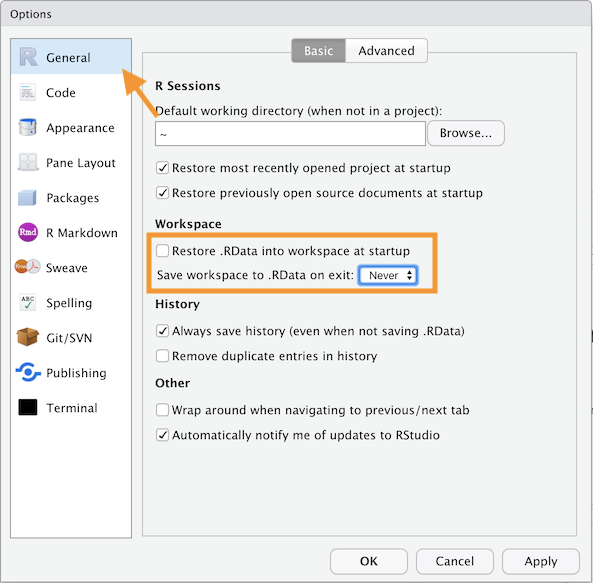
\includegraphics{images/rstudio-startup-and-exit}
    \caption{Réglage de RStudio pour ne pas sauvegarder l'espace
      de travail de R au moment de quitter l'application}
    \label{fig:rstudio:rstudio-startup-and-exit}
  \end{figure}
\item Dans la catégorie \code{Code} et la sous-catégorie
  \code{Editing}, régler l'option \code{Tab width} à \code{4}, tel
  qu'illustré à la \autoref{fig:pratiques:rstudio-tab-width}. Avec ce
  réglage, RStudio indentera par défaut le code de quatre caractères.
  \begin{figure}
    \centering
    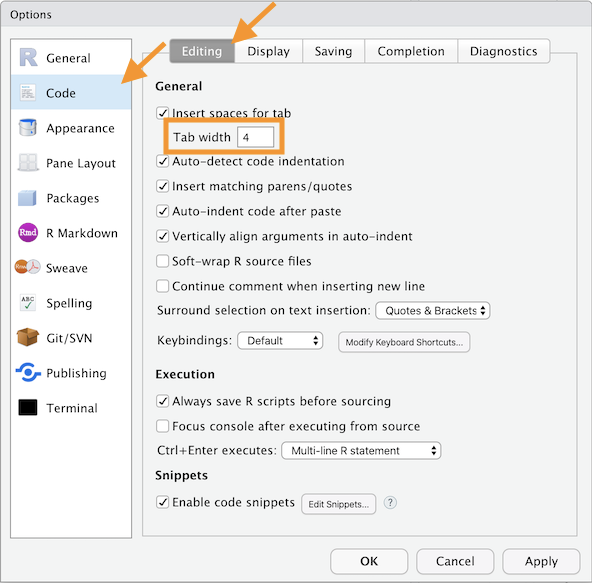
\includegraphics{images/rstudio-tab-width}
    \caption{Réglage de RStudio pour une indentation du code
      de quatre caractères}
    \label{fig:pratiques:rstudio-tab-width}
  \end{figure}
\item Toujours dans la catégorie \code{Code}, mais dans la
  sous-catégorie \code{Saving}, cocher les options \code{Ensure that
    source files end with newline} et \code{Strip trailing horizontal
    whitespace when saving}, puis régler l'option \code{Default text
    encoding} à \code{UTF-8}, tel qu'illustré à la
  \autoref{fig:rstudio:rstudio-utf-8}. RStudio sauvegardera ensuite
  les fichiers de script dans un format portable sur toutes les
  plateformes informatiques et supprimera automatiquement les espaces
  inutiles en fin de ligne.
  \begin{figure}
    \centering
    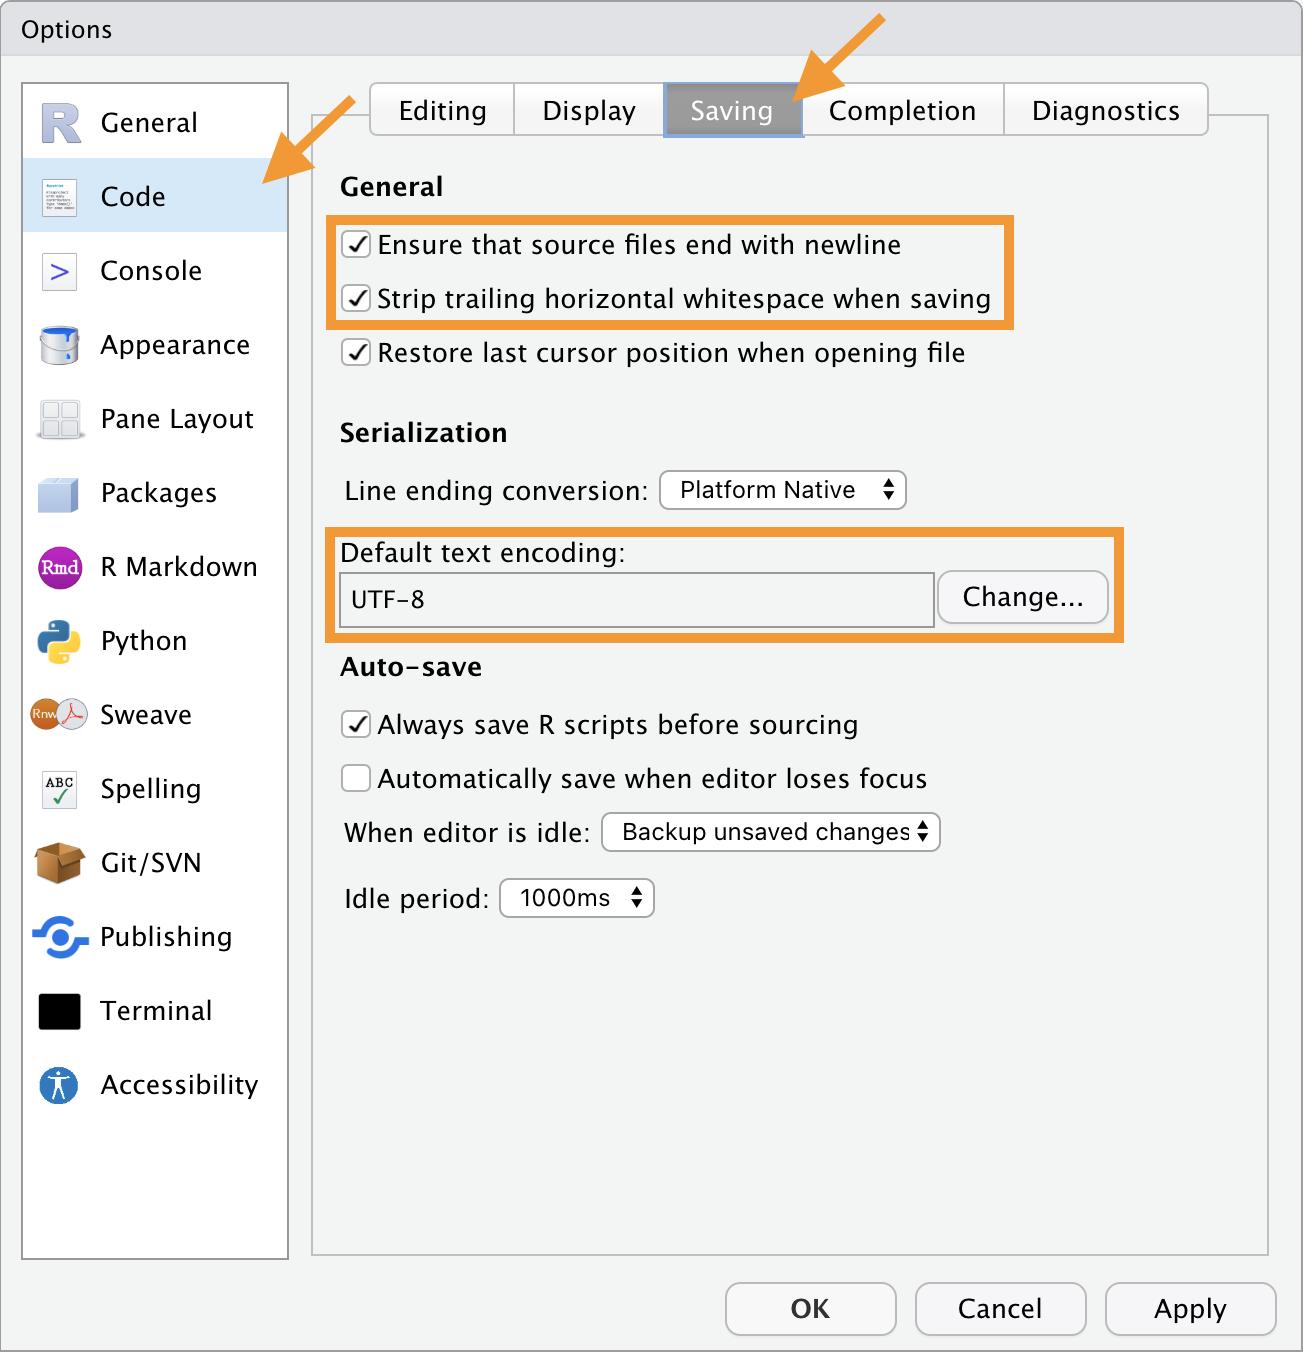
\includegraphics{images/rstudio-utf-8+whitespace}
    \caption{Réglage de RStudio pour la sauvegarde des fichiers dans un
      format portable et sans espaces en fin de ligne}
    \label{fig:rstudio:rstudio-utf-8}
  \end{figure}
\item (Windows seulement) Dans la catégorie \code{Terminal},
  sélectionner \index{Git~Bash}\code{Git~Bash} dans le menu déroulant
  de l'option \code{New Terminals open with}.
\end{enumerate}



\section{Aide et documentation}
\label{sec:rstudio:aide}

La documentation de RStudio se trouve entièrement en ligne. On y
accède par le menu \code{Help}. L'onglet \code{Help} du navigateur de
fichiers (sous-fenêtre en bas à droite) offre également une interface
unifiée pour accéder à l'aide de R et à celle de RStudio.

\index{RStudio|)}

%%% Local Variables:
%%% mode: latex
%%% TeX-engine: xetex
%%% TeX-master: "programmer-avec-r"
%%% coding: utf-8
%%% End:

%%% Copyright (C) 2019 Vincent Goulet
%%%
%%% Ce fichier fait partie du projet
%%% «Programmer avec R»
%%% https://gitlab.com/vigou3/programmer-avec-r
%%%
%%% Cette création est mise à disposition sous licence
%%% Attribution-Partage dans les mêmes conditions 4.0
%%% International de Creative Commons.
%%% https://creativecommons.org/licenses/by-sa/4.0/

\chapter{GNU Emacs et ESS: la base}
\index{Emacs|(}
\label{chap:emacs+ess}

Emacs est l'Éditeur de texte des éditeurs de texte. À l'origine un
éditeur pour les programmeurs (avec des modes spéciaux pour une
multitude de langages différents), Emacs est devenu au fil du temps un
environnement logiciel en soi dans lequel on peut réaliser une foule
de tâches différentes: rédiger des documents {\LaTeX}, interagir avec R,
SAS ou un logiciel de base de données, consulter son courrier
électronique, gérer son calendrier ou même jouer à Tetris!

Cette annexe passe en revue les quelques commandes essentielles pour
commencer à travailler avec GNU Emacs et le mode ESS. L'ouvrage de
\cite{Cameron:Emacs:2004} constitue une excellente référence pour
l'apprentissage plus poussé de l'éditeur.

\setkeys{Gin}{width=370pt} % 1/2 la largeur de l'image insérée
\begin{figure}[t]
  \centering
  \includegraphics{images/emacs.png} \\
  \footnotesize\sffamily\flushleft\vspace{-\baselineskip}%
  Tiré de \href{https://xkcd.com/378/}{XKCD.com}. La commande \code{M-x
    butterfly} existe vraiment dans Emacs\dots\ en référence à cette
  bande dessinée!
\end{figure}
\setkeys{Gin}{width=0.8\textwidth}

\section{Mise en contexte}
\label{sec:emacs+ess:contexte}

Emacs est le logiciel étendard du projet GNU («\emph{GNU is not
  Unix}»), dont le principal commanditaire est la \emph{Free Software
  Foundation} (FSF) à l'origine de tout le mouvement du logiciel
libre. Richard M.\ Stallman, président de la FSF et grand apôtre du
libre, a écrit la première version de Emacs et il continue à ce jour à
contribuer au projet.

Les origines de Emacs remontent au début des années 1980, une époque
où les interfaces graphiques n'existaient pas, le parc informatique
était beaucoup plus hétérogène qu'aujourd'hui (les claviers n'étaient
pas les mêmes d'une marque d'ordinateur à une autre) et les modes de
communication entre les ordinateurs demeuraient rudimentaires.

L'âge vénérable de Emacs transparait à plusieurs endroits, notamment
dans la terminologie inhabituelle, les raccourcis clavier non
conformes aux standards d'aujourd'hui ou la manipulation des fenêtres
qui ne se fait pas avec une souris.

Emacs s'adapte à différentes tâches par l'entremise de \emph{modes}
qui modifient son comportement ou lui ajoutent des fonctionnalités.

L'un de ces modes est ESS \citep[\emph{Emacs Speaks
  Statistics},][]{ESS}. ESS permet d'interagir avec des logiciels
statistiques (en particulier R, S+ et SAS) directement depuis Emacs.
Quelques-uns des développeurs de ESS sont aussi des développeurs de R,
d'où la grande compatibilité entre les deux logiciels. Lorsque ESS est
installé, le mode est activé automatiquement en ouvrant dans Emacs un
fichier dont le nom se termine par l'extension \code{.R}.


\section{Installation}
\label{sec:emacs+ess:installation}

Le présent auteur prépare des distributions modifiées de GNU~Emacs
pour \link{https://vigou3.github.io/emacs-modified-windows/}{Windows}
et pour \link{https://vigou3.github.io/emacs-modified-macos/}{macOS}
qui intègrent le mode ESS.

Sous Linux, GNU Emacs et le mode ESS font normalement partie de toutes
les distributions.

\section{Description sommaire}
\label{sec:emacs+ess:description}

Au lancement, Emacs affiche un écran d'information contenant des liens
vers différentes ressources. Cet écran disparait dès que l'on appuie
sur une touche. La fenêtre Emacs se divise en quatre zones principales
(voir la \autoref{fig:ess:emacswindow}):
\begin{enumerate}
\item tout au haut de la fenêtre (ou de l'écran sous macOS), on trouve
  l'habituelle barre de menu dont le contenu change selon le mode dans
  lequel se trouve Emacs;
\item l'essentiel de la fenêtre sert à afficher un \emph{buffer}, soit
  le contenu d'un fichier ouvert ou l'invite de commande d'un
  programme externe;
\item la ligne de mode est le séparateur horizontal contenant diverses
  informations sur le fichier ouvert et l'état de Emacs;
\item le \emph{minibuffer} est la région au bas de la fenêtre où l'on
  entre des commandes et reçoit de l'information de Emacs.
\end{enumerate}
Il est possible de séparer la fenêtre Emacs en sous-fenêtres pour
afficher plusieurs \emph{buffers} à la fois. Il y a alors une ligne de
mode pour chaque \emph{buffer}.

\begin{figure}[t]
  %% Capture d'écran
  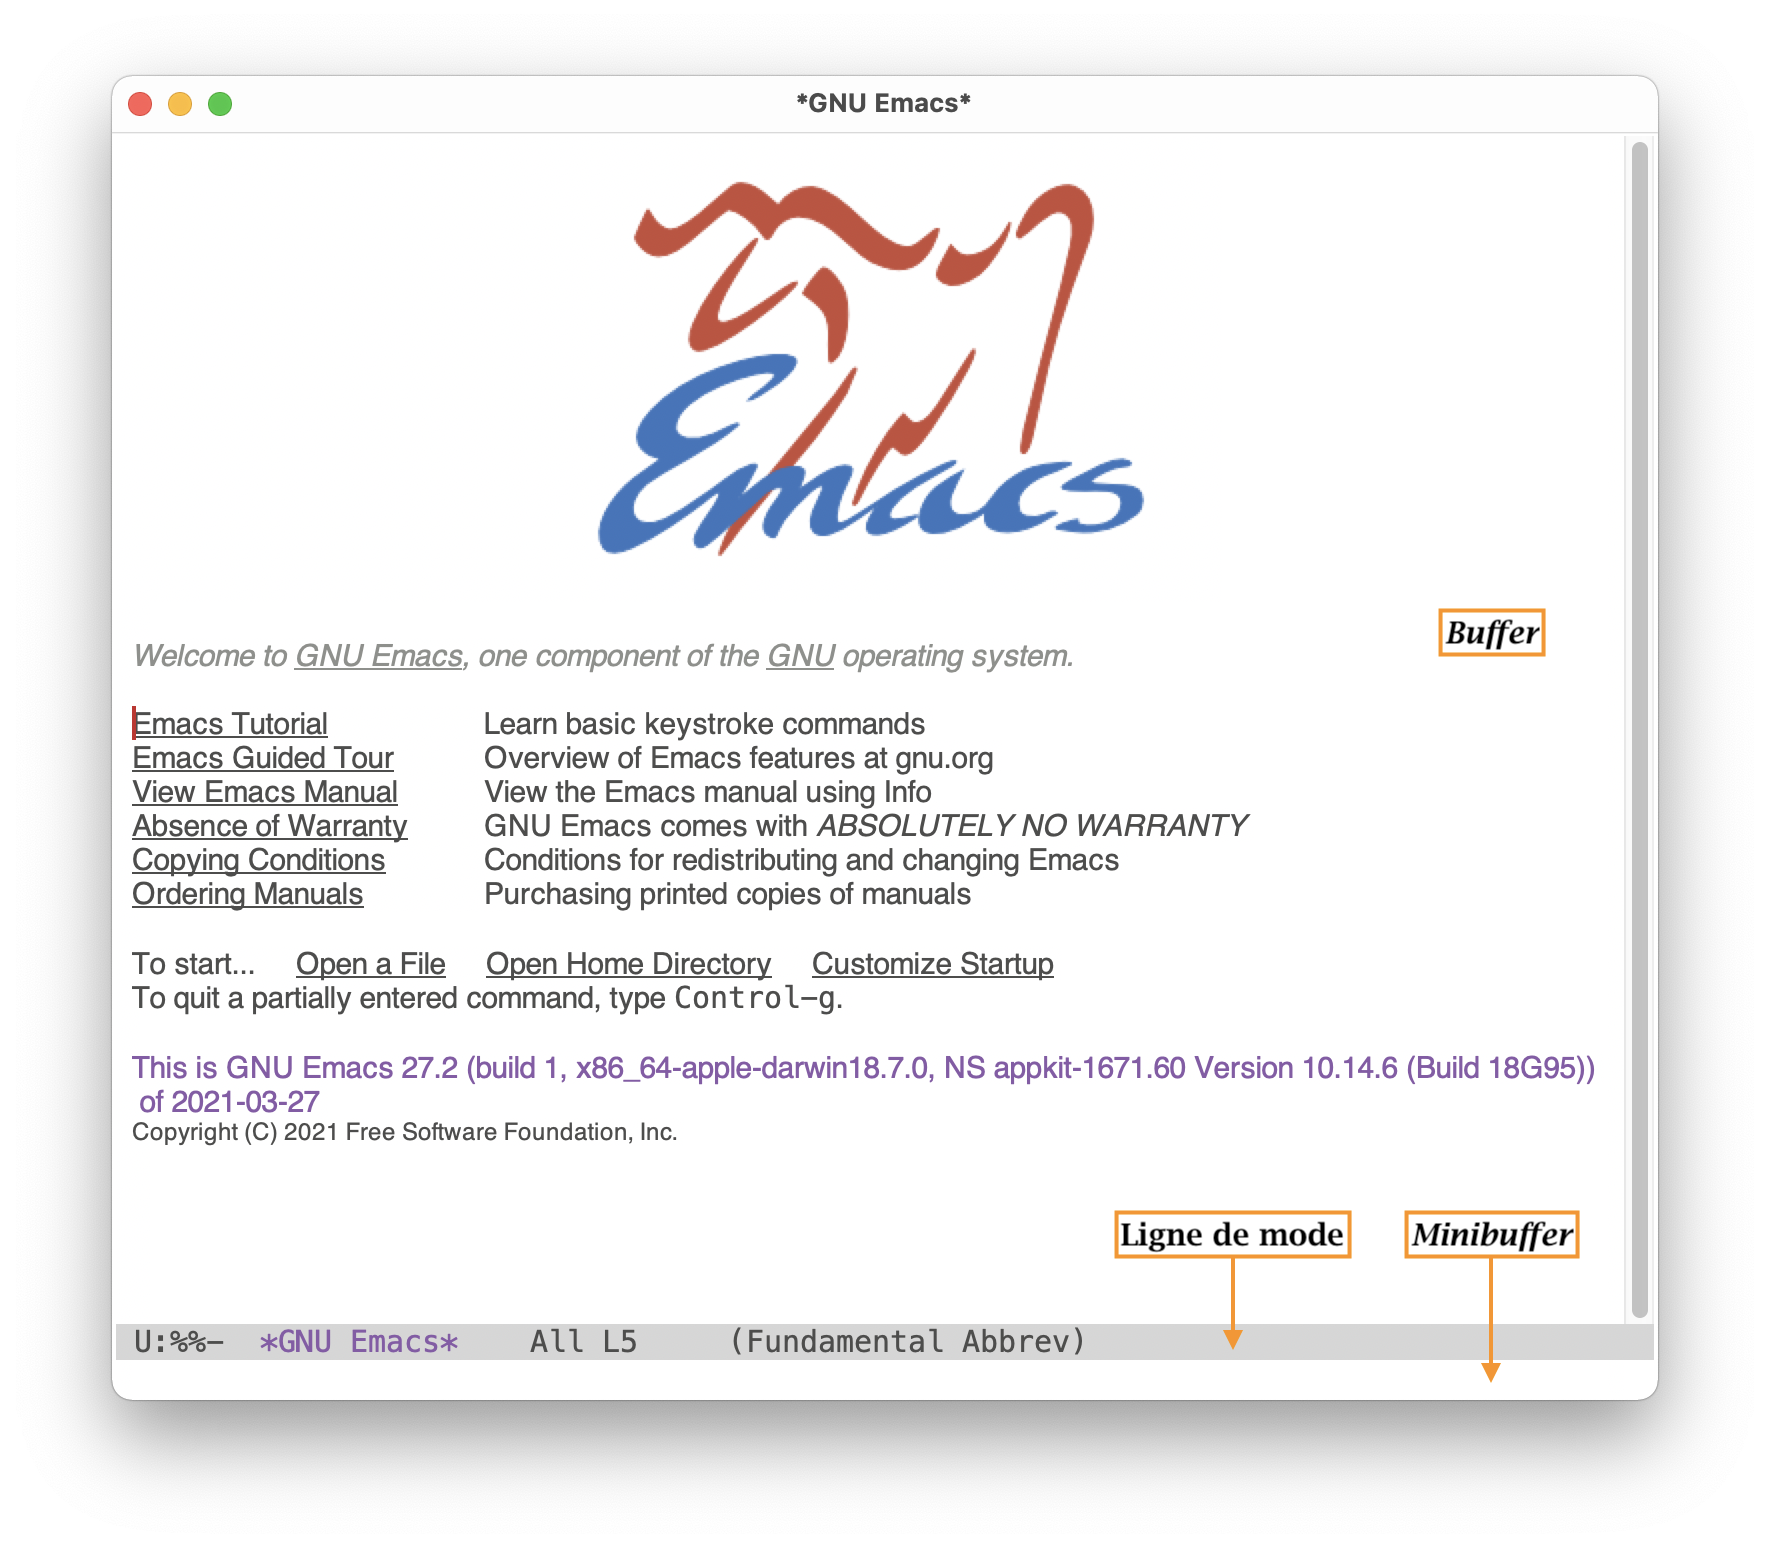
\includegraphics{images/emacswindow-screenshot}

  \begingroup
  \TPoptions{absolute=false}
  %% Identification de la barre de menu
  \begin{textblock}{0.35}(7.38,-6.58)
    \Large\faLongArrowRight
  \end{textblock}
  \begin{textblock}{1.75}(7.88,-6.59)
    \footnotesize\sffamily Barre de menu
  \end{textblock}

  %% Identification du buffer
  \begin{textblock}{0.35}(7.38,-3.38)
    \Large\faLongArrowRight
  \end{textblock}
  \begin{textblock}{1.75}(7.88,-3.39)
    \footnotesize\sffamily \emph{Buffer}
  \end{textblock}

  %% Identification de la mode line
  \begin{textblock}{0.35}(7.38,-0.28)
    \Large\faLongArrowRight
  \end{textblock}
  \begin{textblock}{1.75}(7.88,-0.29)
    \footnotesize\sffamily Ligne de mode
  \end{textblock}

  %% Identification du minibuffer
  \begin{textblock}{0.35}(7.38,-0.08)
    \Large\faLongArrowRight
  \end{textblock}
  \begin{textblock}{1.75}(7.88,-0.09)
    \footnotesize\sffamily \emph{Minibuffer}
  \end{textblock}
  \endgroup
  \caption[Fenêtre de GNU~Emacs sous macOS]{Fenêtre de GNU~Emacs et
    ses différentes parties au lancement de l'application sous macOS.
    Sous Windows et Linux, la barre de menu se trouve à l'intérieur de
    la fenêtre.}
  \label{fig:ess:emacswindow}
\end{figure}


\section{\emph{Emacs-ismes} et \emph{Unix-ismes}}
\label{sec:emacs+ess:ismes}

Emacs possède sa propre terminologie qu'il vaut mieux connaitre
lorsque l'on consulte la documentation. De plus, l'éditeur utilise des
conventions du monde Unix qui sont moins usitées sur les plateformes
Windows et macOS.

\begin{itemize}
\item Dans les définitions de raccourcis claviers:
  \begin{itemize}
  \item \code{C} est la touche \code{Contrôle} (\ctlkey);
  \item \code{M} est la touche \code{Meta}, qui correspond à la touche
    \code{Alt} de gauche sur un PC ou la touche \code{Option}
    (\optkey) sur un Mac (toutefois, voir l'encadré à la
    \autopageref{fig:ess:meta});
  \item \code{ESC} est la touche \code{Échap} (\esckey) et
    est équivalente à \code{Meta};
  \item \code{SPC} est la barre d'espacement;
  \item \code{DEL} est la touche \code{Retour arrière} (\delkey) ---
    \emph{et non la touche} \code{Supprimer}.
  \item \code{RET} est la touche \code{Entrée} (\returnkey);
  \end{itemize}
\item Toutes les fonctionnalités de Emacs correspondent à une commande
  qui peut être tapée dans le \emph{minibuffer}. \code{M-x} démarre
  l'invite de commande.
\item Le caractère \,\verb=~=\, représente le dossier vers lequel
  pointe la variable d'environnement \code{\$HOME} (Linux, macOS) ou
  \code{\%HOME\%} (Windows). C'est le dossier par défaut de Emacs.
\item La barre oblique (\code{/}) est utilisée pour séparer les
  dossiers dans les chemins d'accès aux fichiers, même sous Windows.
\item En général, il est possible d'appuyer sur \code{TAB} dans le
  \emph{minibuffer} pour compléter les noms de fichiers ou de
  commandes.
\end{itemize}

\begin{figure}[t]
  \refstepcounter{dummy}
  \label{fig:ess:meta}
  \begin{titled-frame}{Configuration de la touche Meta sous macOS}
    Par défaut sous macOS, la touche \code{Meta} est assignée à
    \code{Option} (\optkey). Sur les claviers français, cela empêche
    d'accéder à certains caractères spéciaux tels que {\og}[{\fg},
    «]», «\{» ou «\}».

    Une solution à cette fâcheuse situation consiste à assigner
    la touche \code{Meta} à \code{Commande} (\cmdkey). Cela bloque
    alors l'accès à certains raccourcis Mac, mais la situation est
    moins critique ainsi.

    Pour assigner la touche \code{Meta} à \code{Commande} (\cmdkey) et
    laisser la touche \code{Option} (\optkey) jouer son rôle usuel, il
    suffit d'insérer les lignes suivantes dans son fichier de
    configuration \code{.emacs} (voir la
    \autoref{sec:emacs+ess:configuration}):
\begin{verbatim}
(setq-default ns-command-modifier 'meta)
(setq-default ns-option-modifier 'none)
\end{verbatim}
  \end{titled-frame}
\end{figure}



\section{Commandes de base}
\label{sec:emacs+ess:commandes}

Emacs comporte une pléthore de commandes, il serait donc futile de
tenter d'en faire une liste exhaustive ici. Nous nous contenterons de
mentionner les commandes les plus importantes regroupées par tâche.

\subsection{Les essentielles}
\label{sec:emacs+ess:commandes:essentielles}

\begin{ttscript}{M-x}
\item[\code{M-x}] démarrer l'invite de commande
\item[\code{C-g}] bouton de panique: annuler, quitter! Presser plus
  d'une fois au besoin.
\end{ttscript}

\subsection{Manipulation de fichiers}
\label{sec:emacs+ess:commandes:fichiers}

Entre parenthèses, le nom de la commande Emacs correspondante. On peut
entrer cette commande dans le \emph{minibuffer} au lieu d'utiliser le
raccourci clavier.

\tipbox{Il n'existe pas de commande «nouveau
  fichier» dans Emacs. Pour créer un nouveau fichier, il suffit
  d'ouvrir un fichier qui n'existe pas déjà.\index{Emacs!nouveau fichier}}

\begin{ttscript}{C-x C-w}
\item[\code{C-x C-f}] ouvrir un fichier (\code{find-file})
\item[\code{C-x C-s}] sauvegarder
  (\code{save-buffer})\index{Emacs!sauvegarder}
\item[\code{C-x C-w}] sauvegarder sous
  (\code{write-file})\index{Emacs!sauvegarder sous}
\item[\code{C-x k}] fermer un fichier (\code{kill-buffer})
  \\[\baselineskip]
\item[\code{C-\_}] annuler (pratiquement illimité); aussi
  \code{C-x u} (\code{undo})
  \\
\item[\code{C-s}] recherche incrémentale avant
  (\code{isearch-forward})
\item[\code{C-r}] Recherche incrémentale arrière
  (\code{isearch-backward})
\item[\code{M-\%}] rechercher et remplacer
  (\code{query-replace})\index{Emacs!rechercher et remplacer}
\end{ttscript}


\subsection{Déplacements simples du curseur}
\index{Emacs!déplacement du curseur}
\label{sec:emacs+ess:commandes:deplacement}

\begin{ttscript}{C-DEL | C-w}
\item[\code{C-b} | \code{C-f}] déplacer d'un caractère vers
  l'arrière~|~l'avant \newline
  (\code{backward-char} | \code{forward-char})
\item[\code{C-a} | \code{C-e}] aller au début~|~fin de la ligne \newline
  (\code{move-beginning-of-line} | \code{move-end-of-line})
\item[\code{C-p} | \code{C-n}] aller à la ligne précédente~|~suivante \newline
  (\code{previous-line} | \code{next-line})
\item[\code{M-<} | \code{M->}] aller au début~|~fin du fichier \newline
  (\code{beginning-of-buffer} | \code{end-of-buffer})
  \\
\item[\code{DEL} | \code{C-d}] effacer le caractère à
  gauche~|~droite du curseur  \newline
  (\code{delete-backward-char} | \code{delete-char})
\item[\code{M-DEL} | \code{M-d}] effacer le mot à gauche~|~droite
  du curseur  \newline
  (\code{backward-kill-word} | \code{kill-word})
\item[\code{C-k}] supprimer jusqu'à la fin de la ligne (\code{kill-line})
\end{ttscript}

\osxbox{Plusieurs des raccourcis clavier de Emacs composés avec la
  touche \code{Contrôle} (\ctlkey) sont valides sous macOS. Par
  exemple, \ctlkey\,\code{A} et \ctlkey\,\code{E} déplacent le curseur
  au début et à la fin de la ligne dans les champs texte.}


\subsection{Sélection de texte, copier, coller, couper}
\index{Emacs!sélection}
\label{sec:emacs+ess:commandes:selection}

\begin{ttscript}{C-x C-w}
\item[\code{C-SPC}] débute la sélection (\code{set-mark-command})
\item[\code{C-w}] couper la sélection (\code{kill-region})
\item[\code{M-w}] copier la sélection (\code{kill-ring-save})
\item[\code{C-y}] coller (\code{yank})
\item[\code{M-y}] remplacer le dernier texte collé par la
  sélection précédente \newline
  (\code{yank-pop})
\end{ttscript}

\tipbox{Il est possible d'utiliser les raccourcis clavier usuels de
  Windows (\code{C-c}, \code{C-x}, \code{C-v}) et macOS
  (\cmdkey\,\code{C}, \cmdkey\,\code{X}, \cmdkey\,\code{V}) en
  activant le mode CUA dans le menu \code{Options}.}

\windowsbox{ On peut copier-coller directement avec la souris dans Windows en
  sélectionnant du texte puis en appuyant sur le bouton central (ou la
  molette) à l'endroit souhaité pour y copier le texte.}


\subsection{Manipulation de fenêtres}
\label{sec:emacs+ess:commandes:fenetres}

\begin{ttscript}{C-x C-w}
\item[\code{C-x b}] changer de \emph{buffer}
  (\code{switch-buffer})
\item[\code{C-x 2}] séparer l'écran en deux fenêtres
  (\code{split-window-vertically})
\item[\code{C-x 1}] conserver uniquement la fenêtre courante \newline
  (\code{delete-other-windows})
\item[\code{C-x 0}] fermer la fenêtre courante
  (\code{delete-window})
\item[\code{C-x o}] aller vers une autre fenêtre lorsqu'il y en a
  plus d'une \newline
  (\code{other-window})
\end{ttscript}

\subsection{Manipulation de fichiers de script dans le mode ESS}
\index{Emacs!mode ESS|(}
\label{sec:emacs+ess:commandes:script}

Le mode ESS dispose de fonctions «intelligentes» qui facilitent
grandement la manipulation des fichiers de script. Les deux
principales commandes à connaitre sont les suivantes:
\begin{ttscript}{C-x C-w}
\item[\code{C-RET}] évaluer dans le processus R la ligne sous le
  curseur ou la région sélectionnée, puis déplacer le curseur à la
  prochaine expression \newline
  (\code{ess-eval-region-or-line-and-step})
\item[\code{C-c C-c}] évaluer dans le processus R la région
  sélectionnée, la fonction ou le paragraphe (tout bloc entre deux
  lignes blanches) dans lequel se trouve le curseur, puis déplacer le
  curseur à la prochaine expression \newline
  (\code{ess-eval-region-or-function-or-paragraph-and-step})
\end{ttscript}
Les quelques autres fonctions utiles sont:
\begin{ttscript}{C-x C-w}
\item[\code{\_}] insérer le symbole d'affectation \verb*| <- | (sauf
  dans les champs texte et dans les commentaires);
  appuyer deux fois consécutives pour obtenir le caractère de
  soulignement \newline
  (\code{ess-smart-S-assign})
\item[\code{C-c C-z}] déplacer le curseur vers le processus R \newline
  (\code{ess-switch-to-inferior-or-script-buffer})
\item[\code{C-c C-f}] évaluer le code de la fonction courante dans
  le processus R \newline
  (\code{ess-eval-function})
\item[\code{C-c C-l}] évaluer le code du fichier courant en entier dans
  le processus R \newline
  (\code{ess-load-file})
\item[\code{C-c C-v}] aide sur une commande R
  (\code{ess-display-help-on-object})
\end{ttscript}

\subsection{Interaction avec l'invite de commande R}
\label{sec:emacs+ess:commandes:invite}

\begin{ttscript}{M-p |M-n}
\item[\code{M-p} | \code{M-n}] commande précédente~|~suivante
  dans l'historique \newline
  (\code{previous-matching-history-from-input} | \newline
  \code{next-matching-history-from-input})
\item[\code{C-c C-z}] déplacer le curseur vers le fichier de script
  courant \newline
  (\code{ess-switch-to-inferior-or-script-buffer})
\item[\code{M-h}] sélectionner le résultat de la dernière commande \newline
  (\code{mark-paragraph})
\item[\code{C-c C-o}] effacer le résultat de la dernière commande \newline
  (\code{comint-delete-output})
\item[\code{C-c C-v}] aide sur une commande R
  (\code{ess-display-help-on-object})
\item[\code{C-c C-q}] terminer le processus R (\code{ess-quit})
\end{ttscript}

\subsection{Consultation des rubriques d'aide de R}
\label{sec:emacs+ess:commandes:aide}

\begin{ttscript}{m, m}
\item[\code{p} | \code{n}] aller à la section précédente~|~suivante de
  la rubrique \newline
  (\code{ess-skip-to-previous-section} |
  \code{ess-skip-to-next-section})
\item[\code{s a}] aller à la section de la liste des arguments \emph{(Arguments)}
\item[\code{s D}] aller à la section des détails sur la fonction \emph{(Details)}
\item[\code{s v}] aller à la section sur la valeur retournée par la
  fonction \emph{(Value)}
\item[\code{s s}] aller à la section des fonctions apparentée \emph{(See Also)}
\item[\code{s e}] aller à la section des exemples \emph{(Examples)}
\item[\code{l}] évaluer la ligne sous le curseur; pratique pour
  exécuter les exemples \newline
  (\code{ess-eval-line-and-step})
\item[\code{r}] évaluer la région sélectionnée (\code{ess-eval-region})
\item[\code{h}] ouvrir une nouvelle rubrique d'aide, par défaut pour
  le mot se trouvant sous le curseur
  (\code{ess-display-help-on-object})
\item[\code{q}] retourner au processus ESS en laissant la rubrique
  d'aide visible \newline
  (\code{ess-switch-to-end-of-ESS})
\item[\code{x}] fermer la rubrique d'aide et retourner au processus
  ESS \newline
  (\code{ess-kill-buffer-and-go})
\end{ttscript}



\section{Anatomie d'une session de travail (ter)}
\label{sec:emacs+ess:session}

On reprend ici la description de la type présentée à la
\autoref{sec:presentation:session}, mais en expliquant comment
compléter chaque étape dans Emacs avec le mode ESS. Sont intercalés
dans les instructions les raccourcis clavier des commandes Emacs et
les accès par les menus, le cas échéant.

\begin{enumerate}
\item Lancer Emacs et ouvrir un fichier de script.
  \begin{trivlist}
  \item
    \makebox[0.28\linewidth][l]{%
      \colorbox{codebg}{\code{C-x C-f}}}
    \hfill
    \makebox[0.68\linewidth][l]{%
      \colorbox{codebg}{\code{File|Open File...}}}
  \end{trivlist}
  En spécifiant un nom de fichier qui n'existe pas déjà, on crée un
  nouveau fichier de script. S'assurer de terminer le nom du nouveau
  fichier par \code{.R} pour que Emacs reconnaisse automatiquement
  qu'il s'agit d'un fichier de script R.
\item Démarrer un processus R à l'intérieur de Emacs.
  \begin{trivlist}
  \item
    \makebox[0.28\linewidth][l]{%
      \colorbox{codebg}{\code{M-x R }\returnkey}}
  \end{trivlist}
  Emacs demandera de spécifier de répertoire de travail
  (\emph{starting data directory}). Accepter la valeur par défaut ou
  indiquer un autre dossier.
  \begin{trivlist}
  \item
    \makebox[0.28\linewidth][l]{%
      \colorbox{codebg}{\code{\textasciitilde/ = }\returnkey}}
  \end{trivlist}
  Un éventuel message de Emacs à l'effet que le fichier
  \code{.Rhistory} n'a pas été trouvé est sans conséquence et peut
  être ignoré.
\item Composer le code. Lors de cette étape, on se déplacera souvent
  du fichier de script à la ligne de commande afin d'essayer diverses
  expressions. On exécutera également des parties seulement du code se
  trouvant dans le fichier de script. Les commandes les plus utilisées
  sont alors:
  \begin{trivlist}
  \item
    \makebox[0.28\linewidth][l]{%
      \colorbox{codebg}{\code{C+RET}}}
    \hfill
    \makebox[0.68\linewidth][l]{%
      \colorbox{codebg}{\code{ESS|Eval region | line}}}
  \item
    \makebox[0.28\linewidth][l]{%
      \colorbox{codebg}{\code{C-c C-c}}}
    \hfill
    \makebox[0.68\linewidth][l]{%
      \colorbox{codebg}{\code{ESS|Eval region | func | para \& step}}}
  \item
    \makebox[0.28\linewidth][l]{%
      \colorbox{codebg}{\code{C-c C-z}}}
    \hfill
    \makebox[0.68\linewidth][l]{%
      \colorbox{codebg}{\code{ESS|Process|Switch to process buffer}}}
  \end{trivlist}
\item Sauvegarder le fichier de script.
  \begin{trivlist}
  \item
    \makebox[0.28\linewidth][l]{%
      \colorbox{codebg}{\code{C-x C-s}}}
    \hfill
    \makebox[0.68\linewidth][l]{%
      \colorbox{codebg}{\code{File|Save}}}
  \end{trivlist}
  Les quatrième et cinquième caractères de la ligne de mode changent
  de \,\verb|**|\, à \,\verb|--|.
\item Sauvegarder si désiré l'espace de travail de R avec
  \code{save.image()}\index{save.image@\code{save.image}}. Cela n'est
  habituellement pas nécessaire à moins que l'espace de travail ne
  contienne des objets importants ou longs à recréer.
\item Quitter le processus R.
  \begin{trivlist}
  \item
    \makebox[0.28\linewidth][l]{%
      \colorbox{codebg}{\code{C-c C-q}}}
    \hfill
    \makebox[0.68\linewidth][l]{%
      \colorbox{codebg}{\code{iESS|Quit}}}
  \end{trivlist}
  Cette commande de ESS se charge de fermer tous les fichiers associés
  au processus R. On peut ensuite quitter Emacs en fermant
  l'application de la manière usuelle.
\end{enumerate}
\index{Emacs!mode ESS|)}

\videobox{\link{https://youtu.be/KtmFDm2AKM4}{Anatomie d'une session de travail
    avec GNU Emacs}}{%
  La session de travail type avec GNU Emacs ci-dessus fait aussi l'objet
  d'\link{https://youtu.be/KtmFDm2AKM4}{une vidéo}.}


\section{Configuration de l'éditeur}
\label{sec:emacs+ess:configuration}

Une des grandes forces de Emacs est qu'à peu près chacune de ses
facettes est configurable: couleurs, polices de caractère, raccourcis
clavier, etc.

La configuration de Emacs repose sur des commandes réunies dans un
nommé \code{.emacs} (le point est important!) que Emacs lit au
démarrage. Le fichier \code{.emacs} doit se trouver dans le dossier
\,\verb=~/=, c'est-à-dire dans le dossier de départ de l'utilisateur
sous Linux et macOS, et dans le dossier référencé par la variable
d'environnement \code{\%HOME\%} sous Windows.

\videobox{\link{https://youtu.be/jdtjBBkfhO0}{Création de fichiers de
    configuration pour Emacs et R}}{%
  Visionnez la vidéo portant sur la
  \link{https://youtu.be/jdtjBBkfhO0}{création de fichiers de
    configuration} pour Emacs et R.}


\section{Aide et documentation}
\label{sec:emacs+ess:aide}

Emacs possède son propre système d'aide très exhaustif, mais dont la
navigation est peu intuitive selon les standards d'aujourd'hui.
Consulter le menu \code{Help}.

Autrement, on trouvera dans les sites respectifs des deux projets les
manuels de \link{https://www.gnu.org/software/emacs}{Emacs} et de
\link{https://ess.r-project.org}{ESS}.

Enfin, si le désespoir vous prend au cours d'une séance de codage
intensive, vous pouvez toujours consulter le psychothérapeute Emacs.
On le trouve, bien entendu, dans le menu \code{Help}!

\index{Emacs|)}

%%% Local Variables:
%%% mode: latex
%%% TeX-engine: xetex
%%% TeX-master: "programmer-avec-r"
%%% coding: utf-8
%%% End:

%%% Copyright (C) 2017-2022 Vincent Goulet
%%%
%%% Ce fichier fait partie du projet
%%% «Programmer avec R»
%%% https://gitlab.com/vigou3/programmer-avec-r
%%%
%%% Cette création est mise à disposition sous licence
%%% Attribution-Partage dans les mêmes conditions 4.0
%%% International de Creative Commons.
%%% https://creativecommons.org/licenses/by-sa/4.0/

\chapter{Solutions des exercices}
\label{chap:solutions}

%% Ce fichier ne sert qu'à disposer les solutions des exercices à la
%% fin du document. Le texte des solutions se trouve avec leur
%% exercice correspondant, dans les fichiers des chapitres.

\input{solutions-informatique}
\input{solutions-algorithmes}
\input{solutions-bases}
\input{solutions-donnees}
\input{solutions-pratiques}
\input{solutions-tri}
\input{solutions-debogage}
\input{solutions-import-export}
\input{solutions-texte}
\input{solutions-environnement}

%%% Local Variables:
%%% mode: latex
%%% TeX-engine: xetex
%%% TeX-master: "programmer-avec-r"
%%% coding: utf-8
%%% End:


\bibliography{r,stat,informatique,vg}

\cleardoublepage
\printindex

\pagestyle{empty}

\cleartoverso
%%% Copyright (C) 2014-2024 Vincent Goulet
%%%
%%% Ce fichier fait partie du projet
%%% «Programmer avec R»
%%% https://gitlab.com/vigou3/programmer-avec-r
%%%
%%% Cette création est mise à disposition sous licence
%%% Attribution-Partage dans les mêmes conditions 4.0
%%% International de Creative Commons.
%%% https://creativecommons.org/licenses/by-sa/4.0/

\vspace*{\fill}

\begingroup
\calccentering{\unitlength}
\begin{adjustwidth*}{\unitlength}{-\unitlength}
  \begin{flushleft}
    \small %
    Ce document a été produit avec le système de mise en page
    {\XeLaTeX}. Le texte principal est composé en Lucida Bright~OT
    11~points, les mathématiques en Lucida Bright Math~OT, le code
    informatique en Lucida Grande Mono~DK et les titres en Fira~Sans.
    Des icônes proviennent de la police Font~Awesome. Les graphiques
    ont été réalisés avec R.
  \end{flushleft}
\end{adjustwidth*}
\endgroup
\vfill


\cleartoverso
%%% Copyright (C) 2021 Vincent Goulet
%%%
%%% Ce fichier fait partie du projet
%%% «Programmer avec R»
%%% https://gitlab.com/vigou3/programmer-avec-r
%%%
%%% Cette création est mise à disposition sous licence
%%% Attribution-Partage dans les mêmes conditions 4.0
%%% International de Creative Commons.
%%% https://creativecommons.org/licenses/by-sa/4.0/

\begingroup
\TPGrid{8}{64}
\textblockorigin{0mm}{0mm}
\setlength{\parindent}{0mm}
\setlength{\bandeorwidth}{12.8125\TPVertModule} % == 4\logoheight
\setlength{\banderougewidth}{\paperwidth}
\addtolength{\banderougewidth}{-\bandeorwidth}
\setlength{\bandeorheight}{\TPVertModule}
\setlength{\banderougeheight}{\TPVertModule}

%% bandeau identitaire arrière
\begin{textblock*}{\paperwidth}[0,1](0mm,56\TPVertModule)
  \textcolor{or}{\rule{\bandeorwidth}{\TPVertModule}}%      % bande or
  \textcolor{rouge}{\rule{\banderougewidth}{\TPVertModule}} % bande rouge
\end{textblock*}
\endgroup

%%% Local Variables:
%%% mode: latex
%%% TeX-master: "programmer-avec-r"
%%% TeX-engine: xetex
%%% End:


\end{document}

%%% Local Variables:
%%% mode: latex
%%% TeX-engine: xetex
%%% TeX-master: t
%%% coding: utf-8
%%% End:
